\documentclass[a4paper, oneside, 12pt, english, ngerman]{article}
\usepackage{setspace}
\usepackage{graphicx}
\usepackage{geometry}
\usepackage[acronym]{glossaries}
\usepackage[toc,page]{appendix}
\usepackage{titling}
\usepackage[utf8]{inputenc}
\usepackage{url}
\usepackage{color,soul}
\usepackage{csquotes}
\usepackage{float}
\usepackage{listings}
\usepackage{subcaption}
\usepackage{tabularx}
\usepackage{enumitem}
\usepackage{multirow}
\usepackage{tabularx}
\usepackage{booktabs} 
\usepackage{cellspace}
\usepackage{amssymb}
\usepackage{algorithm}
\usepackage{algpseudocode}
\usepackage{rotating}
\usepackage{afterpage}
\usepackage{svg}
\usepackage[export]{adjustbox}
\usepackage{fancyhdr}
\usepackage[labelfont=bf]{caption}
\captionsetup{labelsep=space}
\usepackage{threeparttable}
\usepackage{pdfpages}
\usepackage[style=ieee,backend=biber,language=english]{biblatex}
\usepackage[hidelinks]{hyperref}
\usepackage{tikz}
\usetikzlibrary{matrix, positioning, shapes.geometric, arrows.meta}

\setlength{\headheight}{30pt}
\fancypagestyle{main}{
  \fancyhf{}
  \fancyhead[R]{\MakeUppercase{\leftmark}}
  \fancyfoot[C]{\thepage}
  \renewcommand{\headrulewidth}{0.4pt}
  \pagenumbering{arabic}
}

\fancypagestyle{plain}{
  \fancyhf{}
  \fancyfoot[C]{\thepage}
  \renewcommand{\headrulewidth}{0pt}
  \pagenumbering{Roman}
}

\fancypagestyle{blank}{
  \fancyhf{}
  \pagenumbering{arabic}
  \renewcommand{\headrulewidth}{0pt}
}

\addbibresource{lists/biliography.bib}

\graphicspath{ {./figures/title/}, {./figures/02_background/}, {./figures/04_results/}, {./figures/appendix/} }

\setlength{\cellspacetoplimit}{8pt}
\setlength{\cellspacebottomlimit}{8pt}

\newcommand{\art}{Masterarbeit}
\newcommand{\fachgebiet}{Medieninformatik}
\newcommand{\titelname}{Selective Genetic Distance Computation for Visualizing Viral Outbreak Dynamics}
\newcommand{\authorname}{Ben Kräling}
\newcommand{\matnr}{902480}
\newcommand{\supervisor}{Prof.\,Dr.\,Florian Huber}
\newcommand{\secsupervisor}{Univ-Prof.\,Dr.\,Alexander Dilthey}
\newcommand{\jahr}{2025}
\newcommand{\ACRFULL}[1]{\MakeUppercase{\acrfull{#1}}}

\geometry{margin=2.54cm, left=3.8cm}

\makeglossaries
\loadglsentries{./lists/glossary}
    
\begin{document}
    \frenchspacing
    \setstretch{1.5}
    \begin{titlepage}
    
\includegraphics[height=1cm, right] {hds_medien_logo_bunt}\\[15ex]
    \begin{center}
    
    \LARGE{\textbf{\art}}\\[1ex]
    \Large{im Fachgebiet \fachgebiet}\\[6ex]
    \Large{\textbf{\titelname}}\\[6ex]
    
    \normalsize
    \begin{tabular}{p{3cm}p{6.4cm}}\\
        vorgelegt von:  & \quad \authorname \\[1.2ex]
        Studienbereich: & \quad \fachgebiet \\[1.2ex]
        Matrikelnummer: & \quad \matnr \\[1.2ex]
        Erstgutachter:  & \quad \supervisor\\[1.2ex]
        Zweitgutachter: & \quad \secsupervisor\\
    \end{tabular}
    \end{center}
\setcounter{page}{1}
\end{titlepage}
    \pagestyle{blank}
    \vspace*{\fill}
\singlespacing
{\small \noindent Dieses Werk ist urheberrechtlich geschützt.\\ 
Jede Nutzung außerhalb der engen Grenzen des Urheberrechtsgesetzes ist ohne Zustimmung des Autors unzulässig. Dies gilt insbesondere für Vervielfältigungen, Übersetzungen, Mikroverfilmungen sowie die Speicherung und Verarbeitung in elektronischen Systemen.\\[0.5em]}

\noindent \copyright~\authorname, \jahr \\
\frenchspacing
\setstretch{1.5}


    \clearpage
    \section*{Eidesstattliche Erklärung}
\begin{spacing}{1.5}
Hiermit versichere ich, dass ich meine Masterarbeit mit dem Titel "\titelname" eigenständig und ohne unzulässige fremde Hilfe verfasst habe. Ich habe keine anderen als die angegebenen Quellen und Hilfsmittel benutzt und die aus fremden Quellen direkt oder indirekt übernommenen Inhalte als solche kenntlich gemacht. Diese Aussage trifft auch für alle Implementierungen und Dokumentationen im Rahmen dieses Projektes zu. Die Arbeit hat in gleicher oder ähnlicher Form noch in keinem Prüfungsverfahren vorgelegen. Sie wurde bisher auch nicht veröffentlicht.
\vspace{3cm}

\noindent\textbf{\authorname}

\noindent Düsseldorf, den 08. August 2025
\end{spacing}

    \clearpage
    \section*{Acknowledgments}
\noindent First, I express my gratitude to my first supervisor, Prof. Dr. Florian Huber, for the regular feedback meetings and constructive comments he provided throughout the development of this thesis. I also thank my second supervisor, Univ.-Prof. Dr. Alexander Dilthey, for his feedback, helpful discussions, and insights into bioinformatics. I am also grateful to both of them for giving me the opportunity of being part of the GENTRAIN team.
\par\vspace{1em} 
\noindent Special thanks to my fellow students, colleagues, friends, and family who supported me during this journey, both academically and personally. My deepest gratitude goes to my close friend, Matthias Faska, and my partner, Isabell Mayer, for their unwavering encouragement and uplifting words.

    \clearpage
    \section*{Abstract}
The growing significance of disease outbreak analysis, in conjunction with enhanced genome sequence availability, necessitates the development of user-oriented applications that facilitate genetic outbreak analysis for non-specialists. Since the computational effort involved in visualizing genetic outbreak dynamics increases significantly with the number of sequences considered, this work aims to reduce the effort required to visualize outbreak dynamics while preserving interpretability for outbreak analysis. Key contributions include the algorithmic modification of single genetic distance calculations, as well as the calculation of sparse genetic distance matrices through genetic distance approximation and approximate nearest neighbor search. The proposed approaches exhibit a high degree of accuracy in preserving infection chains and outbreak-related contexts, while significantly reducing the necessary runtime. In general, longer seasonal periods and wider geographic areas tend to yield superior preservation of outbreak characteristics.

\section*{Zusammenfassung}
Die zunehmende Bedeutung der Analyse von Infektionsketten sowie die verbesserte Verfügbarkeit von Genomsequenzen unterstreichen die Notwendigkeit nutzerfreundlicher Anwendungen, die genetisch gestützte Ausbruchsanalysen vereinfachen. Aufgrund der signifikanten Erhöhung des notwendigen rechnerischen Aufwands zur Visualisierung genetischer Ausbruchsszenarien ist das Ziel dieser Arbeit, diesen Aufwand zu reduzieren und gleichzeitig die Interpretierbarkeit für Ausbruchsanalysen bestmöglich beizubehalten. Zu diesem Zweck wurde die Berechnung der genetischen Distanz optimiert und selektive Berechnungen genetischer Distanzmatrizen auf Basis von Distanzapproximationen sowie mittels Approximate Nearest Neighbor Search durchgeführt.
Die vorgestellten Methoden bewahren Infektionsketten und ausbruchsbezogene Kontexte weitgehend, während die notwendige Laufzeit drastisch reduziert wird. Grundsätzlich ist festzuhalten, dass die Betrachtung längerer Zeiträume und größerer geografischer Bereiche die Erhaltung von Ausbruchs-Charakteristika fördert.
    \clearpage
    \pagestyle{plain}
    \tableofcontents
    \cleardoublepage
    \listoffigures
    \cleardoublepage
    \listoftables
    \clearpage
    \singlespacing
    \printglossary[type=\acronymtype]
    \newpage
    \pagestyle{main}
    \frenchspacing
    \setstretch{1.5}
    \setcounter{page}{1}
    \section{Introduction}
\label{cha:introduction}
When the SARS-CoV-2 pandemic emerged in 2019, the world was faced with the immense challenge of understanding and containing a new virus. Local health authorities were overwhelmed by the effort required to identify contacts and outbreak scenarios, a process that relied mainly on interviewing infected individuals.
This global pressure, coupled with the recent expansion of genomic sequencing technologies, has resulted in increased genome sequencing efforts around the world. Observing the genomic structure, and particularly its evolutionary characteristics, provides biological evidence and insight into infection chains. This enables a rapid public health response to changing viral outbreak dynamics, as was demonstrated during the SARS-CoV-2 pandemic. However, genomic data analysis is a complex field that is not yet very user-oriented due to the immense runtime of its underlying algorithms and the high level of expertise required. In scenarios with greater availability of genome sequences, such as in large geographic areas or over longer seasonal periods, the time required for these processes exceeds the timeframe within which public health responses must be decided.

The GENTRAIN project is just one example of a user-oriented application that emerged from the exceptional situation caused by the SARS-CoV-2 pandemic \cite{Fra1}. The project was launched by the state government of North Rhine-Westphalia and funded by the European Union to support local public health authorities in conducting outbreak analyzes that combine contact tracing data with visualizations of the underlying infection chains. These visualizations are based on genetic distance matrices, which are made up of genetic distances between all isolates in a given dataset. While the calculation of these matrices is relatively efficient for confined municipal scenarios, it is not well-suited for large-scale scenarios due to its quadratic scaling with the number of genomes observed. Furthermore, GENTRAIN attaches great importance to the accurate determination of low genetic distances, particularly because its focus is on the identification and tracking of infection chains. This requires a more complex algorithm to calculate a single genetic distance, which results in longer computation times for individual calculations.

The objective of this work is to approach this problem scientifically by providing solutions that allow for the analysis of viral outbreaks in larger but still plausible scenarios.
Given the direct proportionality between the calculation time of genetic distance matrices and the number of sequences considered, the methodological approach of this work is designed to identify and consider only the most relevant distances in a genetic distance matrix. This approach was taken with a focus on preserving the interpretability of the visualization to the greatest extent feasible.
The subsequent research question is therefore posed: 

\vspace{10pt}
\noindent
\textit{"How can the computational effort involved in visualizing large-scale viral outbreak dynamics be minimized while preserving interpretability for outbreak analysis?"}
\vspace{10pt}

The preservation of interpretability for outbreak analysis was evaluated with respect to the representation of infection chains, mutation dynamics, and seasonal and geographic contexts. This work neither examines acceptance criteria for user-oriented applications in a bioinformatics environment nor claims to provide the most efficient method for calculating large-scale genetic distance matrices. The objective of this work is instead to evaluate the potential of these methods in the context of outbreak analysis.
This work focused on the algorithm used by GENTRAIN to calculate genetic distance. Great care was taken to ensure that the results could be transferred to other implementations. The same applies to this work's focus on the SARS-CoV-2 virus, which was selected because of the abundance of available sequences caused by the pandemic.

To minimize the required runtime, several approaches were carried out. First, the calculation of a single genetic distance implemented by GENTRAIN was modified to decrease its runtime. Then, a numeric encoding was developed to provide a minimized representation of genome sequences, which was used to approximate genetic distances. Based on approximate genetic distances, the most relevant sequence pairs were identified and used to create sparse genetic distance matrices. In this context, it was also observed how different candidate search strategies influence the visualizations of outbreak dynamics. For very large numbers of sequences, \acrlong{anns} was used to find relevant sequence pairs while overcoming quadratic scaling to generate visualizations more efficiently.

Chapter \ref{cha:background} provides a comprehensive overview of the background related to the applied methodology and implementations. This includes how disease outbreaks are analyzed using traditional epidemiological methods, the integration of genetic information into this process, and the visual representation of disease outbreak dynamics using graphs. Subsequently, it describes how GENTRAIN implements outbreak analysis with a focus on the underlying algorithmic procedures. Furthermore, the relevance of genomics in epidemiology, as well as efficient methods for calculating genetic distance matrices and visualizing outbreak dynamics on a large scale, are examined in existing research.
The methodology applied is described in Chapter \ref{cha:methodology}. This includes a description of the dataset utilized in this work, the identification of relevant data aggregates to represent plausible outbreak scenarios, the encoding process of genome sequences, the modification as well as the approximation of the extensive GENTRAIN distance calculation, and the identification of the most relevant candidate pairs. It is also outlined how the run time of the applied approaches and the preservation of the interpretability for outbreak analysis are evaluated.
The results of this work are presented in Chapter \ref{cha:results} and interpreted in Chapter \ref{cha:discussion}, taking into account their limitations and applicability. Chapter \ref{cha:conclusion} summarizes this work and provides suggestions on how the results can be used for further scientific research in this field.
    \clearpage
    \section{Background}
\label{cha:background}
This chapter aims to provide the knowledge necessary to understand how local public health authorities analyze viral outbreaks and the ways in which genetic data can support this process. Basic genomic principles are introduced while maintaining a relatively low level of detail, as this work is not primarily associated with a bioinformatics department. It is shown how GENTRAIN implements viral outbreak analysis, forming the basis on which the methodology and results of this work are built. Lastly, the current state of the art in relation to related literature and implementations is outlined.

\subsection{Viral Outbreak Analysis}
\label{sec:viral_outbreak_analysis}
According to the \acrfull{who}, a disease outbreak is characterized by a number of cases of infection in a community, seasonal or geographic context that exceeds common expectations \cite{Who1}. A disease outbreak can also be defined as a scenario in which multiple individuals are infected by a shared infectious agent \cite{Cdc1}. In 2013, Robinson et al. defined that disease outbreaks result from a number of isolates that are genetically nearly the same or even equivalent \cite{Rob1}.
Although their article acknowledges the traditional epidemiological treatment of outbreaks, they also recommend investing in genetic analysis of outbreaks to provide genetically based evidence of outbreak dynamics. 

Epidemiology represents a branch of the health sciences concerned with the observation of the development and spread of disease. Understanding the characteristics of infection chains can ultimately help prevent and control disease outbreaks and thus improve public health \cite{Bon1}.
To understand the epidemiological links between infection cases, local public health authorities interview infected people about their movements and contacts on the days surrounding the onset of their symptoms. Collecting such information is part of the contact tracing process, which forms the basis for regional interventions, particularly during pandemics \cite{Fet1}. Contact tracing is defined by the \acrshort{who} as a "systematic process of identifying, assessing, managing, and supporting contact persons of infectious individuals" \cite{Who2}. In addition to physical encounters between individuals, examples of contact tracing data include personal data such as surnames or places of residence, which may indicate households, shared accommodation, or other communities. The quality of contact tracing data depends on the ability and willingness of infected individuals to share their personal and contact information. In addition, health department employees are not infallible, especially during times of extreme workload such as a pandemic. These circumstances may result in incomplete or inaccurate contact tracing data \cite{Rub1}. During the SARS-CoV-2 pandemic, several approaches were taken to address this weakness in contact tracing. In addition to the implementation of digital applications for automatic contact tracing \cite{Cho1}, such as the Corona-Warn-App in Germany, genetic-based disease outbreak analysis was carried out. An example of this is provided by the research conducted by Houwaart et al., which used genetic information to analyze a SARS-CoV-2 outbreak in the Old Town District of Düsseldorf, for which connections to transmission events in Barcelona were identified \cite{Wal3}.

In order to draw genetically based conclusions, the genome of the infected hosts is examined. Depending on the type of virus, its genome is described by either \acrfull{dna} or \acrfull{rna} \cite{Can1}. These are sequences consisting of the nucleotides adenine, cytosine, guanine, and thymine (or uracil for \acrshort{rna} viruses), with \acrshort{rna} viruses typically being single-stranded and \acrshort{dna} viruses mostly being double-stranded. Viruses vary greatly in genome size, and \acrshort{rna} viruses are smaller than \acrshort{dna} viruses. For example, the genome of a SARS-CoV-2 virus, which is a single-stranded \acrshort{rna} virus, consists of about 30,000 bases, while the double-stranded Pandoravirus counts 2,8 million base pairs \cite{Dur1}.

Viruses cannot reproduce by themselves and therefore need to infect host cells. During the infection process, the viral genomic material is replicated. This is not an error-free process and thus may lead to changes in the genome structure \cite{Can1}. These errors, called mutations, are then carried into the next generation of viruses. Therefore, comparing the genomes of two viral isolates can provide information about how closely they are related \cite{Gru1}. This is particularly interesting when comparing genomes from different hosts, as it allows conclusions to be drawn about the amount of replications and the relatedness between the genomes examined. In terms of epidemiology, this information can provide genomic evidence if direct transmission, and thus an infection, between the two hosts may have occurred.

\subsubsection{Genomic Mutations and Relatedness}
\label{sec:viral_mutation_dynamics_and_isolate_relatedness}
Mutations in viral genomes can be separated into three main groups: substitutions, insertions, and deletions \cite{Bak1}. Substitutions refer to a specific position in the genome where one nucleotide has been replaced by another. These can also be categorized into \acrfullpl{snv} and \acrfullpl{snp}. Although \acrshortpl{snv} are not related to their frequency of occurrence in the population, an \acrshort{snp} must be present in at least 1~\% of the population \cite{Gar1}. In this work, the term \acrshort{snv} will be used because it is not only about population observations but rather about individual transmission events. 
Insertions mark newly inserted nucleotides at a specific position within the viral genome, while deletions provide information about short stretches of removed nucleotides. The inserted or deleted fragments are usually short, typically containing up to about 50 nucleotides \cite{Gar1}. In the literature, insertions and deletions are often treated as a combined group called indels. 

Investigating the frequency of occurrence of each mutation type allows conclusions to be drawn about their influence on the evolution of virus populations \cite{Bak1}. Although \acrshortpl{snv} are more frequent and considered to be the driving force behind adaptation to selective viral pressures, indels can nevertheless dramatically alter the structure of the genome \cite{Bak1}. Thus, indels play an important role in the emergence of evolutionary novelties in viruses. Furthermore, several studies have shown that insertions are less common than deletions, depending on the virus being studied \cite{Ele1,Ran1}. However, it should also be mentioned that indels are much less accurately studied scientifically than \acrshortpl{snv}, because they are difficult to distinguish from sequencing errors \cite{Ele1}.

The number of mutations per biological unit is defined as the mutation rate of an organism \cite{Pie1}. In the case of viral transmission, this term refers to an entire infection cycle and is influenced by three factors: the frequency of genome mutations during replication, the probability that these mutations are repaired, and the successful detection of mutations during the sequencing process \cite{Pie1}. In disease surveillance, the mutation rate is often used to evaluate potential vaccination strategies and to determine the risk of infectious disease outbreaks \cite{San1}. One challenge is that mutation rates can vary greatly depending on the species studied \cite{Pie1}. Even among different viruses, the mutation rate is not stable \cite{Ami1}, ranging from $10^{-8}$ to $10^{-4}$, with a negative correlation between genome size and mutation rate to be assumed \cite{San1}. Given the mutation rate of a virus, it is possible to calculate the rate at which it mutates per host infection, which may be an indication of an infection event. For the SARS-CoV-2 virus, the mutation rate is about 0.1 mutations per replication \cite{Ami1}. Assuming that an infection phase lasts approximately five to seven days, three to seven replication cycles can be expected for a single inter-host transmission. This results in 0.3 mutations per inter-host transmission in the pessimistic view and 0.7 mutations per inter-host transmission in the optimistic view. On a large scale, this would mean about one new mutation every two inter-host transmissions \cite{Con1}.

Therefore, it is possible to define a species-specific threshold for viruses that allows the assumption that direct viral transmission between two infected individuals could have occurred. Multiple scientific studies have been conducted on the combination of traditional and genetic epidemiology \cite{Wal1, Wal2}. In assessing the relatedness of two SARS-CoV-2 isolates, they defined genomes that do not vary at all as identical and genomes that differ by one nucleotide at most as nearly identical \cite{Wal1}. These definitions circulate in the context of the previously calculated mutation rates for potential direct transmissions between individuals for SARS-CoV-2. In 2018, Schürich et al. conducted a study in the field of bacterial epidemiology that also defines a metric of relatedness between isolates based on mutation rates. Schürich et al. present a list of so-called relatedness thresholds for multiple bacterial pathogens collected from several studies \cite{Sch1}.

\subsubsection{Genome Sequencing}
\label{sec:genome_sequencing_technologies}
In order to compare viral isolates, the underlying genome sequences must first be decoded. The process that accomplishes this task is called sequencing, and today several sequencing technologies are available that can be divided into three generations. 
First-generation sequencing and, consequently, genome sequencing as a whole had its breakthrough with the publication of Sanger sequencing in 1977, which was the first technology to allow rapid sequencing of genomes \cite{Sat1,San2}. 
Today, despite its historical significance as a pioneering technology in the field of sequencing, Sanger sequencing is being replaced by more advanced \acrfull{ngs} technologies \cite{Sat1}. The distinguishing feature of these technologies is the parallel sequencing of genomes that enables high throughput rates and cost efficiency \cite{Hu1, Sat1}. It is obvious that these two advantages lead to greater availability of genome sequences.
\acrshort{ngs} technologies are classified into two categories: second-generation and third-generation sequencing. Technologies from both categories share a comparable workflow consisting of 4 major stages, mainly differing in the platform used for sequencing.

\begin{description}
    \item[1. Extraction] Genetic material is obtained from the viral isolate \cite{Idt1}. For \acrshort{rna} viruses, the sequence is first reverse transcribed into double-stranded complementary \acrshort{dna} (\acrshort{cdna}) \cite{Kub1}.
    \item[2. Library preparation] In this stage, the sequence is split into small fragments and adapters are attached to each fragment. These are specific to the applied sequencing technology, enabling attachment to the sequencing platform \cite{Idt1}.
    \item[3. Sequencing] Fragments are attached to the sequencing platform that performs the actual sequencing process. The nucleotides of several fragments can be determined in parallel \cite{Idt1}.
    \item[4. Analysis] The reads resulting from the sequencing stage are aligned to a reference genome \cite{Idt1}.
\end{description}

The main difference between both generations lies in the read length generated, which is resulting from the number of nucleotides read from a fragment in each reading cycle \cite{Ecs1}. Second-generation sequencing is represented by short-read technologies that produce reads ranging from 35 to 300 nucleotides \cite{Lev1}. Although this characteristic ensures high accuracy and high throughput, it complicates the assembly of more complex genomes \cite{Hu1}. The most prominent representatives of second-generation sequencing are Illumina and Ion Torrent \cite{Hu1}. Unlike second-generation sequencing, third-generation sequencing generates long reads of up to 30,000 nucleotides \cite{Sat1}. The longer read length makes third-generation sequencing more suitable for bacterial genomes, which tend to be longer and more complex in structure \cite{Zha1}. However, a longer read length also implies lower accuracy, which is constantly improving \cite{Hu1}. The most relevant technologies for third-generation sequencing are PacBio SMRT and Oxford Nanopore \cite{Hu1}. 
During sequencing, errors may occur. Due to this fact and also the sequence length shifts caused by indels (see Section \ref{sec:viral_mutation_dynamics_and_isolate_relatedness}), sequences of the same virus may not always fully align with each other. Depending on the quality of the isolate or due to the possibility of technical issues, sequencing technologies can determine uncertain nucleotide values in the event of an error \cite{Dav1}. Nucleotides that are not clearly determinable are marked using ambiguous nucleotide symbols, which are standardized by the \acrshort{iupac} (\acrlong{iupac}) nomenclature \cite{Bow1}. The nomenclature defines single symbols that represent multiple possible actual nucleotides in the original genome. The most frequent ambiguous symbol is N, which represents any of the four possible nucleotides and therefore gives no information about the nucleotide at a specific sequence position. In this work, N is therefore referred to as a missing symbol. The complete \acrshort{iupac} nucleotide nomenclature is shown in Table \ref{table:iupac_nulceotide_nomenclature}.

\begin{table}[ht!]
    \caption[\acrshort{iupac} nucleotide nomenclature]{\acrshort{iupac} nucleotide nomenclature \cite{Iup1}}
    \centering
    \begin{tabular}{|c|c||c|c|} 
    \hline
    Symbol & Nucleotide options & Symbol & Nucleotide options \\
    \hline
    \hline
    A & Adenine & K & G or T \\
    \hline
    C & Cytosine & M & A or C \\
    \hline
    G & Guanine & B & C or G or T \\
    \hline
    T (or U) & Thymine (or Uracyl) & D & A or G or T \\
    \hline
    R & A or G & H & A or C or T \\
    \hline
    Y & C or T & V & A or C or G \\
    \hline
    S & G or C & N & any nucleotide \\
    \hline
    W & A or T & - & gap \\
    \hline
    \end{tabular}
    \label{table:iupac_nulceotide_nomenclature}
\end{table}

\subsubsection{Visualization of Outbreak Dynamics}
\label{sec:visualization_of_viral_outbreak_dynamics}
According to a paper by Venkatraman et al., the best strategy for containing the spread of an epidemic is the "fast determination of cases forming clusters" \cite{Ven1}. Genetic distance matrices contain all the information necessary for this task. However, this pure analysis of distance matrices is not suitable for rapid interpretation, especially when dealing with a large number of infected cases. A common solution to this problem is to visualize the dynamics of genetic transmission with \acrfullpl{mst} \cite{Sal2}. \acrshortpl{mst} are constructed from a set of weighted edges between nodes so that all nodes are connected and the minimum possible total edge weight is obtained \cite{Neu1}. In this way, the set of weighted edges represents the shortest possible distance, which in the case of outbreak analysis can be interpreted as the most likely path of disease infection \cite{Sal2}. Each node represents an isolate of a case, while the weighted edges represent the genetic distances between these isolates \cite{Sal2, Ven1}.
This approach clearly highlights potential direct transmissions, as small genetic distances are more likely to be found in \acrshortpl{mst}. Furthermore, this means that \acrshortpl{mst} are capable of uncovering outbreak communities as clusters of nodes, which can be computationally determined by identifying connected components in large graphs \cite{Liu1}.

Several algorithmic solutions to the \acrshort{mst} problem have been developed to date. The Kruskal and Prim algorithms are the two most widely used algorithms, which are both greedy strategies \cite{Sal1}.
The Kruskal algorithm calculates \acrshortpl{mst} in the following steps:

\begin{description}
    \item[Step 1] All edges are sorted in ascending order according to their weight \cite{Sal1}.
    \item[Step 2] An edge with the lowest weight is added to the \acrshort{mst}, provided that this does not result in a cycle. Otherwise, this edge is discarded and is not considered further \cite{Sal1}.
    \item[Step 3] The second step is repeated until all nodes have been added to the \acrshort{mst} \cite{Sal1}.
\end{description}

The Kruskal algorithm is particularly efficient in sparse graphs with relatively few edges. In contrast, the Prim algorithm is considered more appropriate for dense graphs with a large number of edges. It performs the following steps:

\begin{description}
    \item[Step 1] One node is randomly selected and marked as visited \cite{Sal1}.
    \item[Step 2] All other unvisited nodes are considered and the edge with the lowest weight is added to the graph \cite{Sal1}.
    \item[Step 3] The node connected to the current node through this edge is marked as visited and becomes the new active node \cite{Sal1}.
    \item[Step 4] The second step is repeated until all nodes have been visited \cite{Sal1}.
\end{description}

Once the \acrshort{mst} is constructed, the clusters of nodes can be identified by applying community detection methods, which were originally used in social network analysis \cite{Liu1, Vas1}. However, community detection methods are also now frequently used in molecular research and analysis \cite{Liu1}. One well-known method is the Girwan-Newman algorithm, which repeatedly removes edges from a graph that have the highest betweenness centrality. This metric is calculated per node and indicates how many shortest paths pass through a specific node. Repeated removal of edges results in disconnected subgraphs, which are identified as distinct communities until a predetermined number of communities is reached \cite{Hub1}. However, this repetitive process of calculating intermediate centralities can lead to poor results when dealing with large datasets. The Louvain algorithm, for example, can solve this problem more effectively \cite{Blo1}. The focus is on optimizing the increase in modularity by defining different community partitions. The modularity of a partition provides information about its quality by comparing the number of edges within communities with the number of edges between them. Modularity values range from -1 to 1.
At first, each node is treated as a separate community, and by repeatedly moving nodes to neighboring communities, the increase in modularity is maximized. Once the maximum increase in modularity has been achieved, current communities are treated as individual nodes, and the process is repeated. If further increases in modularity are not possible, the best partition determines the final community assignments \cite{Blo1}.

In addition to algorithm-based conclusions drawn from graphs, the visual interpretability of information in a graph is largely dependent on its aesthetic presentation \cite{Hu2}. Generally, an even distribution of nodes, minimization of edge crossings, and a uniform length of edges are considered to improve the aesthetics of graphs \cite{Hu2, Fru1}. These properties are influenced by the position of the individual nodes within a graph, which is usually not predefined \cite{Hub1}.
This problem has been addressed in the field of graph layouting, for which several algorithms have already been developed. Force-directed algorithms that use simplified physical simulations for node positioning are most commonly used for undirected graphs, such as \acrshortpl{mst} \cite{Fru1,Paj1}. Based on physical forces, the edges of the graph are interpreted as mechanical springs that are positioned according to their movement in such a way that a minimal energy state is created \cite{Fru1}. Therefore, a graph of infection cases connected by genetic distance would reveal that cases with similar genomic sequences tend to cluster together, whereas cases with very dissimilar genomes tend to be separated. One well-established implementation of a force-directed algorithm is the Fruchterman-Reingold algorithm \cite{Fru1}. Although it is suitable for smaller datasets, its iterative nature causes problems with larger ones due to its time complexity of $O(n^2)$. In contrast, the OpenOrd algorithm \cite{Mar1}, based on the Fruchtermann-Reingold algorithm, can process more than a million nodes \cite{Bas1}. OpenOrd uses a method called "edge cutting" to facilitate visual differentiation between node clusters. An edge cutting value, ranging from 0 (respecting all edges) to 1 (aggressively ignoring long edges), manages the amount of white space between clusters by selectively ignoring long edges during the layout process \cite{Mar1}. This can help visually distinguish disease outbreaks on large-scale transmission graphs. Beyond aesthetic advantages for epidemiological analyses, OpenOrd overcomes the quadratic runtime of the Fruchterman-Reingold algorithm by implementing several measures, such as a multilevel approach and parallel calculation during the layout process \cite{Mar1}.
ForceAtlas2 is another force-directed layout algorithm that is often used to visualize social networks because it can maintain clarity in scenarios with many existing leaf nodes. Therefore, nodes with low edge degrees, meaning that they only have few edges, are moved closer to nodes with high degree \cite{Jac1}. Given that the visualization of disease outbreak dynamics uses \acrshortpl{mst}, it can also be assumed that a large number of leaf nodes are present. Furthermore, ForceAtlas2 offers a variety of configuration parameters, which make the resulting graph layouts highly flexible and adjustable. For example, these allow for the prevention of node overlap and adjustment of the overall scale of the resulting graph \cite{Jac1}.

Figure \ref{fig:force_directed_graph_layout} shows three \acrshortpl{mst} with the same infection cases connected by genetic distance. It clearly demonstrates how force-directed graph layout algorithms can improve the interpretability of graphs used in infection chain analysis. Although the different algorithms produce highly divergent visualizations, all of the resulting \acrshort{mst} exhibit clear clusters of node communities. Using the ForceAtlas2 algorithm, it is also noticeable how the leaf nodes are moved toward the cluster centers to enhance clarity.

\begin{figure}[ht!]
  \centering
  \begin{subfigure}[b]{0.32\textwidth}
    \includesvg[width=\linewidth]{fruchterman_reingold}
    \caption*{(a) Fruchterman Reingold}
  \end{subfigure}
  \hfill
  \begin{subfigure}[b]{0.32\textwidth}
    \includesvg[width=\linewidth]{openord}
    \caption*{(b) OpenOrd}
  \end{subfigure}
    \begin{subfigure}[b]{0.32\textwidth}
    \includesvg[width=\linewidth]{force_atlas_2}
    \caption*{(c) ForceAtlas2}
  \end{subfigure}
    \caption[Aesthetic effect of force-directed graph layout algorithms]{Aesthetic effect of force-directed graph layout algorithms. The \acrshortpl{mst} were generated with NetworkX \cite{Net1} and Gephi \cite{Gep1}, and the colors of the nodes represent detected Louvain communities.}
  \label{fig:force_directed_graph_layout}
\end{figure}

Visualizing the genetic distance can reveal infection chains that were previously overlooked and provide evidence of suspected infections. In the process of analyzing an outbreak, it is also valuable to understand the causes of infections. Therefore, extending \acrshortpl{mst} with epidemiological edges from traditional contact tracing can be helpful. For example, Walker et al. largely implemented this approach, referred to as \acrfull{igs}, during the SARS-CoV-2 pandemic \cite{Wal1}. These scientific contributions also played an important role in the conception of the GENTRAIN project \cite{Fra1}.

\subsection{Viral Outbreak Analysis in GENTRAIN}
The GENTRAIN project offers a user-oriented application to support the analysis of disease outbreaks based on \acrshort{mst} visualizations. The application covers \acrshort{igs} by combining contact tracing data with genetic distances calculated from genome sequences. GENTRAIN supports a selection of viral and bacterial pathogens. However, since this work focuses on the analysis of viral outbreaks, the procedures behind the processing of bacterial genomes are not described.
Case data from health authorities are associated to genome sequences to calculate the genetic distances between cases. Based on these distances, an \acrshort{mst} is generated in which the nodes are colored according to the potential outbreak associations resulting from subjective assumptions of the local public health authorities.
The application is designed to support genetic assessments of potential outbreak associations, as well as identifying missed infection occurrences.

\begin{figure}[ht!]
    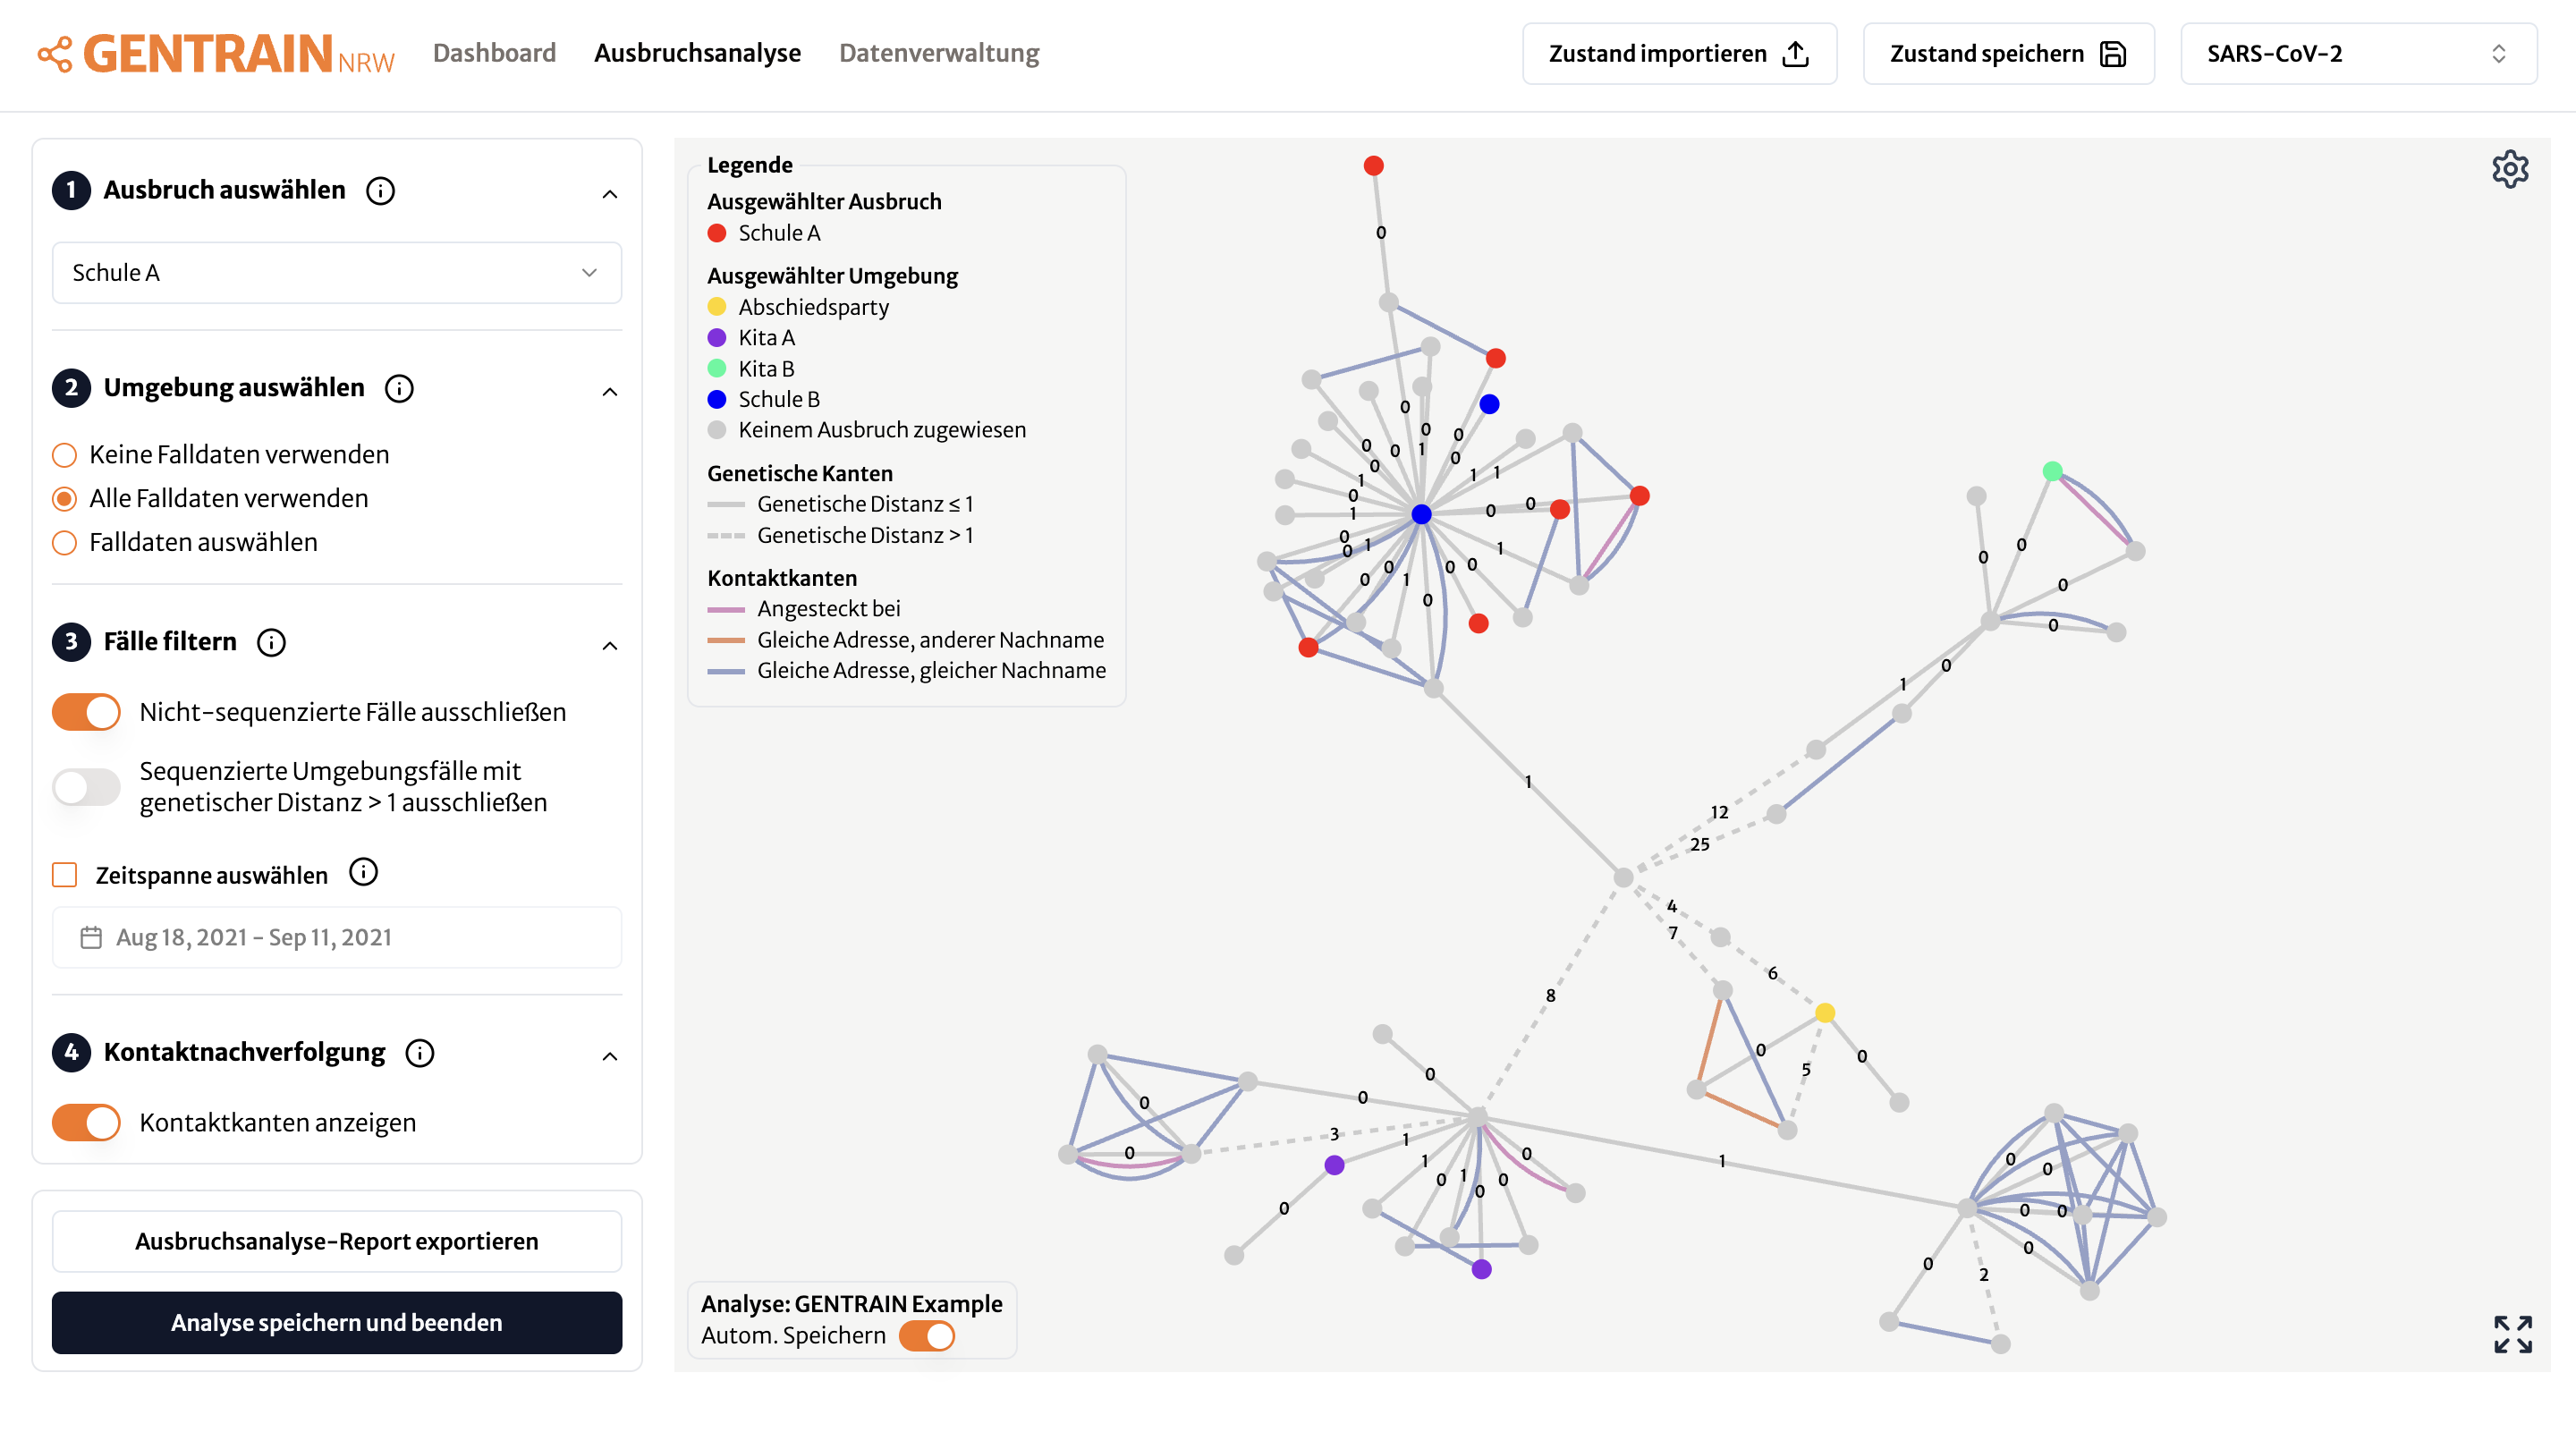
\includegraphics[width=\textwidth]{gentrain}
    \centering
    \caption[Disease outbreak analysis with GENTRAIN]{Disease outbreak analysis with GENTRAIN}
    \label{fig:gentrain}
\end{figure}

GENTRAIN operates within a web browser, where most processes are executed on the client side and data are stored in the local database of the web browser. Initially, the application analyzes imported sequences in terms of the mutations contained (see Section \ref{sec:nextclade}) and persists the results in the local database. This mutation information is a compact representation of the genome sequences and the obligatory information necessary for calculating genetic distance.
The genetic distances between all the sequences imported into the application are calculated based on the detected mutations (see Section \ref{sec:calculation_of_genetic_distances}). Subsequently, the genetic distances are stored in the local database, allowing the generation of an \acrshort{mst} to visualize the outbreak dynamics between the imported sequences. This \acrshort{mst}, which is based on genetics, is extended by contact edges, which represent contact tracing data imported by local public health authorities.
Figure \ref{fig:gentrain} provides a sneak peek at the application. It shows the procedure of a disease outbreak analysis, with genetic distance edges colored gray and contact edges colored differently.

\subsubsection{Nextclade Mutation Calling}
\label{sec:nextclade}
To retrieve mutation information from viral genome sequences, GENTRAIN uses Nextclade, which is a \acrfull{cli} developed by the Nextstrain project. The goal of the project is "to aid epidemiological understanding of pathogen spread and evolution and improve outbreak response" \cite{Nex2}. This section provides a detailed explanation of the Nextclade \acrfull{cli} pipeline with the ultimate goal of understanding how aligned mutation information is obtained from genome sequences. Only the steps relevant to this work are considered.

\begin{description}
    \item[Sequence alignment] The first stage of the pipeline aims to align input sequences, or query sequences, with a specified reference genome pair by pair. Small fragments are identified in which the queries and the reference match exactly. The estimated shift of a query sequence relative to the reference and the number of indels are determined from seed chains that cover sufficient regions of the query sequences. Combining all the resulting estimates produces a sequence of variable length that, with a high probability, covers the entire alignment \cite{Nex3}. The \acrshort{iupac} symbol for gaps is used to mark deleted nucleotides within aligned query sequences \cite{Nex5}. Insertions detected during the alignment are extracted into a separate file for mutation calling later on. If a query sequence is shorter than 100 nucleotides, the alignment is unreliable. Additionally, if a sequence diverges too much from the reference, the alignment may fail because a low number of similar fragments found. Reasons for this include the usage of an inappropriate reference, very low quality query sequences, or query sequences that are too short compared to the reference \cite{Nex3}.
    \item[Mutation calling] The positions at which the query and reference nucleotide sequences differ are identified. Depending on the type of mutation, different notation patterns are applied. For \acrshortpl{snv} the original nucleotide, the reference position and the new nucleotide are reported. For example, a mutation from adenine (\lstinline|A|) to guanine (\lstinline|G|) at reference position \lstinline|300| would be reported as \lstinline|A300G|. Insertions are extracted from the separate file created during sequence alignment. An insertion of the nucleotides \lstinline|ACT| after the reference position \lstinline|22030| would be annotated as \lstinline|22030:ACT|. Deleted regions inside the aligned query sequences are annotated as numeric ranges or reference positions for single nucleotide deletions. A single nucleotide deletion at the reference position \lstinline|300| would be identified as \lstinline|300-301| and a deletion ranging from the reference positions \lstinline|600| to \lstinline|605| would be identified as \lstinline|600-606| \cite{Nex5}. Ambiguous symbols in the \acrshort{iupac} nomenclature are handled differently. The \acrshort{iupac} symbol N is treated like deletions, which means that numerical ranges are specified. Therefore, a series of Ns ranging from the reference positions \lstinline|200| to \lstinline|209| would be annotated as \lstinline|200-210|. All other \acrshort{iupac} symbols, referred to as non-ACGTNs, are reported using both the symbol and the reference position. For example, a \lstinline|Y| at the reference position \lstinline|20021| would result in \lstinline{Y:20021} \cite{Nex5}. Nextclade \acrshort{cli} also counts the number of occurrences of each type of mutation and includes them in the set of results.
    \item[Phylogenetic placement] Nextclade \acrshort{cli} places all query sequences on a phylogenetic tree. For each query sequence, the most similar node in the reference tree is determined based on the mutations in the query and the reference nodes of the reference tree \cite{Nex6}. The reference tree also contains clade annotations that will be used for the next stage of clade assignment.
    \item[Clade assignment] A clade is a group of related genomic sequences. Since the reference tree from the previous stage contains clade annotations, the clade of each query sequence can be determined by identifying the clade of the nearest reference node in the phylogenetic tree. Nextclade \acrshort{cli} includes the associated clade for each query sequence in the set of results \cite{Nex7}.
\end{description}

Nextclade \acrshort{cli} was developed and optimized for large-scale analysis. \cite{Nex1} Although no benchmarking information was found from the Nextstrain project, an yet unpublished article by Ort et al. evaluated the Nextclade CLI runtime for different quantities of avian influenza virus genome sequences. The analysis of 100 sequences took about 0.7 seconds. In addition, Nextclade \acrshort{cli} processed 10,000 sequences in only 20 seconds, corresponding to a processing speed of 500 sequences per second. This allows for the assumption of linear scaling of the Nextclade \acrshort{cli} pipeline \cite{Ort1}.

Although it is only one step in the entire pipeline, subsequent sections will refer to the entire process as Nextclade mutation calling because the results of this step form the basis of the approaches carried out.

\subsubsection{Genetic Distance Calculation}
\label{sec:calculation_of_genetic_distances}
In order to extract differences between two genomes, a pairwise comparison of the sequenced nucleotides must be performed. The GENTRAIN application implements an algorithm originally developed by Alexander Dilthey and Jonas Weber to calculate the genetic distance between genomic sequences. The procedure consists of two phases. In the initial phase, two sequences are reconstructed and aligned with each other on the basis of the mutations detected for the sequence positions of the reference genome. In the subsequent stage, the genetic distance between these reconstructed sequences is incremented in a position-wise manner. This leads to a time complexity of $O(n)$ where n refers to the length of the reference genome. As two iterations are executed during the two phases, the algorithm has a constant factor of $2n$.

Based on the mutation information for each pair of sequences in the local database, both sequences are reconstructed taking into account the nucleotide shifts resulting from the indels. The result is two genome sequences of equal length with aligned nucleotide positions including genomic mutations. To obtain such sequences, the following pairwise nucleotide determination rules are applied for each position of the reference genome, based on the type of mutation present.
\begin{description}
  \item[\acrshort{snv}] The replacing nucleotide is added to the sequence that has an \acrshort{snv} at the current reference position. \acrshortpl{snv} also include ambiguous symbols from the \acrshort{iupac} nomenclature.
  \item[Insertion] The inserted nucleotides are appended to the sequences that have an insertion at the current reference position. In the event that both sequences contain an insertion at the current reference position, they are aligned against each other to identify the most significant overlap of both insertions. The PairwiseAligner of the Biopython package is utilized for the alignment process \cite{Bio1}. This package employs the Smith-Waterman algorithm, a widely recognized approach to find optimal alignments in genome sequences \cite{Bio2}. If one sequence has no insertion at the current position, the amount of inserted positions are filled with gaps.
  \item[Deletion] A gap is added to each sequence that has a deletion at the current reference position. If both sequences have a deletion, the reference position is skipped entirely.
  \item[No mutation] The reference nucleotide for the current position is added to the sequences that do not have a mutation at the current reference position.
\end{description}

Table \ref{table:exemplary_aligned_sequence_reconstruction_result} demonstrates this procedure based on a slice of two exemplary genome sequences. The example shows an ambiguous symbol at reference position 2, an insertion after reference position 3, and a missing symbol at reference position 7 for the first genome. The second genome has an \acrshort{snv} at reference position 5, and a deletion ranging from reference positions 8 to 10. It becomes also clear how sequences are aligned in the presence of indels.

\begin{table}[ht!]
    \caption{Exemplary pairwise sequence reconstruction}
    \centering
    \begin{tabular}{ l | c c c c c c c c c c c c } 
    & \textbf{1} & \textbf{2} & \textbf{3} & & & \textbf{4} & \textbf{5} & \textbf{6} & \textbf{7} & \textbf{8} & \textbf{9} & \textbf{10}\\
    \hline
    \textbf{Reference} & T & A & G & - & - & C & G & T & G & A & G & A \\
    \hline
    \textbf{First genome} & T & Y & G & G & A & C & G & T & N & A & G & A \\
    \hline
    \textbf{Second genome} & T & A & G & - & - & C & A & T & G & - & - & -\\
    \end{tabular}
    \label{table:exemplary_aligned_sequence_reconstruction_result}
\end{table}

Once both sequences were reconstructed and aligned, a genetic distance can be determined. Therefore, for each position where the sequences have a different nucleotide, the genetic distance is increased by 1. Because aligned sequences may be longer than the reference genome sequence, the positions in subsequent algorithmic steps are referred to as alignment positions. Since ambiguous symbols may represent the nucleotide of the other sequence, alignment positions with ambiguous symbols must be examined more closely. In addition, each indel increases the genetic distance by only 1, regardless of the number of nucleotides inserted or deleted. Therefore, the following rules apply, based on the \acrshort{iupac} symbol at the alignment position.

\begin{description}
  \item[Missing symbols] If one of the sequences has N at the current alignment position, the genetic distance is not increased to avoid false negatives.
  \item[Gaps] If a sequence has a gap at the current alignment position, the genetic distance increases only if this sequence had no gap at the previous alignment position.
  \item[Other ambiguous symbols] For other ambiguous symbols, the genetic distance is increased only if the symbol at the current alignment position cannot represent the nucleotide of the other sequence at the current alignment position.
\end{description}

Table \ref{table:exemplary_pairwise_distance_determination_result} shows the increase in the genetic distance between two already reconstructed and aligned sequences per alignment position. At alignment position 9, the genetic distance does not increase due to the presence of an N in the first genome. Since the ambiguous symbol Y cannot stand for nucleotide A according to the \acrshort{iupac} nomenclature, a difference is assumed at alignment position 2. Note that the genetic distance is increased by only 1 for both the insertion between alignment positions 4 and 5 in the first genome and the deletion ranging from alignment positions 10 to 12 in the second genome. 

\begin{table}[ht!]    
    \caption{Exemplary pairwise distance determination}
    \centering
    \begin{tabular}{ l | c c c c c c c c c c c c } 
    & \textbf{1} & \textbf{2} & \textbf{3} & \textbf{4} & \textbf{5} & \textbf{6} & \textbf{7} & \textbf{8} & \textbf{9} & \textbf{10} & \textbf{11} & \textbf{12} \\
    \hline
    \textbf{First genome} & T & Y & G & G & A & C & G & T & N & A & G & A \\
    \hline
    \textbf{Second genome} & T & A & G & - & - & C & A & T & G & - & - & - \\
     \hline
    \textbf{Genetic distance increase} & 0 & 1 & 0 & 1 & 0 & 0 & 1 & 0 & 0 & 1 & 0 & 0 \\
    \end{tabular}
    \label{table:exemplary_pairwise_distance_determination_result}
\end{table}

Sequenced genomes have the characteristic that the quality of sequencing at the beginning and end of the sequence is relatively low. To suppress the influence of these regions on the genetic distance, it is only increased if a specified number of proper symbols has been read from the beginning and the end of both sequences. The proper symbols are all \acrshort{iupac} symbols except Ns and gaps. Once the distances for all combinations of isolates have been calculated, they can be assembled into a distance matrix. Based on this genetic distance matrix, GENTRAIN generates an \acrshort{mst} visualization to facilitate the analysis of disease outbreaks.

\subsection{Related Work}
\label{cha:related_work}
In order to contribute to existing research, the current state of the art in efficient visualizations of large-scale viral outbreak dynamics was examined. 
First, applications designed to support outbreak analysis through user-oriented interfaces were identified. The Nextstrain project was already introduced in Section \ref{sec:nextclade} concerning the Nextclade \acrshort{cli}, which is used by GENTRAIN to identify mutations in genomes. In addition to the \acrshort{cli}, Nextstrain provides a user-oriented web application that visualizes outbreak dynamics based on genome sequences \cite{Nex9}. Like Nextclade \acrshort{cli}, the web application compares sequences against a reference genome. The relationships are then displayed using phylogenetic trees, which are also used by the Nextclade \acrshort{cli} to distinguish clades. However, the application crashed while processing 5,000 sequences, suggesting that it is not optimized for large-scale analysis. Microreact is another example of a user-oriented application that supports outbreak analysis. In an article, Argimón et al. described the motivations and underlying technical concepts behind the application \cite{Mic1}. The application allows users to visualize genome sequence relationships using different types of tree-based graphs, as trees are the most well-established tool for analyzing genomic dynamics. It was developed in response to the transition in genomics from sequencing a few representatives to sequencing large numbers of populations. This allows for more detailed analyses of highly similar genomes, which should be accessible to users with different levels of expertise. 
The authors also mentioned the challenges resulting from large-scale datasets. However, they addressed these issues by emphasizing the need for research on alternative visualizations for such scenarios. Therefore, in addition to using visualizations that represent seasonal and geographic contexts, the author proposed a "high-level clustering of tree branches with subsequent expansion of nodes of interest" \cite{Mic1}. It is also important to mention that Microreact only processes graphs that have already been constructed, and therefore does not calculate genetic distance matrices itself.

These applications focus on genetic-based outbreak analysis that also considers seasonal and geographic contexts. As described in Section \ref{sec:viral_outbreak_analysis}, genome sequence information can be used in a way to support traditional epidemiology, a procedure that was introduced as \acrshort{igs}. Walker et al. conducted research on the relationship between genome isolates and the potential of \acrshort{igs}, demonstrating the procedure using miscellaneous contact tracing and genetic data sets in urban scenarios \cite{Wal1}. The authors identified links between several independent outbreak scenarios, some of which crossed national borders.
Furthermore, Bludau et al. analyzed acceptance criteria and state of the art in the use of \acrshort{igs} by local public health authorities in Germany \cite{Blu1}. Their investigation showed that the degree to which different local public health authorities use \acrshort{igs} varies greatly. They emphasized the potential of \acrshort{igs} for disease surveillance by supporting outbreak analysis and investigation of transmission chains. It was also mentioned that the required sequence availability is highly dependent on the objectives of the local public health authorities. Retrospective analyses can be performed with a smaller number of available sequences, but real-time outbreak analyses require higher sequencing throughput. In general, the authors defined the goal of simultaneously improving access to genome analysis for non-specialists and expanding the genomic expertise of local public health authorities in Germany.
Furthermore, a paper by Hanke et al. discussed the potential of \acrshort{igs} for interrupting HIV transmission dynamics \cite{Han1}. The paper focused on the impact of crises such as the SARS-CoV-2 pandemic and the war in Ukraine, which has led to massive refugee movements. They predicted that a "full automation of laboratory and data analysis processes [...] will enable HIV-\acrshort{igs} to enhance efficiency, effectiveness and accuracy of the entire HIV operational workflow".

These findings on the relevance of \acrshort{igs} emphasizes the need for user-oriented applications that address \acrshort{igs}. They also highlight the necessity of making these applications capable of handling large-scale datasets, especially for retrospective analysis. Therefore, approaches for comparing genome sequences were explored, while focusing on their applicability to large-scale datasets.
First, sequence comparison should be separated into alignment-free and alignment-based approaches. The first group yields rapid results, while the latter focuses on achieving a higher accuracy \cite{Lei1}. One prominent method of representing genome sequences using alignment-free methods is the use of k-mers \cite{Lei1}. These are based on the frequencies of words consisting of nucleotide sequences and are comparable to n-grams, a concept widely used in natural language processing. However, since the GENTRAIN algorithm is based on the mutation information of genome sequences that were first aligned by the Nextclade \acrshort{cli}, this research focuses more on alignment-based sequence comparison. Applications such as GENTRAIN aim to extract very accurate distances from genome sequences because low distances are responsible for the identification of infection chains.

The Hamming distance indicates pairwise genetic distance by measuring the number of nucleotide differences between two aligned sequences \cite{Hos1}. Assuming error-free sequencing and no ambiguous symbols, this would strictly underestimate the distances calculated by GENTRAIN. In 2021, Grabowski and Kowalski published an article that addressed the quadratic scaling problem in Hamming distance matrices \cite{Gra1}. Therefore, the calculation of relevant Hamming distances was performed using variant methods to identify relevant candidates. Most of these methods identified relevant candidates by filtering out sequence pairs that exhibit a genetic distance of more than a specified distance threshold. In general, the algorithms applied showed about an order of magnitude faster than complete matrix calculations, demonstrating the potential for efficiency improvements in calculating selective genetic distance matrices.

Another procedure that has been widely explored in the field of genomic sequence comparison is \acrfull{anns}. The objective is to find nearest neighbors in high-dimensional datasets for which an accurate nearest neighbor search is no longer efficient while preserving accuracy to the greatest extent possible \cite{Wan1}. \acrshort{anns} algorithms can be categorized as graph-based, partition-based, quantization-based, and hash-based methods \cite{Wan1}. Each of these methods employs a distinct procedure to approximate the nearest neighbors. Partition-based \acrshort{anns} divides the high-dimensional space into multiple regions. Then, the nearest neighbors are searched in the region of the query or nearby regions \cite{Li1}. In quantization-based \acrshort{anns}, data vectors are divided into multiple subvectors to enable a more efficient search based on compact representations using the centroid indices identified for each subvector \cite{Pen1}. When using hash-based \acrshort{anns}, data are transformed into low-dimensional representations, called hashes, to efficiently identify similarities on a smaller scale \cite{Li1}. Graph-based \acrshort{anns} relies on the construction of a proximity graph, which is then traversed to find the closest nodes for a given query \cite{Wan1}.

In the field of genomic sequence comparison, hash-based \acrshort{anns} is widely used, while other ANNS categories are less represented in genomic sequence comparison. Several related studies have applied the so-called \acrfull{lsh} to identify similar genome sequences. Although the original purpose of hashing is to find hashes to minimize collisions, \acrshort{lsh} does the opposite. The observed inputs are sorted into so-called \acrshort{lsh} buckets, where the colliding hashes are placed in the same bucket. The OMH method \cite{Mar2}, developed by Marçais et al., approaches calculating the edit distance using unaligned sequences, while also taking the relative order of k-mers into account. This method achieves a low number of false negatives while reducing the required runtime. However, this work overcomes this challenge by using already aligned sequence information from Nextclade mutation calling. Other studies focusing on the identification of similar genome sequences in large-scale datasets aim to strike a balance between false positives and false negatives \cite{Mus1, Wan2}. Therefore, Nimrah Mustafa proposes an LSH approach based on an AND/OR construction of hash functions, where the OR component serves to reduce false negatives and the AND component serves to reduce false positives \cite{Mus1}. In 2024, Zhao et al. introduced the GSEARCH method that combines k-mer hashing of sequences with a graph-based \acrshort{anns} method to identify highly similar sequences in very large genome datasets \cite{Zha2}.
The genetic relatedness of the sequences was determined using the Jaccard distance exhibited from the hash representations of the sequences. Upon these distances an \acrshort{hnsw} (\acrlong{hnsw}) graph was constructed to avoid quadratic scaling of distance calculation. In an \acrshort{hnsw} graph, a query node is inserted by repeatedly comparing the query distance to a currently focused node with the distances to its neighboring nodes until the nearest neighbors of the query are found. This means that the query does not need to be compared to every node in the graph. To further improve time complexity, hierarchical levels are added to the graph, enabling a search to first be conducted within a coarser set of nodes before the degree of detail is incrementally being increased. This graph can be updated and expanded with new queries, thus avoiding the need to rebuild the graph. A more detailed explanation of the procedure can be found in the fundamental article on \acrshort{hnsw} graphs by Malkov and Yashunin \cite{Mal1}. GSEARCH exhibited a time complexity of $O(log n)$, overcoming the quadratic scaling of genetic distance matrices, and producing promising results for datasets comprising highly similar genomes \cite{Zha2}. Therefore, the application of \acrshort{hnsw} could be sufficient to compare genomes of the same virus, as in this work.

Several studies have been found on how to calculate genetic distances more efficiently and identify similar genomes in large datasets \cite{Gra1,Mar2,Zha2,Mus1}. However, a research gap has been identified regarding the effects of these optimizations on visualizations for outbreak analysis. Furthermore, current research primarily focuses on phylogenetic relations, representing a broader examination of lineages than the fine-grained analysis of direct infection chains. The latter forms the foundation for \acrshort{igs}, a topic that has been frequently discussed in research due to the SARS-CoV-2 pandemic, emphasizing its relevance in the near future \cite{Wal1, Wal2, Blu1, Han1}. User-oriented applications such as Nextstrain and Microreact partially cover \acrshort{igs} by combining genetic data with seasonal and geographic attributes. However, to the best of the authors' knowledge, GENTRAIN is the only user-oriented application that provides graph visualizations of traditional epidemiological connections, such as those collected by local public health authorities, as well as genetic relatedness.
    \clearpage
    \section{Methodology}
\label{cha:methodology}
This chapter describes the methodological concepts applied to answer the research question in a scientific way to ensure reproducibility. The data sources selected for this study are introduced and the data preparation process is outlined. Furthermore, the approaches carried out to minimize the computational runtime involved in generating \acrshortpl{mst} based on the GENTRAIN algorithm are delineated. Finally, the implementation and evaluation procedures are described. All corresponding source code is bundled into a Python module, which can be found in the accompanying GitHub repository \cite{Git1}.

\subsection{Data Understanding and Preparation}
In addition to innovative technical approaches to epidemiology, containing the SARS-CoV-2 pandemic has required countries to adjust their legal. For example, Germany introduced an ordinance for the surveillance of SARS-CoV-2, which included genome sequencing obligations \cite{Bmg1}. Sequencing laboratories were required to send sequenced genomes to the \acrfull{rki}, which is the leading biomedical research institution of the German federal government.
Thus, the \acrshort{rki} has compiled a comprehensive SARS-CoV-2 genome sequence dataset ("SARS-CoV-2 Sequenzdaten aus Deutschland"), which is freely accessible and regularly updated. 

Genome sequences are provided as a file containing unique ids along with the corresponding genome sequences. As expected for SARS-CoV-2 genomes, the sequences are around 30,000 nucleotides long. Nextclade was used to perform a sequence analysis on all sequences. As explained in Section \ref{sec:nextclade}, this also involves aligning all sequences with a reference genome. The Wuhan-Hu-1/2019 (MN908947) sequence \cite{Wu1} was used, which is the default SARS-CoV-2 reference in Nextclade. Lists of \acrshortpl{snv}, insertions and deletions, as well as ambiguous \acrshort{iupac} symbols, were obtained for each sequence. The number of mutations of each type and the resulting clade from the clade assignment stage (described in Section \ref{sec:nextclade}) were collected. The lineage of sequences is further distinguished by the inclusion of sublineages defined by the PANGO consortium \cite{Pan1}.

\begin{table}[ht!]
    \caption{Dataset fields and sources}
    \centering
    \small
    \begin{tabularx}{\textwidth}{l|l|X}
    Name & Source & Description \\
    \hline
    \hline
    \ttfamily{igs\_id} & \acrshort{rki} & Unique identifier to map metadata with genome sequences. \\
    \hline
    \ttfamily{date\_of\_sampling} & \acrshort{rki} & Date on which the sample was collected by the primary diagnostic laboratory. \\
    \hline
    \ttfamily{sequencing\_platform} & \acrshort{rki} & Platform technology used for sequencing. The dataset consists of following options which were also discussed in Section \ref{sec:genome_sequencing_technologies}: ILLUMINA, 
    OXFORD\_NANOPORE, ION\_TORRENT. \\
    \hline
    \ttfamily{variant} & \acrshort{rki} & Defined by the \acrshort{who}. The most prevalent variants for SARS-CoV-2 viruses are Alpha, Delta and Omicron. \\
    \hline
    \ttfamily{lab\_postal\_code} & \acrshort{rki} & Postal code of the primary diagnostic laboratory that collected the corresponding sample. \\
    \hline
    \ttfamily{\acrshortpl{snv}} & Nextstrain & List of detected \acrshortpl{snv} in a genome sequence, along with their corresponding reference position. \\
    \hline
    \ttfamily{insertions} & Nextstrain & List of the symbols inserted into a genome sequence, along with their corresponding reference positions. \\
    \hline
    \ttfamily{deletions} & Nextstrain & List of ranges of reference positions in a genome sequence at which a deletion was detected. \\
    \hline
    \ttfamily{missing} & Nextstrain & List of ranges of reference positions in a genome sequence at which an N was detected. \\
    \hline
    \ttfamily{non\_acgtns} & Nextstrain & List of symbols that are not one of the common nucleotides or N, along with their corresponding reference position. \\
    \hline
    \ttfamily{total\_\acrshortpl{snv}} & Nextstrain & Total number of detected \acrshortpl{snv} in a genome sequence. \\
    \hline
    \ttfamily{total\_insertions} & Nextstrain & Total number of detected insertions in a genome sequence. \\
    \hline
    \ttfamily{total\_deletions} & Nextstrain & Total number of detected deletions in a genome sequence. \\
    \hline
    \ttfamily{total\_missing} & Nextstrain & Total number of Ns in a genome sequence. \\
    \hline
    \ttfamily{total\_acgtns} & Nextstrain & Total number of symbols that are not one of the common nucleotides or N. \\
    \hline
    \ttfamily{clade} & Nextstrain & Lineage association identified on the phylogenetic tree during Nextclade analysis. \\
    \hline
    \ttfamily{sublineage} & Nextstrain & Fine-grained lineage association defined by the PANGO consortium \cite{Pan1}. \\
    \hline
    \ttfamily{lab\_city} & \acrshort{godi} & City name of the primary diagnostic laboratory that collected the corresponding sample. \\
    \hline
    \ttfamily{lab\_federal\_state} & \acrshort{godi} & Federal state name of the primary diagnostic laboratory that collected the corresponding sample. \\
    \end{tabularx}
    \label{table:rki_metadata}
\end{table}

Finally, the original sequences from the dataset were dropped as further processing was deemed unnecessary. To evaluate the runtime of the Nextclade mutation calling process, the determination was carried out independently for different numbers of sequences. The resulting runtime in seconds was averaged across multiple executions of the process.

In addition to the genome sequences themselves, the \acrshort{rki} dataset includes metadata which provides further context for each sequence. For this work, the postal code of the primary diagnostic laboratories that collected the samples, the dates of sampling, the sequencing technologies used, and the virus variants defined by the \acrshort{who} were used.
The postal codes of the primary diagnostic laboratories were mapped with the names of cities and federal states in Germany. Therefore, the location dataset for Germany from the \acrfull{godi} \cite{Glo1} was used. Table \ref{table:rki_metadata} provides a list of the combined dataset and a description of each field.

After constructing the dataset, it was analyzed in order to understand the data in terms of its characteristics and limitations. Therefore, the seasonal and geographic distribution of the sequences was observed. In addition, genetic aspects such as variant and clade distribution, as well as mutation dynamics, were examined.

\subsubsection{Seasonal and Geographic Data Aggregation}
\label{sec:seasonal_and_geographical_data_aggregation}
As the dataset provides an extensive picture of the SARS-CoV-2 pandemic, it was not feasible to incorporate all available data. For a virus that exhibits dynamic mutation behavior, such as SARS-CoV-2, the results obtained can vary significantly depending on the data observed. Consequently, data aggregates were generated according to the \acrshort{who} definition of outbreaks by seasonal periods and geographic areas. Seasonal periods were delineated by intervals of a week, a month, and a year, while the geographic span was represented by the municipal, federal state, and the country.

In order to ensure that the aggregates adequately represent diverse outbreak scenarios, the mutation diversity and infection density were elaborated. Mutation diversity was observed by comparing the number of present clades per aggregate. In contrast, several definitions were introduced to analyze infection density within the aggregates.
For a genetic distance matrix $D \in \mathbb{R}^{N \times N}$ with $D = D^T$ and $N$ being the amount of sequences considered, the genetic distance between sequences $i$ and $j $ is defined as $D_{ij}$ and the total distance amount $|D|$ corresponds to $\binom{N}{2}$. According to the replication behavior of the SARS-CoV-2 virus, as explained in Section \ref{sec:viral_mutation_dynamics_and_isolate_relatedness}, an infection is assumed between the sequences $i$ and $j$ if $D_{ij} < 2$ for $i \neq j$. This does not imply that an infection and therefore a direct transmission must have occurred between the disease cases associated with these sequences. It is more an indicator that a direct transmission could have occurred and that the investigation of these cases is relevant to understand the infection chains of the observed scenario. Nevertheless, to ensure consistent terminology throughout this work, these genetic distances will be referred to as infections in the context of SARS-CoV-2. The amount of infections is expressed as:
$$I = \sum_{1 \le i < j \le n} \mathbf{1}_{\{D_{ij} < 2\}}$$

To gain an understanding of how these infections are distributed through complete distance matrices, the infection rate is defined as the proportion of $I$ in the total distance amount $D$. To investigate these parameters, it was necessary to calculate complete genetic distance matrices. As this calculation scales quadratically with the number of sequences considered, the aggregates were downsampled to a size of 1,250 sequences. During the sampling process, the geographic and seasonal sequence distribution was preserved to maintain aggregate characteristics. This preservation included the representation of dates (or months for aggregates comprising long seasonal periods), and cities (for the federal state level) or federal states (for the country level). The genetic distance matrices were then calculated using the GENTRAIN algorithm described in Section \ref{sec:calculation_of_genetic_distances}.

\subsubsection{Mutation Encoding}
\label{sec:mutation_encoding}
In order to efficiently approximate genetic distances, it was necessary first to create sparse numeric representations of the mutation information. As previously described, the dataset comprises mutation information for sequences, expressed in the form of Nextclade mutation strings (see Section \ref{sec:nextclade}). The simplest algorithmic approach to processing these data would be to treat each mutation string as a word and build a vocabulary that can be represented numerically using one-hot encodings. These represent inputs as binary vectors, where each position in a vector indicates whether a particular word from the vocabulary is present (1) or absent (0) for each input in the dataset. However, this would make the encoding structure very inflexible, which would complicate any subsequent filtering process based on the reference position and mutation type. Consequently, a position-based encoding approach was implemented.

When \acrshortpl{snv} and deletions are taken into account alone, the length of this encoding could be represented by the length of the reference genome. However, in order to ensure forward-looking compatibility with other viruses, it was essential not only to respect \acrshortpl{snv} and deletions but also insertions. Including insertions means that the shared encoding length must be extended, so that resulting encoding vectors are longer than the reference genome sequence. Nextclade describes insertions by indicating at which reference position the inserted characters are placed after. To keep the sequence vectors aligned, all reference positions subsequent to the insertion reference position need to be projected to a higher encoding position. Since the GENTRAIN distance calculation increases the distance for consecutive gaps in one sequence only by 1 (see \ref{sec:calculation_of_genetic_distances}), this projection value is limited to 1 per reference position. More strict algorithms may be approximated using greater projection values.

During the mutation encoding procedure, the projected reference positions are recorded in a mapping object. The keys of this object represent the original reference positions and the values represent the resulting encoding positions.
Next, a vector of the encoding length is initialized for each sequence considered. These vectors are then populated exclusively with zeros, which initially represent totally unmutated genomes, serving as the basis for the further encoding process.
In the following procedure, for each reference position that is processed, it undergoes a conversion into its corresponding encoding position from the mapping object. For each \acrshort{snv}, insertion and deletion per sequence, zeros at the encoding position are then replaced by ones, thereby representing a mutated position. In the event of an insertion or a deletion that is more than one position, only the starting positions of the affected area will be marked as mutated. This is done to ensure that the handling of the gaps in the GENTRAIN distance calculation is adequately addressed. For insertions, this starting position is determined by incrementing the defined reference position from the Nextclade mutation string by one to find the actual position of the nucleotide insertion.

The resulting vectors provide information on the positions in which the sequences underwent mutation (1) and those in which they did not (0). Visualizations of outbreak dynamics, and therefore infection chains, focus exclusively on differences between genomes. Therefore, all encoding positions that do not show mutations for any sequence vector can be safely omitted from the encoding. Consequently, the encoding is reduced to the maximum amount of information necessary to obtain genetic distances, under the assumption that the sequences would be perfectly sequenced. However, this assumption can be invalidated by the recent progress of sequencing technology, as discussed in Section \ref{sec:genome_sequencing_technologies}.

Given that GENTRAIN avoids overestimating genetic distances, which could occur due to the possible ambiguity of sequence symbols, the way ambiguous symbols are handled must also be reflected. The GENTRAIN distance calculation handles ambiguous symbols from the \acrshort{iupac} nucleotide nomenclature differently. In the case of the presence of a missing symbol, the distance will not increase at all. This helps prevent the accounting of false positive detections of nucleotide differences. Other ambiguous symbols are mapped against their \acrshort{iupac} nucleotide assignments before deciding on an increase in genetic distance. This behavior cannot be addressed in a straightforward manner using vector encodings. To solve this issue, positions are filtered from the encoding that account for a high number of missing symbols throughout the sequences under consideration. 
Therefore, all missing positions are collected by sequence and then concatenated into a single list. From this list, the number of occurrences of each missing position is counted. Missing positions that occur more frequently than a defined threshold were marked for exclusion from the encoding. In this work, this threshold is set to 5\% of the total number of sequences considered to avoid excluding an excessive number of positions. Since the encoding is designed to approximate the GENTRAIN distance calculation, it was preferable to underestimate the genetic distances rather than overestimate them. Significant overestimation would be the result of ignoring missing positions or choosing a threshold that is too low.
The filtering procedure for missing high-frequency positions was designated as \acrfull{nff}, which has the positive side effect of reducing the size of the encoding. 

A second applied filter was labeled \acrfull{snvff}. Its purpose was to further shorten the encodings, while retaining the positions of the characteristic \acrshortpl{snv} of the resulting \acrshort{mst} visualizations. Therefore, \acrshortpl{mst} and their corresponding Louvain communities of various data aggregates were analyzed in terms of \acrshortpl{snv} that occur. For each detected community of an \acrshort{mst} the \acrshortpl{snv} from all contained sequences were collected, while only a unique entry per \acrshort{snv} was maintained. The characteristic \acrshortpl{snv} that appear exclusively within their respective communities were then identified. For each characteristic \acrshort{snv} the number of occurrences in the corresponding community sequences was observed. Based on the minimum and maximum observed occurrences, the \acrshortpl{snv} that occurred significantly more frequently or less frequently were assumed to be uncharacteristic and not considered further. While \acrshort{snvff} significantly minimizes the length of the encoding, it also reduces the information gain. Therefore, different encoding approaches (without filtering, with \acrshort{nff}, with \acrshort{nff} \& \acrshort{snvff}) were evaluated.

\subsection{Implementation}
\label{sec:implementation}
The GENTRAIN distance calculation is susceptible to two aspects of time complexity. One concern is the calculation of the genetic distance itself, which is designed to yield highly precise results in order to accurately reflect infection chains. The second issue concerns the nature of quadratic scaling in distance matrices as the number of sequences increases. In the present work, the first issue is addressed by reducing the observed genomic information of the algorithm to the minimum necessary. To reduce the factor of quadratic scaling, the most relevant calculation candidates to generate adequate \acrshortpl{mst} are identified based on approximate genetic distance matrices. Finally, this work addresses large-scale scenarios in which the calculation of approximate genetic distance matrices through the distance matrix approximation reaches its limit. For these cases, an approach based on approximate nearest neighbor search is proposed to identify relevant candidates and calculate sparse distance matrices.

\subsubsection{Modification of the GENTRAIN Algorithm}
\label{sec:optimization_of_the_gentrain_algorithm}
The algorithm introduced in Section \ref{sec:calculation_of_genetic_distances} calculates the genetic distance $d(s_1,s_2)$ for the genome sequences $s_1$ and $s_2$.
Since the runtime of calculations is crucial especially for large-scale scenarios, this work first aims to speed up the algorithm itself. Currently, the algorithm must first iterate through all positions in the reference genome to reconstruct and align two genome sequences. Subsequently, a second iteration is necessary to potentially increase the genetic distance per reference position. However, iterating the entire genome a second time instead of just the mutated positions might have a tremendous effect on algorithmic runtime, especially when considering large-scale sequence datasets. The question of whether the advantages of iterating all reference positions twice justify the effects on runtime is questionable. This is due to the fact that the presence of the same symbols in both observed sequences, as well as the presence of a missing symbol in one sequence, does not result in an increase in genetic distance. However, the GENTRAIN algorithm requires a position-wise observation to increase distance only if the necessary number of proper symbols was seen. Furthermore, indels should only increase genetic distance by one. To achieve this, unmutated positions between two subsequent indels must be taken into account.

Two measures were taken to optimize the algorithm with regard to the described issues. First, the algorithm was adjusted to only consider positions in the reference genome that contain a mutation in one of the sequences during sequence reconstruction. Furthermore, reference positions that contain missing symbols in either sequence are excluded from the reconstructed sequences, as these are bypassed in the subsequent stage. Consequently, since the second iteration does not iterate the entirety of the reference genome, the proper symbols that were observed cannot be evaluated. In order to still ensure the observation of exclusively qualitative genome parts, mutated positions are only considered if the position falls within the range between the starting and ending positions of the alignment, as specified by Nextclade. Figure \ref{fig:algorithm_comparison} demonstrates the adjustments to the original GENTRAIN algorithm. Both algorithms perform the first iteration to reconstruct and align sequences over a comparable range of reference positions. However, the second iteration procedure to iteratively determine the genetic distance is minimized for the modified algorithm.

\begin{figure}[ht]
\centering    
\tikzset{
    startstop/.style={rectangle, rounded corners, minimum width=2cm, minimum height=0.8cm, text width=2cm, text centered, draw=black, fill=white},
    process/.style={rectangle, minimum width=3cm, text width=6.5cm, minimum height=1cm, text centered, draw=black, fill=white},
    arrow/.style={thick,->,>=stealth},
    io/.style={trapezium, trapezium left angle=70, trapezium right angle=110, text width=6cm, minimum height=1cm, text centered, draw=black, fill=white}
}
  \begin{subfigure}[b]{0.49\textwidth}
    \begin{tikzpicture}[every node/.style={font=\footnotesize}, node distance=2.1cm]
        
        \node (start) [startstop] {Start};
        \node (mutations) [io, below=0.5cm of start] {Nextclade mutation calling results for two genomes};
        \node (loop1) [process, below of=mutations] {\underline{Pairwise sequence reconstruction}\\\vspace{0.3em}
        Iterates reference genome\\
        \vspace{0.3em}
          \hrule
        \vspace{0.3em}
        Considers all symbols during sequence reconstruction};
        \node (sequences) [io, below of=loop1] {Sequences of unmutated and mutated reference positions};
        \node (loop2) [process, below of=sequences] {\underline{Pairwise distance determination}\\\vspace{0.3em}
        Iterates sequences of unmutated and mutated reference positions\\
        \vspace{0.3em}
          \hrule
        \vspace{0.3em}
        Assesses proper symbols seen};
        \node (distance) [io, below of=loop2] {Genetic distance between the two genomes};
        \node (end) [startstop, below=0.5cm of distance] {End};
        
        \draw [arrow] (start) -- (mutations);
        \draw [arrow] (mutations) -- (loop1);
        \draw [arrow] (loop1) -- (sequences);
        \draw [arrow] (sequences) -- (loop2);
        \draw [arrow] (loop2) -- (distance);
        \draw [arrow] (distance) -- (end);
        
        \end{tikzpicture}
    \caption*{(a) GENTRAIN algorithm}
  \end{subfigure}
  \begin{subfigure}[b]{0.49\textwidth}
       \begin{tikzpicture}[every node/.style={font=\footnotesize}, node distance=2.1cm]
        
        \node (start) [startstop] {Start};
        \node (mutations) [io, below=0.5cm of start] {Nextclade mutation calling results for two genomes};
        \node (loop1) [process, below of = mutations] {\underline{Pairwise sequence reconstruction}\\\vspace{0.3em}
        Iterates reference genome \textbf{within alignment ranges}\\
        \vspace{0.3em}
          \hrule
        \vspace{0.3em}
        \textbf{Ignores equal and missing symbols} during sequence reconstruction};
        \node (sequences) [io, below of=loop1] {Sequences of \textbf{deviating mutations except missing symbols}};
        \node (loop2) [process, below of=sequences] {\underline{Pairwise distance determination}\\\vspace{0.3em}
        Iterates sequences of \textbf{deviating mutations except missing symbols}\\
        \vspace{0.3em}
          \hrule
        \vspace{0.3em}
        \textbf{Ignores} proper symbols seen};
        \node (distance) [io, below of=loop2] {Genetic distance between the two genomes};
        \node (end) [startstop, below=0.5cm of distance] {End};
        
        \draw [arrow] (start) -- (mutations);
        \draw [arrow] (mutations) -- (loop1);
        \draw [arrow] (loop1) -- (sequences);
        \draw [arrow] (sequences) -- (loop2);
        \draw [arrow] (loop2) -- (distance);
        \draw [arrow] (distance) -- (end);
        
        \end{tikzpicture}
    \caption*{(b) Modified algorithm}
  \end{subfigure}
\caption[Comparison of the GENTRAIN algorithm and the modified version]{Comparison of the GENTRAIN algorithm and the modified version. The flowcharts focus on the modifications to the GENTRAIN algorithm, which are in bold. Trapezoids represent inputs and outputs, and rectangles represent processes.}
\label{fig:algorithm_comparison}
\end{figure}

Both implementations show a time complexity of $O(n)$ with two iterations being performed. However, in the GENTRAIN implementation, for the second iteration $n$ refers to at least the length of the reference genome, while in the modified algorithm, $n$ refers to the sum of unique mutation positions in both sequences. Although this does not dramatically affect the actual runtime for smaller sequence datasets, it should result in an immense decrease in runtime on a larger scale. In the worst-case scenario, $n$ is equal for both implementations if at least one mutation is found at each reference position. Since this is not a realistic scenario, one could assume that the algorithmic changes truly optimize the algorithm in terms of runtime.

\subsubsection{Complete Candidate Search}
\label{sec:accurate_candidate_search}
Approximate genetic distance matrices were used to identify the most relevant candidates for an exact calculation of genetic distance. The objective was to calculate sparse matrices of exact genetic distances to reduce the total algorithmic runtime. Sparse matrices are also beneficial for the \acrshort{mst} generation and memory purposes. This procedure was designated as \acrfull{ccs}, as the candidates are identified based on complete matrices resulting from the genetic distance approximation. 

To approximate the genetic distance ${d}(s_1,s_2)$ for the sequences $s_1$ and $s_2$, the sum of a position-wise exclusive OR (XOR) is calculated between the mutation encoding vectors $m_1$ and $m_2$. Essentially, the Hamming distance is examined, which corresponds to the number of different values in both encoding vectors.

$$\tilde{d}(s_1, s_2) = \tilde{d}(m_1, m_2) = \sum_{i=1}^{L_{encoding}} m_{1_i} \oplus m_{2_i}$$

A single genetic distance approximation has a time complexity of $O(n)$ with $n$ referring to the length of the encoding. However, when calculating an approximate genetic distance matrix, a time complexity of $O(n^2)$ is present. Although this approach implies quadratic scaling, it is anticipated that the reduced runtime of a single genetic distance determination will be particularly advantageous for large datasets. Given that the encoding length depends on the number of mutations present in the sequences, it must be assumed that both parameters that affect the runtime increase with the number of sequences. Consequently, the runtime for data aggregates with varying sequence counts was evaluated. Assuming there are no ambiguous symbols, this approximation would consistently underestimate the GENTRAIN genetic distance results. However, overestimation cannot be definitively ruled out, since missing symbols are only observed globally through position filtering and not at the pairwise level.

The approximate genetic distance matrices were then used for relevant candidate search. Different search strategies were developed based on the question of whether finding only the lowest genetic distances (depth search) or finding a broad representation of sequences (breadth search) is more important to generate adequate \acrshortpl{mst} based on sparse genetic distance matrices.
Both approaches first calculate the approximate genetic distances between all sequences considered, which are then sorted in ascending order. A dictionary is created in which the values represent the sorted approximate distances and the keys represent tuples of the two corresponding sequence identifiers. Furthermore, a limit for the remaining number of calculations $n_{calc}$ is expressed as $r_{calc}*|D|$, which is driven by the forced remaining calculation rate $r_{calc}$. The two methods then proceed differently:

\begin{description}
    \item[Depth search] The keys of the dictionary are extracted as a list, which is then cut to a length of $n_{calc}$. This retains the tuples of sequence pairs with the lowest approximate distances. Candidate pairs are extracted directly from this list to identify the sequences that are most similar on the basis of approximate genetic distance.
    \item[Breadth search] The list of sequence pairs sorted by approximate genetic distances is iterated, and candidate pairs are extracted subsequently. Therefore, a candidate entry is added for both sequences if the number of candidates for $s_1$ did not reach the limit of maximum candidates per sequence. This limit is derived from $n_{calc}$ divided by the number of sequences considered.
\end{description}

Sparse genetic distance matrices and corresponding \acrshortpl{mst} for several seasonal and geographic aggregates were generated for both approaches. The aggregates considered were determined based on the observations resulting from the analysis introduced in Section \ref{sec:seasonal_and_geographical_data_aggregation}. Furthermore, data aggregates of different sample sizes were considered because sequence density could affect visualization of outbreak scenarios. The determined sample sizes were 1,250, 2,500, and 5,000, which appears plausible in terms of sequence availability during a pandemic. Complete distance matrices using the modified algorithm were computable in a reasonable amount of time on regular computers for these dimensions, enabling the evaluation against complete reference matrices. The evaluation of results was performed taking the calculation rates of 0.05, 0.1, 0.15 and 0.2 into account. These rates were chosen to significantly reduce the necessary calculations and determine the minimum number of calculations recommended to achieve adequate visualizations for different seasonal and geographic scenarios. 

\subsubsection{Approximate Candidate Search}
\label{sec:approximate_candidate_search}

The \acrshort{ccs} approach relies on computing an approximate but complete genetic distance matrix. Therefore, it does not address the general issue of quadratic scaling, which reveals the limiting factor of the number of sequences that can be considered.
Thus, an \acrfull{acs} approach based on \acrshort{anns} was also evaluated. As the present work focuses on finding adequate methods to efficiently generate adequate \acrshort{mst} visualizations, the \acrshort{acs} approach was implemented based on the findings of Nimrah Mustafa's work on \acrshort{lsh} for big data analytics (see Section \ref{cha:related_work}). The following definitions adhere strictly to Mustafa's work, applying it to the circumstances of this work. The proposed method was labeled AND/OR-\acrshort{lsh}, which associates sequences with so-called \acrshort{lsh} buckets. All sequence pairs associated with the same bucket are treated as relevant for the calculation of genetic distances. Therefore, a hash family $\mathcal{H}$ consisting of $n$ hash functions is defined as $\mathcal{H} = \{h_i: 1 \leq i \leq n\}$ and a hash function $h$ is defined as $h: \{0,1\}^n \rightarrow \{0,1\}$. For a mutation encoding $m = (m_1,m_2,...,m_n)$, the hash function $h_i$ would return the value of the $i$th position in $m$.
To minimize false positives, an AND construction of a set of $r$ hash functions is employed. This yields a derived hash function:
$$h_k'(m_1) = h_k'(m_2) \Leftrightarrow h_{k1}(m_1) = h_{k1}(m_2) \land h_{k2}(m_1) = h_{k2}(m_2) \land ... \land h_{kr}(m_1) = h_{kr}(m_2) $$
According to this definition, two sequences are associated with the same \acrshort{lsh} bucket only if $h_k' = 1$, which means that all the hash functions for both sequences return the same value. Mustafa also suggests an OR construction of $b$ derived hash functions to minimize false negatives.
$$h''(m_1) = h''(m_2) \Leftrightarrow h_{1}'(m_1) = h_{1}'(m_2) \lor h_{2}'(m_1) = h_{2}'(m_2) \lor ... \lor h_{b}'(m_1) = h_{b}'(m_2) $$
Sequences are now associated with the same \acrshort{lsh} bucket, if at least one first grade hash function equals $1$, which increases the probability that the sequences will be identified as relevant candidates. The full derivation of this approach can be found in Nimrah Mustafa's original work.

\begin{algorithm}[ht!]
\begin{algorithmic}
\small
\Function{andOrLsh}{$M$, $L_{hash}$, $n_{iterations}$}
    \State candidates $\gets$ \{index: [] for index in $M$\}
    \State candidate\_tuples $\gets$ empty set
    \For{iteration = 1 to $n_{iterations}$}
        \State lsh\_buckets $\gets$ empty dict
        \State hash\_function $\gets$ List with $L_{hash}$ randomly sampled positions from encoding
        \ForAll{index, encoding in $M$}
            \State hash $\gets$ [encoding[i] for i in hash\_function]
            \State Append index to lsh\_buckets[hash]
        \EndFor
        \ForAll{indices in lsh\_buckets.values()}
            \ForAll{(index\_1, index\_2) in combinations(indices)}
                \State Append index\_2 to candidates[index\_1]
                \State Append index\_1 to candidates[index\_2]
            \EndFor
        \EndFor
    \EndFor
    \State Sort candidates by keys
    \State \Return candidates
\EndFunction
\end{algorithmic}
\caption{AND/OR-LSH}
\label{alg:lsh}
\end{algorithm}


The method was implemented in Python using standard packages, as shown in Algorithm \ref{alg:lsh}, and returns all relevant sequence pairs for which genetic distances will be calculated.
The input parameters are the mutation encodings $M$ for a set of sequences, the forced length of \acrshort{lsh} hashes $L_{hash}$, and the number of \acrshort{lsh} iterations $n_{iterations}$, derived from the number of OR constructions applied.

As mentioned above, the number of applied OR constructions, and consequently the number of \acrshort{lsh} iterations, reduces the number of false negatives. The higher the number of \acrshort{lsh} iterations, the more candidate pairs that will be found. This might also lead to an increase in false positives, which is why this parameter should be handled carefully. Furthermore, an increase in the number of \acrshort{lsh} iterations results in a corresponding increase in the runtime of the algorithm. The hash length represents the implementation of AND constructions and influences the number of false positives and false negatives. Shorter hashes lead to more sensitive hashing and a higher probability of collision. Thus, a broader selection of distances is represented throughout all sequences considered. Conversely, longer hash lengths are less sensitive, focusing exclusively on the most similar candidate pairs. This is analogous to the motivations behind the depth and breadth search strategies introduced in Section \ref{sec:accurate_candidate_search}.
The time complexity for AND/OR-\acrshort{lsh} is expected to be subquadratic when $L_{hash}$ is chosen adequately. However, in the worst case, too short hash lengths could lead to a quadratic time complexity, as too many sequences would collide.

\acrshortpl{mst} resulting from different hash lengths and \acrshort{lsh} iterations were generated and evaluated. The results were compared to \acrshort{ccs} and an \acrshort{hnsw} implementation, which provides a reference to an established \acrshort{anns} solution. The \acrshort{hnsw} candidates were distinguished using the \textit{hnswlib} Python package \cite{Hns1}, which is part of the cross-platform similarity search library \textit{nmslib} \cite{Nms1}. Since the runtime of these algorithms depends heavily on their implementation, the \acrshort{acs} results of this work were only compared with \acrshort{hnsw} results in terms of accuracy.

\subsection{Evaluation}
\label{sec:evaluation}
The research question addresses how to minimize the computational effort required to visualize the dynamics of large-scale viral outbreaks while preserving interpretability for outbreak analysis. Two fundamental concepts must be operationalized: the reduction of computational effort and the preservation of interpretability for outbreak analysis. The reduction in computational effort involved in visualizing the dynamics of large-scale outbreaks can be expressed in terms of the runtime necessary for the calculation of genetic distance matrices and the generation of \acrshortpl{mst}. The effort required for the latter procedure is significantly influenced by the edge density, which varies when generating \acrshortpl{mst} based on complete distance matrices compared to a selective approach. As preparatory procedures, such as the generation of mutation encodings, incur computational overhead, these were also taken into account in the evaluation of the runtimes achieved in this work.

Regarding the interpretability of the visualizations for outbreak analysis, the characteristics that define disease outbreaks, which were introduced in Section \ref{sec:viral_outbreak_analysis}, were observed. These are the appearance of multiple infections resulting from a shared infectious host and seasonal and geographic outbreak context that exceeds common expectations. The first characteristic can be analyzed by tracing infection chains. In Section \ref{sec:seasonal_and_geographical_data_aggregation}, infections were theoretically defined in the context of the epidemiological behavior of SARS-CoV-2. To evaluate the remaining presence of infection chains, the resulting distance matrices were analyzed in terms of accuracy with a focus on infectious distances. However, the overall preservation of genetic distance was also observed, as low non infectious distances may be indicators of viral transmission chains. Approaches that modify genetic distances include the modification of the GENTRAIN algorithm and the approximation of genetic distances. For both procedures, a comparison was carried out between a reference matrix, $D$\textsubscript{ref}, and a produced matrix, $D$\textsubscript{prod}, where $D$\textsubscript{ref}, $D_{\text{prod}} \in \mathbb{R}^{N \times N}$ with $N$ denoting the amount of sequences considered. Between these matrices the root mean squared error ($\text{RMSE}$) was calculated to measure the element-wise accuracy, allowing for an interpretable comparison in terms of genetic distances. To measure whether the approaches overestimate or underestimate the reference matrix on average, the sign of the mean error was multiplied by $\text{RMSE}$ to calculate the signed RMSE. This provides an interpretable error value between $D$\textsubscript{ref} and $D$\textsubscript{prod} and also indicates the direction of this error. To gain a comprehensive understanding of the preserved infection chains, the metric $\text{sRMSE}_{inf}$ was calculated similarly to $\text{sRMSE}$, but with a focus only on infections within $D$\textsubscript{prod} and $D$\textsubscript{ref}. 
$$\text{sRMSE} = \operatorname{sign}\left( \frac{1}{N^2} \sum_{i=1}^{N} \sum_{j=1}^{N} (D_{\text{prod}_{ij}} - D_{\text{ref}_{ij}}) \right) \cdot \sqrt{ \frac{1}{N^2} \sum_{i=1}^{N} \sum_{j=1}^{N} (D_{\text{prod}_{ij}} - D_{\text{ref}_{ij}})^2 }$$
$$\text{sRMSE}_{inf} = \operatorname{sign}\left( \frac{1}{N^2} \sum_{i=1}^{N} \sum_{j=1}^{N} (I_{\text{prod}_{ij}} - I_{\text{ref}_{ij}}) \right) \cdot \sqrt{ \frac{1}{N^2} \sum_{i=1}^{N} \sum_{j=1}^{N} (I_{\text{prod}_{ij}} - I_{\text{ref}_{ij}})^2 }$$

The error investigation was substantiated using a rank-based correlation measure to compare the relational aspects of $D$\textsubscript{ref} and $D$\textsubscript{prod}. Therefore, Kendall $\tau_b$ scores were calculated using the \textit{scikit-learn} package \cite{Sci1} for Python. To further assess the preservation of infection chains within the resulting distance matrices, recall was observed for infectious distances. To provide context for infection recall, the corresponding precision was also taken into account. Infections from $D$\textsubscript{ref} that are also represented in $D$\textsubscript{prod} are labeled as true positive infections ($TP_{inf} = |I_{ref} \cap I_{prod}|$). Missed infections are labeled false negative infections ($FN_{inf} = |I_{ref} \setminus I_{prod}|$) and non infectious distances that were identified as infections by mistake are labeled false positive infections ($FP_{inf} = |I_{prod} \setminus I_{ref}|$).
The formulas for infection recall and infection precision are then expressed as:
$$R_{inf} = \frac{TP_{inf}}{TP_{inf}+FN_{inf}} \quad P_{inf} = \frac{TP_{inf}}{TP_{inf}+FP_{inf}}$$

Infection recall must also be evaluated for distance matrices obtained from \acrshort{ccs} and \acrshort{acs}. However, the methods calculate the exact genetic distances for the identified sequence pairs, eliminating the need to analyze rank-based correlation, error measures, and the infection precision score.

Concerning the identification of seasonal and geographic outbreak contexts, the preservation of the \acrshort{mst} structure was evaluated. First, it was necessary to understand the interpretational potential of the original GENTRAIN visualizations. Therefore, Louvain communities were identified for the original \acrshort{mst}, and the significance of partitioning was evaluated. This was a subjective assessment of the representation of outbreak-related attributes through the detected communities and visible node clusters. These attributes are those related to the spread of infections, including lineage, sampling dates, and collection cities. Regarding the lineage of sequences, the clade associations detected during the Nextclade mutation call were used for aggregates comprising shorter seasonal periods. Since aggregates comprising shorter seasonal periods were expected to exhibit a lower number of deviating clades, the sublineage was analyzed instead to obtain informative observations. To understand how the original \acrshortpl{mst} reflect seasonal and geographic characteristics, the distributions of the sampling dates and the collection cities were investigated. 

These findings served as the basis for evaluating the interpretability of the visualizations produced by the approaches carried out. For each approach carried out, the produced \acrshort{mst}, $T$\textsubscript{prod}, is compared to a reference \acrshort{mst}, $T$\textsubscript{ref}. The specific labels of the produced and reference \acrshortpl{mst} per approach can be seen in Figure \ref{fig:products_and_references}. To compare the distributions of the sequence nodes within $T$\textsubscript{ref} and $T$\textsubscript{prod}, the Louvain communities were determined for both \acrshortpl{mst}.
To evaluate the similarity between the two partitions of the \acrshortpl{mst}, the \acrfull{ari} was calculated. This measure is based on the rand index, which measures similarity by counting how many coherent pairs are clustered the same in both partitions \cite{Sun1}. Furthermore, \acrshort{ari} takes into account the chance of random assignment. The range of possible \acrshort{ari}  values ranges from $-1$ to $1$, where a value of 0 indicates a clustering by chance. Consequently, negative values demonstrate even less agreement than random partitioning, while positive values imply enhanced agreement. In this work, the \acrshort{ari} corresponding to the Louvain community distribution within two separate \acrshortpl{mst} is designated as $\text{ARI}_{com}$, which was calculated using the \textit{scikit-learn} package \cite{Sci1} for Python.

Given that different \acrshortpl{mst} can reflect comparable distributions of outbreak-related attributes, even though the structure of the exhibited communities differs, additional metrics were used to assess the preservation of the interpretability of \acrshortpl{mst} from an epidemiological perspective. First, the detected communities were analyzed on the basis of the purity of the lineage associations contained. 
The clade is used as lineage information for longer seasonal periods, while the sublineage is used for shorter ones. With $C_{\text{MST}}$ being the set of communities in an \acrshort{mst}, $N_{\ell_{\max},c}$ is the number of sequences associated with the most frequently represented lineage of the community $c$ and $N_c$ the total number of sequences of the community $c$. 
The lineage purity $p_{\ell,{\text{MST}}}$ for an entire \acrshort{mst} is expressed as $\frac{\sum_{c\in C}N_{\ell_{\max},c}}{\sum_{c\in C}N_c}$. As the assessment of $p_{\ell_{\text{MST}}}$ scores also depends on the lineage purity of the corresponding $T$\textsubscript{ref}, differences in $p_{\ell_{\text{MST}}}$ between $T$\textsubscript{prod} and $T$\textsubscript{ref} were observed. Finally, the mean edge weights, denoted as $\bar w$, of the produced \acrshortpl{mst} were exhibited and compared to their reference values.

In addition, the resulting \acrshortpl{mst} were visually analyzed by color-coding the associated lineages (sublineages or clades), sampling dates and collection cities. The edges of the \acrshortpl{mst} were examined using a color-coding system divided into three categories: infectious edges ($w < 2$), regular edges ($2 \leq w \leq 5$), and outliers ($w > 5$). Furthermore, the structure of the \acrshortpl{mst} and the connections between the node clusters of the \acrshortpl{mst} were investigated regarding the distributions of the outbreak-related attributes. The \acrshortpl{mst} were generated using the Python package \textit{NetworkX} \cite{Net1} and visualized with the \textit{Gephi} software \cite{Gep1}. ForceAtlas2 was used for the layout as it shows the clearest clusters and provides the most flexible configuration options (see Section \ref{sec:visualization_of_viral_outbreak_dynamics}).

Figure \ref{fig:products_and_references} defines the concrete distance matrices and \acrshortpl{mst} produced by the introduced approaches. The figure also illustrates qualitative comparisons of the distance matrices and \acrshortpl{mst} performed during the evaluation process of this work. Reference matrices are located at the ends of the dashed arrows, and produced matrices are located at the ends of the solid arrows.
Since the genetic distance approximation was only used as a preparatory step to selectively calculate the exact genetic distances with \acrshort{ccs}, no \acrshortpl{mst} were evaluated on the basis of approximate genetic distance matrices. The modified algorithm was used to evaluate the genetic distance approximation, \acrshort{ccs} and \acrshort{acs}, because this procedure resulted in a more feasible runtime during the evaluation in the context of this work.
The distance matrices produced by \acrshort{ccs} were compared to those produced by the modified algorithm in terms of infection recall. In the subsequent sections, $T$\textsubscript{ACS} refers to an \acrshort{mst} generated on the basis of AND/OR-\acrshort{lsh}.

\begin{figure}[ht]
\centering    
\tikzset{
    approach/.style={draw, fill=gray!20, align=center, minimum height=1cm},
    output/.style={draw, fill=white!20, align=center, minimum height=1cm},
    produces/.style={->},
    compares/.style={->, dashed}
}
\begin{tikzpicture}
    \matrix[matrix of nodes, row sep=1cm, column sep=1.5cm] {
      \node[approach] (gen) {GENTRAIN algorithm}; & \node[output] (d_gen) {$D$\textsubscript{gen}}; & \node[output] (t_gen) {$T$\textsubscript{gen}}; \\
      \node[approach] (mod) {Modified algorithm}; & \node[output] (d_mod) {$D$\textsubscript{mod}};
      &\node[output] (t_mod) {$T$\textsubscript{mod}}; \\
      \node[approach] (app) {Genetic distance approximation}; & \node[output] (d_app) {$\tilde{D}$\textsubscript{gen}}; \\
      \node[approach] (ccs) {\Acrfull{ccs}}; & \node[output] (d_ccs) {$D$\textsubscript{CCS}};
      &\node[output] (t_ccs) {$T$\textsubscript{CCS}}; \\
      \node[approach] (acs) {\Acrfull{acs}}; & \node[output] (d_acs) {$D$\textsubscript{ACS}};
      &\node[output] (t_acs) {$T$\textsubscript{ACS}}; \\
    };

    \draw[produces] (gen) -- (d_gen);
    \draw[produces] (d_gen) -- (t_gen);
    
    \draw[produces] (mod) -- (d_mod);
    \draw[produces] (d_mod) -- (t_mod);
    \draw[compares] (d_mod) -- (d_gen);
    \draw[compares] (t_mod) -- (t_gen);
    
    \draw[produces] (app) -- (d_app);
    \draw[compares] (d_app) -- (d_mod);

    \draw[produces] (ccs) -- (d_ccs);
    \draw[produces] (d_ccs) -- (t_ccs);
    \draw[compares, bend right=30] (d_ccs) to (d_mod);
    \draw[compares] (t_ccs) -- (t_mod);

    \draw[produces] (acs) -- (d_acs);
    \draw[produces] (d_acs) -- (t_acs);
    \draw[compares, bend right=40] (d_acs) to (d_mod);
    \draw[compares, bend right=30] (t_acs) to (t_mod);
\end{tikzpicture}
\caption[Produced distance matrices and \acrshortpl{mst} of the approaches carried out]{Produced distance matrices and \acrshortpl{mst} of the approaches carried out. White boxes represent distance matrices and \acrshortpl{mst}, while gray boxes represent approaches to produce these. Solid arrows indicate the production of distance matrices or \acrshortpl{mst} and dashed arrows indicate quantitative comparisons between different distance matrices or \acrshortpl{mst} performed in the context of this work.}
\label{fig:products_and_references}
\end{figure}
    \clearpage
    \section{Results}
\label{cha:results}
This chapter presents the results of the various approaches implemented. First, the suitability of the dataset used was evaluated in terms of its geographic and seasonal distribution. Subsequently, the infection dynamics of different data aggregates representing plausible outbreak scenarios was observed. The investigation also covered how \acrshortpl{mst} represent outbreak dynamics and how Louvain community detection can address these. Genetic distance matrices and \acrshortpl{mst} were generated for several seasonal and geographic aggregates using the approaches introduced in Section \ref{sec:implementation}. The metrics described in Section \ref{sec:evaluation} were obtained to evaluate the preserved interpretability for outbreak analysis and the remaining runtime was compared. All results are attached as \textit{Jupyter} notebooks in the accompanying repository \cite{Git1}.

\subsection{Sequence Distribution and Mutation Dynamics}
\label{sec:data_analysis_results}
The assembled dataset spans the period from January 2020 to April 2025. However, following the implementation of the ordinance for the surveillance of SARS-CoV-2 in January 2021, a substantial increase in the number of sequences in the dataset could be observed. Following a series of extensions to its validity, the ordinance expired in May 2023 \cite{Rki1}, resulting in an immediate decrease in the number of sequenced samples in the dataset from April 2023. The following observations focus on the period from January 2021 to April 2023, during which a constant transmission of sequenced samples was guaranteed. The dataset contains a total of 1,192,040 sequences. In March 2022, the maximum number of available sequences (109,304) was reached, coinciding with the peak in positive cases per month during the pandemic \cite{Rki3}. In contrast, the minimum number of available sequences per month was marked in April 2023, immediately preceding the expiration of the obligatory sequence transmission.
Thirteen variants were identified during the observation period that spanned January 2021 to April 2023. The prevalent variants were Alpha from January 2021 to May 2021, Delta from July 2021 to December 2021 and Omicron from January 2021 to April 2023. Figure \ref{fig:variant_distribution} illustrates the evolution of the variant distribution from January 2021 to April 2023. During this period, Alpha represented 12.4~\% of the cases, Delta for 23~\%, and Omicron for 59~\%.

\begin{figure}[ht!]
  \centering
    \includesvg[width=.8\textwidth]{variant_distribution_over_time}
  \caption{Seasonal distribution of sequences and variants}
\label{fig:variant_distribution}
\end{figure}

The dataset contains sequences from all 16 federal states of Germany, with the highest numbers of sequences originating from North Rhine-Westphalia, Baden-Württemberg and Bavaria. The laboratories that collected the samples were located primarily in major cities. A dependency could be observed between the sequencing and the population density of the federal states in Germany \cite{Dem1}. In terms of sequencing technology, most of the sequences were obtained using the Illumina method (90.4~\%). 2.5~\% of the sequences were obtained using Ion Torrent technology and 6.5~\% were obtained using Oxford Nanopore sequencing.

\begin{figure}[ht!]
  \centering
    \includesvg[width=.8\textwidth]
    {median_amount_of_mutations_per_sequence_per_month}
    \caption{Seasonal distribution of mutations per sequence}
\label{fig:median_amount_of_mutations_per_sequence_per_month}
\end{figure}

The dataset was further analyzed in terms of mutation dynamics.
Figure \ref{fig:median_amount_of_mutations_per_sequence_per_month} shows the seasonal increase in the median number of mutations per sequence. An almost consistent and gradual increase in the average number of \acrshortpl{snv} could be observed. The median number of deletions per sequence also exhibited high numbers, although there was no gradual increase over time. The median value of insertions per sequence was 0 for most months. However, it should be noted that a particularly high number of insertions occurred in January 2022 (9 insertions per sequence) and a rather high number in February 2022 (1 insertion per sequence). Subsequently, a substantial increase in the median number of deletions per sequence was also observed. Investigating the median number of mutations per sequence based on the federal state of probe extraction revealed an equal geographic distribution within Germany (see Figure \ref{fig:median_mutations_per_federal_state} in Appendix \ref{app:supplementary_figures}).

\subsection{Seasonal and Geographic Aggregates}
\label{sec:representative_data_aggregates}
The dataset was separated into data aggregates based on seasonal periods and geographic areas. The entire year 2022 was selected as the largest seasonal period because it is the year with the highest sequence availability. In addition, the transition from the Delta to the Omicron variant was included in January 2022, which represents a period of particularly interesting mutation behavior. Also, March 2022 and the first week of March 2022 were chosen because there was a lot of sequence availability.
Regarding the geographic area, the city of Düsseldorf, the federal state of \acrfull{nrw}, and Germany were observed, a decision that was made based on the substantial sequencing coverage in Düsseldorf and \acrshort{nrw}, as well as the assignment of the GENTRAIN project to this geographic location. In the subsequent sections of this work, the aggregates are labeled with the names introduced in Figure \ref{fig:data_aggregates} under each concrete seasonal period and geographic area. The number of available sequences is also included, which varied significantly depending on seasonal and geographic factors. 

\begin{figure}[ht!]
\includesvg[width=0.7\textwidth]{data_aggregates}
    \centering
    \caption{Seasonal and geographic data aggregation}
\label{fig:data_aggregates}
\end{figure}

Figure \ref{fig:seasonal_and_geographical_impact} shows the amounts of sequences obtained from each aggregate (a), as well as the number of clades contained within each aggregate (b). A notable observation was that the number of clades remained relatively constant across different geographic areas, even though the number of sequences present varied significantly. A substantial increase in the number of clades was evident over the course of an entire year in comparison with a month. However, this increase did not appear to be proportional to the number of months included, which was consistent with the observation that most clades spread over several months (see Figure \ref{fig:clade_distribution_over_time} in Appendix \ref{app:supplementary_figures}).
Figure \ref{fig:seasonal_and_geographical_impact} also revealed that while \acrshort{nrw} and Germany exhibited analogous infection rates (c), Düsseldorf showed higher values for both parameters. At the municipal level, the infection rate was notably high, particularly during the shorter seasonal periods. 
In contrast, it did not have a significant impact on the infection rate whether a federal state or a country was observed.

\begin{figure}[ht!]
  \centering
  \begin{subfigure}[b]{0.32\textwidth}
    \includesvg[width=\linewidth]{sequence_counts}
    \caption*{(a) Sequence availability}
  \end{subfigure}
  \begin{subfigure}[b]{0.32\textwidth}
    \includesvg[width=\linewidth]{clade_counts}
    \caption*{(b) Clade distribution}
  \end{subfigure}
    \begin{subfigure}[b]{0.32\textwidth}
    \includesvg[width=\linewidth]{infection_rates}
    \caption*{(c) Infection rate}
  \end{subfigure}
  \caption[Sequence availability and genomic dynamics]{Sequence availability and genomic dynamics. To obtain complete genetic distance matrices regarding the infection rate, the aggregates were downsampled to a maximum of 1,250 sequences.}
  \label{fig:seasonal_and_geographical_impact}
\end{figure}

Figure \ref{fig:msts_due_2022} shows the resulting \acrshort{mst} for due\_202203, while Figure \ref{fig:msts_nrw_2022} shows the \acrshort{mst} for nrw\_2022. The nodes within the \acrshortpl{mst} are colored based on different outbreak-related attributes. For both \acrshortpl{mst}, in Subfigure (a), the nodes are colored according to the Louvain communities detected. In the case of due\_202203 Subfigure (b) shows the sublineage of the sequences, while for nrw\_2022 Subfigure (b) differs between associated clades. The clade association provides more information during longer seasonal periods, which is why sublineages were prioritized for due\_202203. For both figures, Subfigure (c) shows the distribution of sampling dates, where the red nodes represent later-sampled sequences and the yellow nodes represent earlier-sampled sequences. Concerning nrw\_2022, the cities of collection (d) are also represented. For the latter, only the sequences originating from Cologne are highlighted to preserve clarity, as Cologne appeared to have a larger coverage area when it comes to sequence collection by primary diagnostic laboratories (see Figure \ref{fig:geographic_sequence_distribution} in Appendix \ref{app:supplementary_figures}). This enables a clearer observation of the geographic distribution within the \acrshort{mst}. 
In the context of infectious distances, the edges are colored red, enabling investigation of the distribution and density of infections. Outlier edges representing genetic distances greater than 5 are colored gray, as they far exceed the mean edge weight of the \acrshort{mst}.

The Louvain community detection found sequence clusters representing circular node constellations within the \acrshortpl{mst}. For due\_202203 there were less but larger communities detected compared to nrw\_2022. For both \acrshortpl{mst}, the communities were interconnected mostly by infectious distance edges. Upon closer inspection, it became clear that due\_202203 showed lower edge weights within the communities than nrw\_2022. While only a negligible number of outlier edges were visible for due\_2022, there were several outlier edges present within the detected communities of nrw\_2022. In terms of the lineages, the sequence communities for due\_2022 were less pure than those observed for nrw\_2022. However, there was still a strong correlation between communities and lineage associations for both aggregates. It is noticeable that Louvain communities were sometimes even capable of distinguishing between the smaller lineage clusters. The aggregates showed significantly different behavior in terms of sampling date distributions. Although there was no clustering relative to the sampling dates recognizable for due\_2022, the node clusters of nrw\_2022 were well structured based on the associated sampling dates. Furthermore, the sampling dates were represented by the overall structure of the \acrshort{mst}, as the order of the sampling dates was represented by the sequential chaining of clusters. So, the order of the months could be traced following the edges of the \acrshort{mst}. The sequences associated with clade 22D were an exception to this phenomenon, appearing to be misplaced in terms of sampling date order. For nrw\_2022, there were several clusters of nodes that contained only sequences associated with the city of Cologne. However, several highlighted nodes were also spread across other node clusters. To validate the influence of geographic origin, the clustering of other metropolises was also observed and found to be less pronounced than for sequences originating from Cologne.

\begin{figure}[H]
    \begin{subfigure}[b]{0.32\textwidth}
    \includesvg[width=\linewidth]{community_graph_due_202203}
    \caption*{(a) Louvain communities}
  \end{subfigure}
    \begin{subfigure}[b]{0.32\textwidth}
    \includesvg[width=\linewidth]{sublineage_graph_due_202203}
    \caption*{(b) Sublineages}
  \end{subfigure}
    \begin{subfigure}[b]{0.32\textwidth}
    \includesvg[width=\linewidth]{date_graph_due_202203}
    \caption*{(d) Sampling dates}
  \end{subfigure}
  \caption[$T$\textsubscript{gen} for due\_202203 downsampled to 1,250 sequences]{$T$\textsubscript{gen} for due\_202203 downsampled to 1,250 sequences}
  \label{fig:msts_due_2022}
\end{figure}

\begin{figure}[H]
    \begin{subfigure}[b]{0.495\textwidth}
    \includesvg[width=\linewidth]{community_graph_nrw_2022}
    \caption*{(a) Louvain communities}
  \end{subfigure}
    \begin{subfigure}[b]{0.495\textwidth}
    \includesvg[width=\linewidth]{clade_graph_nrw_2022}
    \caption*{(b) Clades}
  \end{subfigure}
  \par\vspace{1em} 
    \begin{subfigure}[b]{0.495\textwidth}
    \includesvg[width=\linewidth]{date_graph_nrw_2022}
    \caption*{(c) Sampling dates}
  \end{subfigure}
  \begin{subfigure}[b]{0.495\textwidth}
    \includesvg[width=\linewidth]{city_graph_nrw_2022}
    \caption*{(d) Cities of collection}
  \end{subfigure}
  \caption[$T$\textsubscript{gen} for nrw\_2022 downsampled to 1,250 sequences]{$T$\textsubscript{gen} for nrw\_2022 downsampled to 1,250 sequences. The red circles in Subfigure (d) indicate clusters consisting primarily of sequences from Cologne.}
  \label{fig:msts_nrw_2022}
\end{figure}

\subsection{Modification of the GENTRAIN Algorithm}
\label{sec:optimized_algorithm_results}
As a first measure, the GENTRAIN algorithm was modified by considering solely the mutated positions of the genomes. Section \ref{sec:optimization_of_the_gentrain_algorithm} provides a detailed explanation of the adjustments applied to the original algorithm. Table \ref{table:algorithm_optimization_evaluation} compares the resulting preservation scores for the distance matrices resulting from the modified algorithm for different seasonal and geographic aggregates of size 1,250. 

\begin{table}[ht!]
        \centering
        \caption[Comparison of $D$\textsubscript{mod} to $D$\textsubscript{gen}]{Comparison of $D$\textsubscript{mod} to $D$\textsubscript{gen}. The observed aggregates were downsampled to 1,250 sequences.}
        \begin{threeparttable}
        \begin{tabular}{ Sc | Sc Sc Sc Sc Sc } 
        Aggregate & $\text{sRMSE}$ & $\text{sRMSE}_{inf}$ & $\tau_B$ & $R_{inf}$ & $P_{inf}$ \\
        \hline\hline
        due\_202203 & -1.515 & -0.335 & 0.941 & 0.978 & 0.689 \\
        nrw\_202203 & -1.776 & -0.301 & 0.917 & 0.99 & 0.577 \\
        due\_2022 & -2.416 & -0.348 & 0.955 & 0.993 & 0.732 \\
        nrw\_2022 & -1.877 & -0.401 & 0.962 & 0.983 & 0.544\\
        \end{tabular}               
        \end{threeparttable}
        \label{table:algorithm_optimization_evaluation}
\end{table}
        
The distances differed by at least -1.515 (due\_202203) and by at most of 2.416 (due\_2022) from the distances of $D$\textsubscript{gen}. The error obtained for infectious distances was lower, ranging from -0.301 (nrw\_202203) to -0.401 (nrw\_2022). For all observed aggregates, $\tau_b$ scores greater than 0.9 were obtained, with correlations ranging from 0.917 (nrw\_202203) to 0.962 (nrw\_2022). In terms of infection recall, all aggregates exhibited high values of at least 0.97. In contrast, the infection precision was lower for all aggregates, ranging from 0.544 (nrw\_2022) to 0.732 (nrw\_202203). The aggregates comprising a smaller geographic area achieved higher infection precisions, which did not impact the infection recalls.

\begin{figure}[H]
  \centering
  \begin{subfigure}[b]{0.45\textwidth}
    \includesvg[width=\linewidth]{modification_offset_due_202203}
    \caption*{(a) due\_202203}
  \end{subfigure}
  \hfill
  \begin{subfigure}[b]{0.45\textwidth}
    \includesvg[width=\linewidth]{modification_offset_nrw_2022}
    \caption*{(b) nrw\_2022}
  \end{subfigure}
  \caption[Error comparison of $D$\textsubscript{mod} to $D$\textsubscript{gen}] {Error comparison of $D$\textsubscript{mod} to $D$\textsubscript{gen}. The observed aggregates, due\_202203 (a) and nrw\_2022 (b), were downsampled to 1,250 sequences each.}
  \label{fig:optimization_offset}
\end{figure}

To improve comprehension of the distribution of errors within the genetic distance matrices, the difference in the resulting distances in $D$\textsubscript{mod} and $D$\textsubscript{gen} is illustrated in Figure \ref{fig:optimization_offset}. The x-axis indicates the distance scale from $D$\textsubscript{gen}, while the y-axis denotes the distance scale from $D$\textsubscript{mod}. This scatterplot was generated for aggregates with significantly different infection dynamics, as detailed in Section \ref{sec:representative_data_aggregates}. As the distance matrices contained numerous genetic distances, the gray scale of the data points is based on the number of occurrences of each genetic distance difference. For example, if many genetic distances of 5 in $D$\textsubscript{gen} resulted in a distance of 3 in $D$\textsubscript{mod}, the corresponding datapoint in the scatterplot will be darker. The plots demonstrated the tendency of the modified algorithm to underestimate, as most of the data points were on the right side of the identity line, which means that the GENTRAIN algorithm produced higher values for these results. The darkest data points were located along the identity line, and only the most subtle data points were located on the sides of the identity line. For due\_202203, most of the data points ranged from 0 to 10, while for nrw\_2022 a wider range, from 5 to 35, was highly represented. 

\begin{table}[H]
        \caption[Comparison of $T$\textsubscript{mod} to $T$\textsubscript{gen}]{Comparison of $T$\textsubscript{mod} to $T$\textsubscript{gen}. The observed aggregates were downsampled to 1,250 sequences.}
        \centering
        \begin{threeparttable}
        \begin{tabular}{ Sc | Sc Sc Sc } 
        Aggregate & $\text{ARI}_{com}$ & $p_{\ell,{\text{MST}}}$ & $\bar w$ \\
        \hline\hline
        due\_202203 & 0.584 & 0.866 (+0.0248\textsuperscript{a}) & 2.0 (-0.24\textsuperscript{a})\\
        nrw\_202203 & 0.452 & 0.8304 (-0.0008\textsuperscript{a}) & 2.37 (-0.43\textsuperscript{a}) \\
        due\_2022 & 0.239 & 0.952 (-0.00159\textsuperscript{a}) & 3.76 (-0.5\textsuperscript{a})\\
        nrw\_2022 & 0.307 & 0.952 (-0.0008\textsuperscript{a}) &  4.3 (-0.56\textsuperscript{a})\\
        \end{tabular}
                    \begin{tablenotes}[flushleft]
                \small
                \item[a] Difference relative to the corresponding  $T$\textsubscript{gen}
            \end{tablenotes}
        \end{threeparttable}
        \label{table:algorithm_optimization_mst_evaluation}
\end{table}

Furthermore, the resulting \acrshortpl{mst} were evaluated with respect to the community ARI scores, lineage purities, and mean edge weights (see Table \ref{table:algorithm_optimization_mst_evaluation}). The community ARI scores ranged from 0.239 to 0.584. However, the results for lineage purity showed very high rates, with a minimum of 0.83 (nrw\_2022) and a maximum of 0.952 (due\_2022). These values were comparable to those of $T$\textsubscript{gen}, which also applied to the mean edge weights. The absolute mean edge weight difference to $T$\textsubscript{gen} increased with longer seasonal period and wider geographic area.

\begin{figure}[H]
  \centering
  \begin{subfigure}[b]{0.49\textwidth}
    \includesvg[width=\linewidth]{optimized_nrw_2022_communities}
    \caption*{(a) Original Louvain communities}
  \end{subfigure}
  \hfill
  \begin{subfigure}[b]{0.49\textwidth}
    \includesvg[width=\linewidth]{optimized_nrw_2022_clades}
    \caption*{(b) Clades}
  \end{subfigure}
     \par\vspace{1em}
  \begin{subfigure}[b]{0.49\textwidth}
    \includesvg[width=\linewidth]{optimized_nrw_2022_dates}
    \caption*{(c) Sampling dates}
  \end{subfigure}
  \begin{subfigure}[b]{0.49\textwidth}
    \includesvg[width=\linewidth]{optimized_nrw_2022_cities}
    \caption*{(d) Cities of collection}
  \end{subfigure}
  \caption[$T$\textsubscript{mod} for nrw\_2022 downsampled to 1,250 sequences]{$T$\textsubscript{mod} for nrw\_2022 downsampled to sequences. The red circles in Subfigure (d) indicate clusters consisting primarily of sequences from Cologne.}
  \label{fig:gentrain_vs_optimization_mst_nrw_2022}
\end{figure}

To provide context to these values, Figure \ref{fig:gentrain_vs_optimization_mst_nrw_2022} shows $T$\textsubscript{mod} for nrw\_2022 downsampled to 1,250 sequences. In general, the communities detected within $T$\textsubscript{gen} could be distinguished, but several nodes were also associated with new communities. Lineage associations were clearly separated by the \acrshort{mst} clusters. However, the arrangement of the clades was partially inconsistent with $T$\textsubscript{gen}, as can be seen with clade 22E. $T$\textsubscript{mod} exhibited clusters reflecting a clear seasonal context, although the seasonal order of sampling was not as accurate as for $T$\textsubscript{gen}. This could be seen with the latest sampled sequences, which were positioned in the middle of the sequential cluster chain. When the original algorithm was used, these nodes formed the very end of the seasonal cluster chain. Several of these nodes were also associated with the misplaced clade 22E. In contrast, the yellow nodes remained at the beginning of the seasonal cluster chain. In terms of city association, the sequences originating from Cologne formed several exclusive node clusters, as previously observed for the original \acrshort{mst}.

\begin{figure}[H]
  \centering
    \includesvg[width=.9\textwidth]{optimized_clades_nrw_2022_10000}
    \caption[$T$\textsubscript{mod} for nrw\_2022 downsampled to 10,000 sequences]{$T$\textsubscript{mod} for nrw\_2022 downsampled to 10,000 sequences. The nodes were colored based on clade associations.}
  \label{fig:gentrain_vs_optimization_mst_nrw_2022_10000}
\end{figure}

Furthermore, observations based on 1,250 sequences were validated regarding their significance with respect to a larger sequence number of 10,000 (see Figure \ref{fig:gentrain_vs_optimization_mst_nrw_2022_10000} and Figure \ref{fig:outbreak_releated_attributes_optimized}). The sequences of different clades were more scattered compared to the previous observations. However, it was also observed that clade 21K remained separate from the other clades and continued to be connected only to clade 21L, which corresponds to the order of clade development. In contrast, clade 21L is placed in the center of the graph connecting multiple node clusters of clade 22B and 22E. This scattering phenomenon was also observed for the sampling dates, whereas the geographic contexts were still represented through several clusters with sequences from Cologne. In contrast to the deviating global structure of the \acrshort{mst}, clear clade and sampling date associations were observed within the node clusters. All larger communities within the \acrshort{mst} were connected with edges of infectious distances.

\begin{figure}[H]
  \centering
  \begin{subfigure}[b]{.495\textwidth}
    \includesvg[width=\linewidth]{optimized_dates_nrw_2022_10000}
    \caption*{(a) Sampling dates}
  \end{subfigure}
    \begin{subfigure}[b]{.495\textwidth}
    \includesvg[width=\linewidth]{optimized_cities_nrw_2022_10000}
    \caption*{(b) Cities of collection}
  \end{subfigure}
  \caption[Outbreak-related attributes within $T$\textsubscript{mod}]{Outbreak-related attributes within $T$\textsubscript{mod}. The aggregate, nrw\_2022, was downsampled to 10,000 sequences. Figure \ref{fig:large_scale_sampling_date_acs} form Appendix \ref{app:supplementary_figures} provides a larger scale variant. The red circles in Subfigure (b) indicate clusters consisting primarily of sequences from Cologne.}
  \label{fig:outbreak_releated_attributes_optimized}
\end{figure}

\subsection{Complete Candidate Search}
The focus of the algorithm modification was to minimize the runtime of a single genetic distance calculation. In contrast, \acrshort{ccs} aimed to minimize the impact of quadratic runtime through approximating genetic distance matrices and using them to perform a search for the most relevant candidates.

The genetic distance matrix approximation was compared on the basis of three mutation encodings using different filtering configurations. The first encoding considered all reference positions for which a mutation was found in any of the sequences considered. The second encoding used \acrshort{nff} to filter positions, which showed high frequencies of missing symbols. A third encoding focused specifically on characteristic \acrshortpl{snv} by applying \acrshort{snvff}. This encoding also used \acrshort{nff} as it was deemed essential to prevent overestimation. 
In terms of the characteristic \acrshortpl{snv} that occur most infrequently, the occurrence count was 2 for all aggregates. Consequently, \acrshortpl{snv} that occur in one single sequence were filtered from the third encoding. In contrast, the maximum value yielded percentage frequencies of \acrshortpl{snv} between 0.54~\% and 1.11~\% of the total sequences considered. Since the defined aggregates do not cover the entire picture, a slightly higher threshold of 2~\% was chosen to filter \acrshortpl{snv} by maximum occurrences.
Table \ref{table:encoding_lengths} lists the lengths of the resulting mutation encodings. It includes aggregates of different sizes, demonstrating that larger aggregates resulted in more extensive encodings. In addition, longer seasonal periods and wider geographic areas also resulted in greater encoding lengths. It is evident that both filtering approaches decreased the length of the encoding.

\begin{table}[H]
    \caption[Encoding lengths for different sample sizes and aggregates]{Encoding lengths for different sample sizes and aggregates. Different encoding approaches were used.}
    \centering
    \begin{tabular}{Sc | Sc | Sc Sc Sc}
        Sample size & Aggregate & No filter & \acrshort{nff} & \acrshort{nff} \& \acrshort{snvff} \\
            \hline    
            \hline    
            1,250 & due\_202203 & 1,952 & 1,840 & 600 \\
            & nrw\_2022 & 3,480 & 3,192 & 1,104 \\
            \hline
            2,500 & due\_202203 & 3,104 & 2,912 & 1,200 \\
            & nrw\_2022 & 5,504 & 5,088 & 2,152 \\
            \hline
            5,000 & due\_202203 & 4,112 & 3,880 & 1,856 \\
            & nrw\_2022 & 7,960 & 7,328 & 3,664 \\
    \end{tabular}
    \label{table:encoding_lengths}
\end{table}

Table \ref{table:approximation_matrix_evaluation_for_aggregates} lists the evaluation scores for approximate genetic distance matrices for aggregates with significantly different infection dynamics (due\_202203 and nrw\_2022). Clearly, the encoding using only \acrshort{nff} led to the highest rank-based correlations with scores of 0.816 (for due\_202203) and 0.838 (for nrw\_2022). The other two encoding approaches led to lower $\tau_b$ correlations, which still indicated a rather strong correlation between $\tilde{D}$\textsubscript{gen} and $D$\textsubscript{mod}. Using both position filters yielded the lowest $\text{sRMSE}$ results, while the correlation remained comparable to the encoding without any filters. Evaluating the results for the $\text{sRMSE}_{inf}$ metric revealed that all approaches overestimated infectious distances. However, using \acrshort{nff} significantly decreased scores and using both filters optimized the results even further. Given this overestimation of infections, it was not surprising that infection recalls were relatively low. For due\_202203 without filters, only around 10~\% of the present infections were identified. This increased to around 50~\% when filtering positions based on missing symbol frequencies. However, for nrw\_2022, \acrshort{nff} only led to an infection recall of 0.171. Using both position filters significantly increased infection recall, as due\_202203 scored 0.786 and nrw\_2022 scored 0.426. The infection precision results showed the opposite behavior. Without filters, values greater than 0.9 were achieved for both aggregates. However, the use of \acrshort{nff} reduced the infection precision to 0.79 (due\_202203) and to 0.66 (nrw\_2022). A significant decrease in precision occurred when the positions were additionally filtered according to the \acrshort{snv} occurrences. The cost of this increase was the significant underestimation of genetic distances, as indicated by low $\text{sRMSE}$ scores.

\begin{table}[H]    
        \caption[Comparison of $\tilde{D}$\textsubscript{gen} to $D$\textsubscript{mod}]{Comparison of $\tilde{D}$\textsubscript{gen} to $D$\textsubscript{mod}. The aggregates were downsampled to 1,250 sequences.}
        \centering
        \begin{threeparttable}
        \begin{tabular}{ Sc | Sc | Sc Sc Sc Sc Sc Sc } 
        Aggregate & Filter & $\text{sRMSE}$ & $\text{sRMSE}_{inf}$ & $\tau_b$ & $R_{inf}$ & $P_{inf}$\\
        \hline\hline
        due\_202203&None&10.58&12.73&0.671&0.136&0.911\\
        &\acrshort{nff}&-3.832&7.14&0.816&0.518&0.799\\
        &\acrshort{nff} \& \acrshort{snvff}&-21.42&1.24&0.745&0.786&0.195\\
        \hline
        nrw\_2022&None&13.69&11.70&0.764&0.052&0.933\\
        &\acrshort{nff}&-9.838&4.95&0.838&0.171&0.657\\
        &\acrshort{nff} \& \acrshort{snvff}&-20.873&2.39&0.697&0.426&0.085\\
        \end{tabular}
        \end{threeparttable}
        \label{table:approximation_matrix_evaluation_for_aggregates}
\end{table}

This underestimation can also be observed in Figure \ref{fig:approximation_offset}, which shows the distribution of genetic distance errors between $\tilde{D}$\textsubscript{gen} to $D$\textsubscript{mod}. Clearly, the data points were more scattered and therefore more error-prone than the analog comparison in Section \ref{sec:optimized_algorithm_results} regarding the algorithm modification. However, most of the data points, indicated by darker coloring, were positioned near the identity lines, for both aggregates under consideration (due\_202203 and nrw\_2022). There was a group of data points with a genetic distance of around 50 to 55 using the modified algorithm, which scored much lower (10 to 20) when approximating the genetic distance. In addition, a group of highly overestimated genetic distances was evident for nrw\_2022 in the genetic distance range of 30 to 140. However, this phenomenon was reflected in a relatively low number of occurrences within $\tilde{D}$\textsubscript{gen}. In general, a strict underestimation of results was observed when considering data points with a high number of occurrences.

\begin{figure}[H]
  \centering
  \begin{subfigure}[b]{0.45\textwidth}
    \includesvg[width=\linewidth]{approximation_offset_due_202203}
    \caption*{(a) due\_202203}
  \end{subfigure}
  \hfill
  \begin{subfigure}[b]{0.45\textwidth}
    \includesvg[width=\linewidth]    {approximation_offset_nrw_2022}
    \caption*{(b) nrw\_2022}
  \end{subfigure}
  \caption[Error comparison of $\tilde{D}$\textsubscript{gen} to $D$\textsubscript{mod}]{Error comparison of $\tilde{D}$\textsubscript{gen} to $D$\textsubscript{mod}. The observed aggregates, due\_202203 (a) and nrw\_2022 (b), were downsampled to 1,250 sequences.}
  \label{fig:approximation_offset}
\end{figure}

The motivation behind \acrshort{ccs} was to obtain exact genetic distances, or at least the results of the modified algorithm, to ensure genetic correctness while optimizing runtime and memory usage. As described in Section \ref{sec:accurate_candidate_search}, two different search strategies, depth search and breadth search, were applied.
Figure \ref{fig:depth_vs_breadth} shows bar plots for depth search as well as breadth search with respect to the results for infection recall (a) and community ARI (b) for different calculation rates (0.05, 0.1, 0.15, 0.2). It is obvious that depth search outperformed breadth search in relation to infection recall. Infection recall increased strictly with the calculation rate for both search strategies, where the results for the depth search were higher overall. The median infection recall for depth search ranged from 0.833 to 0.976, while the range for breadth search was between 0.56 and 0.87. The standard deviation of the infection recall results decreased with higher calculation rates for both search strategies and was generally lower for depth search (0.07) than for breadth search (0.17). Comparable observations could be made regarding the resulting median for community ARI scores. For both search strategies, the median community ARI increased with higher calculation rates. The resulting ranges were from 0.37 to 0.65 for depth search and from 0.27 to 0.43 for breadth search. The standard deviation in terms of community ARI was rather comparable, at 0.19 for the depth search and 0.16 for the breadth search.

\begin{figure}[ht!]
  \centering
  \begin{subfigure}[b]{0.47\textwidth}
    \includesvg[width=\linewidth]{depth_vs_breadth_infection_recall}
    \caption*{(a) Infection recall for calculation rates}
  \end{subfigure}
  \hfill
  \begin{subfigure}[b]{0.47\textwidth}
    \includesvg[width=\linewidth]{depth_vs_breadth_community_ari}
    \caption*{(b) Community ARI for calculation rates}
  \end{subfigure}
  \begin{subfigure}[b]{0.47\textwidth}
    \includesvg[width=\linewidth]{depth_vs_breadth_aggregates_community_ari}
    \caption*{(c) Community ARI for aggregates}
  \end{subfigure}
  \hfill
  \begin{subfigure}[b]{0.47\textwidth}
    \includesvg[width=\linewidth]{depth_vs_breadth_sizes_community_ari}
    \caption*{(d) Community ARI for sample sizes}
  \end{subfigure}
  \caption[Infection recall and community \acrshort{ari} scores for \acrshort{ccs}]{Infection recall and community \acrshort{ari} scores for \acrshort{ccs}. Subfigures (a) and (b) comprise results for the aggregates due\_202203, due\_2022, nrw\_202203 and nrw\_2022 with sample sizes of 1,250, 2,500 and 5,000. Subfigures (c) and (d) comprise results for calculation rates of 0.05, 0.1, 0.15 and 0.2. For the mutation encoding \acrshort{nff} and \acrshort{snvff} were used.}
  \label{fig:depth_vs_breadth}
\end{figure}

To compare the results for different aggregates, Figure \ref{fig:depth_vs_breadth} also presents the community ARI results for seasonal and geographic aggregates (c), as well as for different sample sizes (d). Once again, depth search outperformed breadth search for all observed groups. Consequently, the subsequent investigation was focused on depth search results. The different sample sizes had no significant impact on the community \acrshort{ari} scores. A sample size of 2,500 achieved the highest median community \acrshort{ari} with 0.54, while considering 1,250 sequences resulted in a median of 0.45 and for the observation of 5,000 sequences, a median of 0.48 was obtained. When comparing different seasonal and geographic aggregates, the median community \acrshort{ari} increased with longer seasonal periods and wider geographic areas. In contrast, the values for due\_202203 showed a higher standard deviation than for the other aggregates. Furthermore, the maximum community ARI of this aggregate (0.76) far exceeded the maximum score of nrw\_202203 (0.62), which represents an irregularity in the results. As the complete list of results for the \acrshort{ccs} approach (see \ref{table:ccs_scores} in Appendix \ref{app:supplementary_tables}) shows, this was the only case where a lower seasonal period and geographic area scored better in terms of community \acrshort{ari} using depth search.

Table \ref{table:accurate_cs_mst_evaluation_for_aggregate} shows the parameter scores used to evaluate the resulting \acrshortpl{mst} for due\_202203 and nrw\_2022. The mentioned inconsistency for due\_202203 is also included, while the other community ARI scores are comparable for different sizes of the same aggregate. In addition, lineage purity scores are listed, which demonstrated a low deviation from $T$\textsubscript{mod}. The highest deviation was observed for nrw\_2022 with 1,250 sequences, and the lowest deviation was seen for nrw\_2022 with 2,500. For most of the \acrshortpl{mst} resulting from \acrshort{ccs}, the lineage purity was even higher than that obtained from the corresponding $T$\textsubscript{mod}. In terms of mean edge weight, comparable values were exhibited in $T$\textsubscript{CCS} as in $T$\textsubscript{mod}. Most of the means indicated an underestimation of the edge weights resulting from the modified algorithm.

\begin{table}[ht!]
        \caption[Comparison of $T$\textsubscript{CCS} to $T$\textsubscript{mod}]{Comparison of $T$\textsubscript{CCS} to $T$\textsubscript{mod}. The observed aggregates, due\_202203 and nrw\_2022, were downsampled to 1,250, 2,500 and 5,000 sequences. Depth search and a calculation rate of 0.2 were used.}
        \centering
        \begin{threeparttable}
        \begin{tabular}{ Sc | Sc | Sc Sc Sc } 
        Aggregate & Sample size & $\text{ARI}_{com}$ & $p_{\ell,{\text{MST}}}$ & $\bar w$\\
        \hline\hline
        due\_202203&1,250& 0.444 & 0.924433 (+0.058\textsuperscript{a}) & 1.90 (-0.102\textsuperscript{a}) \\
        &2,500&0.758& 0.995 (+0.021\textsuperscript{a})& 1.49 (-0.075\textsuperscript{a})\\
        &5,000&0.336& 0.922 (+0.033\textsuperscript{a})& 1.34 (+0.013\textsuperscript{a})\\
        \hline
        nrw\_2022&1,250& 0.786 & 0.96 (+0.136\textsuperscript{a}) & 4.177 (-0.121\textsuperscript{a})\\
        &2,500& 0.872 & 0.95 (+0.00002\textsuperscript{a}) & 3.71 (-0.117\textsuperscript{a})\\
        &5,000& 0.853 & 0.96 (+0.005\textsuperscript{a})& 3.32 (-0.105\textsuperscript{a})\\
        \end{tabular}
            \begin{tablenotes}[flushleft]
                \small
                \item[a] Difference relative to the corresponding $T$\textsubscript{mod}
            \end{tablenotes}
        \end{threeparttable}
    \label{table:accurate_cs_mst_evaluation_for_aggregate}
\end{table}

The preservation of the original \acrshort{mst} structure was visually evaluated by generating \acrshortpl{mst} based on the exact distances calculated selectively. First, $T$\textsubscript{CCS} for nrw\_2022 downsampled to 1,250 sequences was evaluated based on the clade distribution for calculation rates of 0.05 (a) and 0.2 (b) (see Figure \ref{fig:optimization_vs_accurate_cs_mst_nrw_2022}), which exhibited very different community \acrshort{ari} scores. The clades were clearly separated in $T$\textsubscript{CCS} for both aggregates. It is important to note that the resulting graphs were not fully connected because depth search does not ensure an equal number of candidates per sequence considered. The number of unconnected components increased with lower calculation rates. In both cases, the node component comprising sequences of clade 21K was separated from the primary subgraph. While a calculation rate of 0.2 grouped several sequences of clade 22D, these totally vanished for a calculation rate of 0.05. As seen when using the modified algorithm, a calculation rate of 0.2 led to a misplacement of the clade 22E that originally formed the end of the node cluster chain. At a calculation rate of 0.05, this misplacement was not apparent at first glance. However, when the nodes were colored based on sampling dates (see Figure \ref{fig:outbreak_related_attributes_accurate_cs}), it became evident that the order of sample collection was scattered within $T$\textsubscript{CCS}. The node clusters consisting of sequences with the latest sampling dates were spread across $T$\textsubscript{CCS}. However, the \acrshort{mst} was still separable into sections that correspond to different time intervals, in which the earliest sequences collected were completely separate from the primary subgraph. Concerning the representation of geographic origin, there were several node clusters that exclusively contained sequences associated with the city of Cologne.

\begin{figure}[H]
  \centering
  \begin{subfigure}[b]{0.495\textwidth}
    \includesvg[width=\linewidth]{accurate_cs_graph_nrw_2022_0.05}
    \caption*{(a) $r_{calc}=0.05, \text{ARI}_{com}=0.477$}
  \end{subfigure}
  \hfill
  \begin{subfigure}[b]{0.495\textwidth}
    \includesvg[width=\linewidth]{accurate_cs_graph_nrw_2022_0.2}
    \caption*{(b) $r_{calc}=0.2, \text{ARI}_{com}=0.786$}
  \end{subfigure}
  \caption[$T$\textsubscript{CCS} for nrw\_2022 using different calculation rates]{$T$\textsubscript{CCS} for nrw\_2022 using different calculation rates. The aggregate was downsampled to 1,250 sequences.}
  \label{fig:optimization_vs_accurate_cs_mst_nrw_2022}
\end{figure}

\begin{figure}[H]
  \centering
  \begin{subfigure}[b]{0.47\textwidth}
    \includesvg[width=\linewidth]{accurate_cs_graph_nrw_2022_0.05_dates}
    \caption*{(a) Sampling dates}
  \end{subfigure}
  \hfill
  \begin{subfigure}[b]{0.47\textwidth}
    \includesvg[width=\linewidth]{accurate_cs_graph_nrw_2022_0.05_cities}
    \caption*{(b) Cities of collection}
  \end{subfigure}
  \caption[Outbreak-related attributes within $T$\textsubscript{CCS}]{Outbreak-related attributes within $T$\textsubscript{CCS}. The aggregate, nrw\_2022, was downsampled to 1,250 sequences and the calculation rate was 0.05. Unconnected nodes were excluded to focus on the nodes participating in outbreak dynamics. The red circles in Subfigure (b) indicate clusters consisting primarily of sequences from Cologne.}
  \label{fig:outbreak_related_attributes_accurate_cs}
\end{figure}

\subsection{Approximate Candidate Search}
\label{sec:approximate_candidate_search_results}
The previously presented results were the consequence of reducing the runtime of single genetic distance calculations, which was achieved by algorithmic modification and approximate genetic distance matrices. As a final measure, an ANNS approach was implemented to address the quadratic scaling of the calculation of distance matrices. The performed procedure was labeled \acrshort{acs}, which utilizes \acrshort{lsh} with AND/OR constructions to minimize false positives in terms of infections, as outlined in Section \ref{sec:approximate_candidate_search}. With nrw\_202203 and nrw\_2022, aggregates with very different infection dynamics and clade distribution were observed, which were downsampled to 10,000 sequences.
First, mutation encodings for both aggregates were generated using \acrshort{nff} and \acrshort{snvff}. This resulted in an encoding length of 3776 for nrw\_202203 and 6328 for nrw\_2022. To evaluate the influence of the hash length, different lengths were chosen according to the encoding length of the observed aggregate. 

Figure \ref{fig:approximate_cs_nrw_202203} shows infection recall (a) and community ARI scores (b) for nrw\_202203 using hash lengths of 2,000, 2,500 and 3,000 for different calculation rate. These resulted from the selection of different numbers of \acrshort{lsh} iterations (1, 2, 4, 8, 16, 64, 128, 256) to be performed. 

\begin{figure}[H]
  \centering
  \begin{subfigure}[b]{0.47\textwidth}
    \includesvg[width=\linewidth]{approximate_cs_hash_lengths_infection_recall_nrw_202203}
    \caption*{(a)}
  \end{subfigure}
  \begin{subfigure}[b]{0.47\textwidth}
    \includesvg[width=\linewidth]{approximate_cs_hash_lengths_ari_nrw_202203}
    \caption*{(b)}
  \end{subfigure}
   \begin{subfigure}[b]{0.47\textwidth}
    \includesvg[width=\linewidth]{approximate_cs_comparison_infection_recall_nrw_202203}
    \caption*{(c)}
  \end{subfigure}
  \hfill
  \begin{subfigure}[b]{0.47\textwidth}
    \includesvg[width=\linewidth]{approximate_cs_comparison_ari_nrw_202203}
    \caption*{(d)}
  \end{subfigure}
  \caption[Comparative evaluation of AND/OR-\acrshort{lsh} for nrw\_202203]{Comparative evaluation of AND/OR-\acrshort{lsh} for nrw\_202203. The aggregate was downsampled to 10,000 sequences. AND/OR-\acrshort{lsh} was compared to $T$\textsubscript{ACS} and an \acrshort{mst} resulting from \acrshort{hnsw}. For AND/OR-\acrshort{lsh}, the calculation rates depends on the number of \acrshort{lsh} iterations performed. The calculation rates presented for the other approaches in Subfigures (c) and (d) were oriented toward the resulting calculation rates of AND/OR-\acrshort{lsh}. Subfigures (c) and (d) include AND/OR-\acrshort{lsh} results for a hash length of 3,000.}
  \label{fig:approximate_cs_nrw_202203}
\end{figure}

Throughout the entire result set, more iterations performed led to higher calculation rates, where only calculation rates lower than 0.1 were taken into account. It became clear that infection recall increased with the hash length and the amount of performed \acrshort{lsh} iterations. For calculation rates between 0.06 and 0.08 the infection recall scores ranged from 0.69 to 0.82. Using a hash length of 3,000 resulted in an infection recall greater than 0.5 with a calculation rate of around 0.017. When inspecting the community \acrshort{ari}, the maximum value of 0.205 was reached at a calculation rate of 0.07 with a hash length of 3,000. Although the scores obtained from different hash lengths were comparable at lower calculation rates, the discrepancy between them increased with the calculation rate.

To provide context to these results, Subfigures (c) and (d) compare
the AND/OR-\acrshort{lsh} results for a hash length of 3000 with scores resulting from \acrshort{ccs} and an \acrshort{hnsw} implementation. As expected the AND/OR-\acrshort{lsh} method scored overall lower than \acrshort{ccs}, but it was also evident that higher infection recalls were achieved than those obtained using \acrshort{hnsw}. The \acrshort{hnsw} approach scored lower than the AND/OR-\acrshort{lsh} approach throughout the entire range of shown calculation rates.
In terms of community \acrshort{ari} scores, the situation looked different. Up to a calculation rate of 0.035, \acrshort{hnsw} achieved superior results. However, for higher calculation rates, the AND/OR-\acrshort{lsh} approach exhibited higher scores. The difference in community \acrshort{ari} scores between both approaches was not significant, with a maximum difference around 0.05.

Figure \ref{fig:approximate_cs_nrw_2022} shows infection recall (a) and community ARI scores (b) for nrw\_2022 with hash lengths of 2,000, 3,000, and 4,000. These hash lengths were chosen to cover a wide range of the produced encoding length of 6,328. The numbers of \acrshort{lsh} iterations used were the same as for nrw\_202203 (1, 2, 4, 8, 16, 64, 128, 256). Once again, infection recall increased with the hash length and the number of \acrshort{lsh} iterations. Compared to a shorter seasonal period (nrw\_202203) higher scores were exhibited, particularly for lower calculation rates. Results greater than 0.8 were achieved for a hash length of 3,000 and calculation rates greater than 0.02.
In terms of the community \acrshort{ari}, it was also evident that the overall score for this aggregate was higher compared to nrw\_202203. For hash lengths of 3,000 and 4,000, community \acrshort{ari} scores were greater than 0.3 when using a calculation rate higher than 0.05. For these hash lengths, community \acrshort{ari} scores greater than 0.5 were achieved for even higher calculation rates.
A comparison of AND/OR-\acrshort{lsh} using a hash length of 3,000 and a calculation rate of approximately 0.04 with \acrshort{ccs} and \acrshort{hnsw} is shown in Subfigures (c) and (d) of Figure \ref{fig:approximate_cs_nrw_2022}. For very low calculation rates smaller than 0.01, both \acrshort{anns} implementations scored even in terms of infection recall. For higher calculation rates, AND/OR-\acrshort{lsh} consistently achieved higher infection recalls. As expected, \acrshort{ccs} showed the best results for infection recall throughout the entire calculation rate range. 
When investigating the results for community \acrshort{ari}, a comparable situation was present, as observed for nrw\_202203. Higher scores were achieved by AND/OR-\acrshort{lsh} for calculation rates greater than 0.08, while lower scores were achieved by \acrshort{hnsw} for calculation rates lower than 0.08.

\begin{figure}[H]
  \centering
  \begin{subfigure}[b]{0.47\textwidth}
    \includesvg[width=\linewidth]{approximate_cs_hash_lengths_infection_recall_nrw_2022}
    \caption*{(a)}
  \end{subfigure}
  \hfill
  \begin{subfigure}[b]{0.47\textwidth}
    \includesvg[width=\linewidth]{approximate_cs_hash_lengths_ari_nrw_2022}
    \caption*{(b)}
  \end{subfigure}
    \begin{subfigure}[b]{0.47\textwidth}
    \includesvg[width=\linewidth]{approximate_cs_comparison_infection_recall_nrw_2022}
    \caption*{(c)}
  \end{subfigure}
  \hfill
  \begin{subfigure}[b]{0.47\textwidth}
    \includesvg[width=\linewidth]{approximate_cs_comparison_ari_nrw_2022}
    \caption*{(d)}
  \end{subfigure}
  \caption[Comparative evaluation of AND/OR-\acrshort{lsh} for nrw\_2022]{Comparative evaluation of AND/OR-\acrshort{lsh} for nrw\_2022. The aggregate was downsampled to 10,000 sequences. AND/OR-\acrshort{lsh} was compared to $T$\textsubscript{ACS} and an \acrshort{mst} resulting from \acrshort{hnsw}. For AND/OR-\acrshort{lsh}, the calculation rates depends on the number of \acrshort{lsh} iterations performed. The calculation rates presented for the other approaches in Subfigures (c) and (d) were oriented toward the resulting calculation rates of AND/OR-\acrshort{lsh}. Subfigures (c) and (d) include AND/OR-\acrshort{lsh} results for a hash length of 3,000.}
  \label{fig:approximate_cs_nrw_2022}
\end{figure}

The resulting scores that assessed the preservation of \acrshort{mst} interpretability concerning nrw\_2022 were analyzed for different numbers of \acrshort{lsh} iterations. Table \ref{table:approximate_cs_mst_evaluation} shows the results achieved in terms of the community \acrshort{ari}, lineage purity, and mean edge weight with a hash length of 3,000. Furthermore, the resulting calculation rate is included, as this depends on the number of executed \acrshort{lsh} iterations. The community \acrshort{ari} increased with the number of \acrshort{lsh} iterations. However, the lineage purity of the resulting \acrshort{mst} was high, regardless of the number of \acrshort{lsh} iterations. The resulting mean edge weights were comparable to those of $T$\textsubscript{mod}, where 16 \acrshort{lsh} iterations showed the greatest difference with -0.172.

\begin{table}[ht!]
    \caption[Comparison of $T$\textsubscript{ACS} to $T$\textsubscript{mod}]{Comparison of $T$\textsubscript{ACS} to $T$\textsubscript{mod}. The observed aggregate, nrw\_2022, was downsampled to 10,000 sequences.}
    \centering
    \begin{threeparttable}
        \begin{tabular}{ Sc | Sc | Sc Sc Sc } 
        $n_{iterations}$ & $n_{calc}$ & $\text{ARI}_{com}$ & $p_{\ell,\text{MST}}$ & $\bar w$\\
        \hline\hline
        16 & 0.023 & 0.226 & 0.984 (+0.0199) & 2.84 (-0.172) \\
        32 & 0.034 & 0.289 & 0.977 (+0.0136) & 2.95 (-0.068) \\
        64 & 0.055 & 0.35 & 0.972 (+0.0083) & 3.02 (+0.009) \\
        \end{tabular}
        \end{threeparttable}
        \label{table:approximate_cs_mst_evaluation}
\end{table}

\begin{figure}[H]
  \centering
    \includesvg[width=.9\textwidth]{lsh_nrw_2022_10000}
  \caption[$T$\textsubscript{ACS} for nrw\_2022 downsampled to 10,000 sequences]{$T$\textsubscript{ACS} for nrw\_2022 downsampled to 10,000 sequences. Unconnected nodes were excluded to focus on the nodes participating in outbreak dynamics. The nodes were colored based on clade associations.}
  \label{fig:lsh_graphs_nrw_2022}
\end{figure}

Figure \ref{fig:lsh_graphs_nrw_2022} shows $T$\textsubscript{ACS} for nrw\_2022 with 10,000 sequences using AND/OR-\acrshort{lsh} with a hash length of 3,000 and a calculation rate of approximately 0.04. A clear separation of lineage associations by node clusters was visible. As observed for the modified algorithm, the clade 22B was scattered within the global \acrshort{mst} structure, whereas the clades 21K, 21L, and 22E did not show this behavior. The connected clusters of clade 22E resulting from AND/OR-\acrshort{lsh} were of particular interest, as they were divided within the corresponding $T$\textsubscript{mod}. Furthermore, a relation between sampling dates and node clusters became apparent (see Figure \ref{fig:lsh_graphs_nrw_2022_outbreak_related_attributes}). However, a central node cluster could be seen, which established connections between other clusters of nodes associated with the clade 22B. Consequently, the latest collected samples were split within the \acrshort{mst}, while the earliest samples remained at the beginning of the seasonal cluster chain. Regarding the representation of the geographic origin, several clusters showed a high purity of sequences originating from Cologne. It should be noted that AND/OR-\acrshort{lsh} produced unconnected components. For clarity reasons, small unconnected components were excluded from Figure \ref{fig:lsh_graphs_nrw_2022}, as they did not provide a significant informative value.

\begin{figure}[H]
  \centering
    \par\vspace{1em} 
  \begin{subfigure}[b]{0.495\textwidth}
    \includesvg[width=\linewidth]{lsh_nrw_2022_10000_dates}
    \caption*{(a) Sampling dates}
  \end{subfigure}
  \begin{subfigure}[b]{0.495\textwidth}
    \includesvg[width=\linewidth]{lsh_nrw_2022_10000_cities}
    \caption*{(b) Cities of collection}
  \end{subfigure}
  \caption[Outbreak-related attributes within $T$\textsubscript{ACS}]{Outbreak-related attributes within $T$\textsubscript{ACS}. The aggregate, nrw\_2022, was downsampled 10,000 sequences. Unconnected nodes were excluded to focus on the nodes participating in outbreak dynamics. The red circles in Subfigure (b) indicate clusters consisting primarily of sequences from Cologne. Figure \ref{fig:large_scale_sampling_date_optimized} from Appendix \ref{app:supplementary_figures} provides a larger-scale variant.}
\label{fig:lsh_graphs_nrw_2022_outbreak_related_attributes}
\end{figure}

\subsection{Runtime Comparison}
\label{sec:runtime_comparison}
This work introduced several concepts to optimize the GENTRAIN genetic distance calculation, to minimize the overall runtime of large scale datasets. Therefore, this section presents the resulting runtime for all approaches, taking into account every preparation and post-processing procedure involved.
First, the runtime of the Nextclade mutation calling was analyzed, which is shown in Table \ref{table:nextclade_runtime_for_aggregate_sizes}. The runtime for different numbers of sequences considered is presented, which showed a linear relation between the sample size and the runtime of the process. It is important to note that mutation calling is obligatory for every approach introduced in this work, including the original algorithm.
Table \ref{table:nextclade_runtime_for_aggregate_sizes} also presents the runtime required to generate the mutation encoding for different sample sizes. As was observed with Nextclade mutation calling, there is a linear relationship between the resulting runtime and the sample size. The last runtime contained in Table \ref{table:nextclade_runtime_for_aggregate_sizes} is the execution time required to execute the Prim algorithm to generate \acrshortpl{mst} for complete genetic distance matrices. It was evident here that runtime scaled dramatically with an increase in sample size. The runtime increased significantly between 5,000 and 10,000 sequences, rising from about one minute to around 50 minutes.

\begin{table}[ht!]    
\caption[Runtime of preparatory steps and the Prim algorithm]{Runtime of preparatory steps and the Prim algorithm. The observed aggregate, nrw 2022, was downsampled to the presented sample sizes. The preparatory steps include the Nextclade mutation calling and the generation of mutation encodings. Runtimes for the Nextclade mutation calling were averaged and rounded over five runs.}
    \centering
    \begin{tabular}{  Sc | Sc  Sc  Sc  Sc  Sc } 
    Sample size & 1,250 & 2,500 & 5,000 & 10,000\\
    \hline\hline
    Mutation calling & $\sim7.5$ s & $\sim15.0$ s & $\sim30.0$ s & $\sim60.0$ s\\
    Mutation encoding & 27.59 s & 37.45 s & 62.13 s & 1.95 min\\
    Prim algorithm&1.49 s&14.63 s&59.43 s& 48.77 min\\
    \end{tabular}
    \label{table:nextclade_runtime_for_aggregate_sizes}
\end{table}

To evaluate the performance improvements achieved through the algorithmic adjustments, genetic distance matrices were calculated using the modified algorithm, as well as the original algorithm. Table \ref{table:algorithm_and_approximation_runtime_comparison} compares the runtime for different numbers of sequences between the two algorithms, as well as for the approximation of genetic distance matrices, which will be described subsequently. The average runtime for a single genetic distance calculation was obtained by calculating a genetic distance matrix covering 1,250 sequences. The calculation of larger distance matrices was then extrapolated on the basis of this average. As the algorithms scale quadratically, the modified algorithm exhibited significant runtime improvements, particularly when dealing with larger numbers of sequences.

\begin{table}[H]
    \caption[Runtime comparison for calculating $D$\textsubscript{gen}, $D$\textsubscript{mod} and $\tilde{D}$\textsubscript{gen}]{Runtime comparison for calculating $D$\textsubscript{gen}, $D$\textsubscript{mod} and $\tilde{D}$\textsubscript{gen}. The observed aggregate, nrw\_2022, was downsampled to the presented sample sizes. Runtimes for $D$\textsubscript{gen} and $D$\textsubscript{mod} of sample sizes greater than 1,250 were extrapolated based on the runtime of a single distance calculation averaged over the runtime for calcuating $D$\textsubscript{gen} and $D$\textsubscript{mod} for 1,250 sequences. The runtimes for $\tilde{D}$\textsubscript{gen} include the generation of mutation encodings with \acrshort{nff} and \acrshort{snvff}.} 
    \centering
    \begin{tabular}{  Sc || Sc Sc Sc } 
    Sample size & $D$\textsubscript{gen} & $D$\textsubscript{mod} & $\tilde{D}$\textsubscript{gen} \\
    \hline
    1,250 & 23.4 min & 3.19 min & 28.25 s\\
    2,500 &$\sim 93.6$ min&$\sim 12.77$ min & 42.47 s\\
    5,000 &$\sim372$ min&$\sim 51.1$ min & 1.58 min\\
    10,000 &$\sim 25$ h&$\sim 3.4$ h & 5.89 min\\
    20,000 &$\sim 100$ h&$\sim 13.6$ h & 28.97 min\\
    \end{tabular} 
    \label{table:algorithm_and_approximation_runtime_comparison}
\end{table}

Although the modified algorithm was around 20 minutes faster for 1,250 sequences, the runtime difference would increase significantly for larger distance matrices. For 5,000 sequences, the GENTRAIN algorithm would take around 6 hours, whereas the modified algorithm would complete the same task in approximately 50 minutes. Even larger distance matrices would result in very significant runtime drops, so calculating a distance matrix for 20,000 sequences would take around 13.6 hours using the modified variant, compared to approximately 100 hours required by the GENTRAIN algorithm. When genetic distance matrices were approximated, the runtime to calculate genetic distance matrices decreased significantly. So an aggregate of size 1,250 could be processed in around 15~\% compared to the modified algorithm, while for an aggregate of size 5,000 this percentage amounted to around 3~\%. Comparable percentage savings in terms of runtime could be observed for even larger aggregates. Therefore, the saved runtime increased based on the number of sequences for sample sizes ranging from 1,250 to 5,000. However, this increase saturated around 3~\% when considering even larger numbers of sequences.

The number of remaining calculations using \acrshort{ccs} is driven by the calculation rate. In addition to the application of the search strategies, preparation steps are necessary to identify relevant candidate pairs. These are the generation of mutation encodings and the approximation of genetic distances, which form the basis for the identification of relevant candidates. Furthermore, the Prim algorithm shows a shorter runtime when it is executed on sparse graphs. The runtime for all steps involved (except the Nextclade mutation calling) in generating \acrshortpl{mst} for nrw\_2022 using \acrshort{ccs} with depth search is shown in Table \ref{table:accurate_cs_runtime}. Overall, the approach resulted in an immense reduction in runtime, particularly when a calculation rate of 0.05 was used. As the sample size increased, the remaining precentage of runtime using the \acrshort{ccs} approach decreased further. It was also evident how the calculation rate affected the runtime of the Prim algorithm, as higher calculation rates produced denser matrices.

\begin{table}[ht!]
    \caption[Runtime for generating $T$\textsubscript{CCS} using different calculation rates]{Runtime for generating $T$\textsubscript{CCS} using different calculation rates. The observed aggregate, nrw\_2022, was downsampled to different sample sizes (1,250, 2,500 and 5,000).}
        \centering
        \begin{threeparttable}
        \resizebox{\textwidth}{!}{%
            \begin{tabular}{ Sc | Sc Sc Sc | Sc Sc Sc  } 
            Calculation rate & \multicolumn{3}{Sc|}{0.05} & \multicolumn{3}{Sc}{0.2}\\
            \hline
            Sample size & 1,250 & 2,500 & 5,000 & 1,250 & 2,500 & 5,000  \\
            \hline\hline
            Mutation encoding & 27.59 s & 37.45 s & 62.13 s & 27.59 s & 37.45 s & 62.13 s \\
            Approximation & 1.25 s & 8.23 s & 50.64 s & 1.35 s & 8.26 s & 50.03 s \\
            Depth search & 0.44 s & 1.95 s& 8.73 s & 0.48 s & 2.01 s& 9.04 s\\
            Distance matrix &$\sim 9.57$ s&$\sim 38.31$ s& $\sim 153.28$ s & $\sim 38.29$ s&$\sim 153.25$ s& $\sim 613.12$ s\\        
            Prim algorithm & 0.08 s &0.57 s&3.58 s & 0.41 s&2.23 s& 13.08 s\\
            \hline\hline
            Total &$\sim 38.93$ s &$\sim 86.51$ s& $\sim 278.36$ s &$\sim 68.12$ s&$\sim 203.2$ s&$\sim 747.4$ s\\
            &($\sim 20.1$~\%\textsuperscript{a})&($\sim 11.1$~\%\textsuperscript{a})&($\sim 8.9$~\%\textsuperscript{a})&($\sim 35.2$~\%\textsuperscript{a})&($\sim 26.1$~\%\textsuperscript{a})&($\sim 23.9$~\%\textsuperscript{a})\\
            \end{tabular}
        }
        \begin{tablenotes}[flushleft]
                \small
                \item[a] Percentage runtime remaining relative to the generation of $T$\textsubscript{mod}
            \end{tablenotes}
        \end{threeparttable}
        \label{table:accurate_cs_runtime}
\end{table}

To overcome quadratic scaling \acrshort{acs} was approached. Table \ref{table:approximate_cs_004_runtime} compares the runtime resulting of \acrshort{ccs} and \acrshort{acs} using AND/OR-\acrshort{lsh} for nrw\_2022 with 10,000 sequences. For this comparison, configurations with comparable infection recall and community \acrshort{ari} scores were observed. \acrshort{ccs} was performed with a calculation rate of 0.3 and a hash length of 3,000 was used for AND/OR-\acrshort{lsh}, which executed 32 \acrshort{lsh} iterations. The percentage savings provided are relative to the runtime of the modified algorithm, including the generation of the \acrshort{mst}.
It became evident that \acrshort{acs} yielded a lower runtime even though the remaining calculation rate was higher compared to \acrshort{acs}. The most significant difference was observed during the candidate search, where \acrshort{acs} completed the task around 10 minutes faster. Both approaches were significantly faster than the modified algorithm. For \acrshort{ccs}, 8.21~\% of the runtime remained for the modified algorithm, while for \acrshort{acs}, it was 4.71~\%. The modified algorithm already required less than 15~\% of the runtime of the original GENTRAIN algorithm.

\begin{table}[H]
    \caption[Runtime comparison for generating $T$\textsubscript{CCS} and $T$\textsubscript{ACS}]{Runtime comparison for generating $T$\textsubscript{CCS} and $T$\textsubscript{ACS} using AND/OR-\acrshort{lsh}. The observed aggregate, nrw\_2022, was downsampled to 10,000 sequences. \acrshort{ccs} was performed using a calculation rate of 0.3 resulting in $R_{inf} = 0.845$ and $\text{ARI}_{com} = 0.297$. For AND/OR-\acrshort{lsh} a hash length of 3,000 and 32 \acrshort{lsh} iterations were used, leading to $r_{calc} = 0.036$, $R_{inf} = 0.85$ and $\text{ARI}_{com} = 0.296$. The total runtime includes the runtime for generating the mutation encoding, which lasted 1.92 min.}
    \centering
    \begin{threeparttable}
        \resizebox{\textwidth}{!}{%
        \begin{tabular}{ Sc || Sc Sc Sc || Sc} 
        Method & Candidate search & Distance matrix & Prim algorithm & Total \\
        \hline
        \acrshort{ccs} &11.56 min&$\sim 6.13$ min&1.16 min &20.76 min (8.21~\%\textsuperscript{a})\\
        \acrshort{acs} &1.41 min&$\sim7.4$ min&1.17 min &11.9 min (4.71~\%\textsuperscript{a})\\
        \end{tabular}
        }
        \begin{tablenotes}[flushleft]
                \small
                \item[a] Percentage runtime remaining relative to the generation of $T$\textsubscript{mod}
            \end{tablenotes}
        \end{threeparttable}
        \label{table:approximate_cs_004_runtime}
\end{table}

In order to assess whether AND/OR-\acrshort{lsh} empirically attained a subquadratic runtime, Figure \ref{fig:subquadratic_scaling} shows a logarithmic plot with sample sizes on the x-axis and the resulting runtimes on the y-axis. Sample sizes of up to 25,000 were compared by downsampling the aggregate nrw\_2022. AND/OR-\acrshort{lsh} was performed with a hash length of $\frac{L_{encoding}}{2}$ and 32 \acrshort{lsh} iterations, as this configuration yielded the most promising results for sample sizes of 5,000 and 10,000. To clarify the context of time complexity, the corresponding runtime increases for linearithmic ($nlogn$) and quadratic ($n^2$) scaling are also provided. The slope of the empirical fit for the AND/OR-\acrshort{lsh} runtimes is 1.46, indicating a subquadratic runtime between $O(nlogn)$ and $O(n^2)$.

\begin{figure}[H]
  \centering
    \includesvg[width=\textwidth]{subquadratic_scaling}
    \caption[Subquadratic scaling of AND/OR-\acrshort{lsh}]{Subquadratic scaling of AND/OR-\acrshort{lsh}. The observed aggregate, nrw\_2022, was downsampled to the presented sample sizes. Hash length was $\frac{L_{encoding}}{2}$ with 32 \acrshort{lsh} iteration. The axes are scaled logarithmically, and the corresponding traces for quadratic and linearithmic scaling provide context regarding time complexity.}
  \label{fig:subquadratic_scaling}
\end{figure}

    \clearpage
    \addtocontents{toc}{\protect\newpage}
\section{Discussion}
\label{cha:discussion}
The present chapter provides context to the results presented in Chapter \ref{cha:results} regarding the defined research question and the existing work. Initially, the characteristics and suitability of the dataset used to answer the research question are outlined. 
Given the interdependence of the various approaches to efficiently visualize outbreak dynamics, a comparative interpretation of the results for the individual disciplines is provided. First, the resulting savings in computing effort are compared. The results are then analyzed for the preservation of interpretability for outbreak analysis. This includes evaluating the preservation of infection chains and the representation of the outbreak contexts. Finally, the limitations and applicability of the results are discussed.

\subsection{Characteristics and Suitability of the Dataset}
To ensure the representative value of the dataset, it was first analyzed in terms of seasonal and geographic distribution. Concerning seasonal distribution, when the immense strain on the system during periods of high infection rates is taken into account, the total number of positive cases per month during the pandemic is approximately reflected by the dataset. 
As the laboratories that collected sequence samples were mostly located in metropolises, the dataset does not provide a very detailed view of the origin of the sequences. However, it can be assumed to be sufficient for examining a geographic context, as a dependency between sequencing and population density of federal states could be observed.
The dataset comprises multiple variants of the SARS-CoV-2 virus over a seasonal period, indicating a high level of representation in terms of mutation dynamics. As viruses with a genome length similar to that of SARS-CoV-2 are primarily sequenced using short reads, and 92.5~\% of sequences of the dataset derived from short-read technologies, the dataset exhibits a representative distribution.
Sequence availability increases with both the seasonal period and the geographic area. However, clade diversity only correlates with the seasonal period. Therefore, it can be assumed that the seasonal period has a greater impact on mutation dynamics than the geographic area.
Furthermore, it was observed that the number of mutations per sequence increases with the seasonal period but not with the geographic area. This can be explained by the establishment of specific mutations that are inherited during the replication process. Therefore, longer seasonal periods should result in a greater genetic distance and fewer infections. This was also shown by the higher infection rates exhibited from longer seasonal periods. This finding was not surprising, as shorted seasonal periods decrease opportunities for viral replication, so shorter genetic distances are expected. In terms of geographic area, it was found that the sequences collected from Düsseldorf showed significantly higher infection rates. However, there was no significant increase in infection rates between sequences obtained from \acrshort{nrw} and Germany. Therefore, geographic areas appear to impact infection dynamics in very confined regions, such as municipalities, in particular. This may be explained by greater interaction among hosts in urban environments. Additionally, downsampling could be a factor in the deviation of infection rates, as the aggregates comprised very different numbers of sequences, all of which were reduced to 1,250 sequences for the calculation of infection rates.

\subsection{Computational Effort}
The modification of the original GENTRAIN algorithm laid the foundation for the decrease in runtime, resulting in immense savings. Calculating distance matrices for sequence numbers around 2,500 had become feasible through the modified algorithm. However, there was still a significant increase in runtime when considering more sequences due to quadratic scaling. In addition, calculating individual genetic distances remained complex.

The latter issue was resolved using the genetic distance approximation, which reduced the runtime for 5,000 sequences to under 2 minutes. Although 10,000 sequences can be processed in less than 6 minutes, a higher number of sequences demonstrated the limitations of quadratic scaling, even with an efficient execution time for a single genetic distance calculation. \acrshort{ccs} is based on genetic distances approximation and therefore inherits the calculation time of complete approximate genetic distance matrices. However, the method provides exact genetic distances according to the modified algorithm, which is highly relevant for sensible tasks such as disease outbreak analysis. The execution times for calculating sparse distance matrices and generating \acrshortpl{mst} based on these matrices were included in the runtime comparisons. Compared to the modified algorithm, \acrshort{ccs} yielded savings of up to about 90~\% in runtime for a calculation rate of 0.05 and up to about 75~\% for a calculation rate of 0.2.

As a last measure, a solution to overcome the quadratic scaling of the genetic distance matrix calculation was provided with \acrshort{acs}. Selecting an appropriate hash length enabled this approach to avoid quadratic scaling throughout the entire process, including the generation of \acrshortpl{mst}. This was proven for a hash length of 3,000, which exhibited a subquadratic empirical runtime and a time complexity of $O(n^{1.46})$ when sample sizes ranging from 5,000 to 25,000 were considered. Furthermore, the approach required half the runtime of \acrshort{ccs} when considering 10,000 sequences with method configurations that yielded analogous results. As more sequences are considered, the impact of \acrshort{acs} is predicted to increase even further because calculating approximate genetic distance matrices scales quadratically.

In general, these results revealed a significant reduction in the runtime required to generate visualizations for outbreak analysis. This work does not address acceptance criteria regarding runtime for user-oriented applications that support outbreak analysis. However, the significant reduction in runtime achieved is a promising step that contributes to answering the research question of this work.

\subsection{Preservation of Infection Chains}
The preservation of infection chains was first assessed on the basis of complete distance matrices resulting from the algorithm modification and the approximation of genetic distances. As mentioned in Section \ref{sec:optimization_of_the_gentrain_algorithm}, the main objective of the algorithm modification, was to prevent overestimation of genetic distances to avoid missing infectious distances. On average, the errors of the modified algorithm underestimated the modified algorithm for all aggregates. This also applied to the errors obtained regarding infectious distances. The visualization of errors also supported these assumptions. An overestimation of genetic distance was observed in a negligible number of cases, while the underestimation of genetic distance was slightly more prevalent. This underestimation can be explained by a lower increase in genetic distance caused by indels when using the modified algorithm. Using Nextclade to define the alignment range could result in an assessment of shorter sequences compared to using the proper symbol treatment.
However, most of the genetic distances could be almost perfectly attributed to the identity lines for both observed aggregates. The modified algorithm produced very similar genetic distances, particularly for infectious distances, which are the most relevant when analyzing infection chains with \acrshortpl{mst}.

The $\text{sRMSE}$ score for the approximate genetic distance matrices showed that both filter-based encodings led to an underestimation of the genetic distance. In contrast, the encoding without filtering overestimated these distances. This was to be expected, as the consideration of missing symbols is an essential driver for the decision of distance increase. 
An investigation of the $\text{sRMSE}_{inf}$ results yielded positive values in all cases, suggesting that infections were often overestimated by using the genetic distance approximation. In general, the encoding using only \acrshort{nff} resulted in the most adequate distance matrices in terms of the error metrics. When visualizing these errors, a larger deviation was observed compared to the modified algorithm. Although this was expected, the implications have yet to be discussed. Most of the approximate distances adequately reflected the original values. The deviation results were located mainly below the identity line and therefore underestimated the genetic distances. It was evident that the difference between the actual and approximate values increased with increasing genetic distance. Regarding the purpose of this work, this is good news because lower values are the driving factor when generating \acrshortpl{mst}. The approximate genetic distances showed significant offset at larger genetic distances and even immense overestimation for the aggregate nrw\_2022. Although this is by no means negligible, these deviations were accepted because the procedure was intended to prepare for \acrshort{ccs}. Therefore, significant errors will be corrected when calculating exact distances for the relevant sequence pairs only. This emphasizes the importance of the rank-based correlation of the approximate genetic distance matrices, which was obtained using Kendall's $\tau_b$ correlation. The correlation for the original matrices and the one resulting from the modified algorithm showed a strong ordinal association between the genetic distances of the two matrices. For all aggregates, high correlation values were observed, indicating adequate preservation of genetic distance matrices. It was clear that the approximate genetic distance matrices showed lower correlation scores compared to the modified algorithm. The best correlation results were achieved using only \acrshort{nff} with a correlation of about 0.8 for both aggregates. This was not surprising, as this approach was expected to best reflect the behavior of the original algorithm. However, encodings that used both filters also achieved rather strong correlations ranging from 0.671 to 0.764 while significantly shortening the encoding lengths.

The fact that infection recall ranged between 0.978 and 0.993 using the modified algorithm allows the assumption that most infections were correctly identified. An underestimation was also observed when interpreting infection precision scores, which were lower for sequences from Düsseldorf (0.544) than for sequences from NRW (0.732). Since distances were often underestimated, the modified algorithm produced more false positives. Thus, low precision was a logical consequence, which was acceptable given the risk of underestimation that had been taken. In terms of infection recall, the approximation of genetic distances appeared to be better for aggregates with higher infection rates. This was logical, as the error for low genetic distances exhibited lower values. In comparison, the approximate genetic distance matrices showed much lower scores compared to the matrices resulting from the modified algorithm. However, this finding should not be overrated, as the candidate search was based on the rank order of the approximate genetic distance matrices. In fact, when observing the infection recall for \acrshort{ccs} it became evident that even with very low calculation rates, high scores were achieved. Using depth search a median infection recall of 0.833 was achieved for a calculation rate of 0.05, which accelerated to 0.976 for a calculation rate of 0.2. In comparison, breadth search scored much lower. Throughout the set of results, breadth search also showed a higher standard deviation regarding infection recall, showing that the results were more inconsistent compared to depth search. Therefore, the approximation of genetic distance matrices represented an appropriate procedure when used as a preparatory step in a depth search for relevant candidates. The \acrshort{ccs} method, in turn, ensured the accuracy of genetic distance, resulting in higher infection recall scores in the dimensions of the modified algorithm.

Concerning \acrshort{acs} using AND/OR-\acrshort{lsh}, the infection recall was dependent on the hash length and the number of \acrshort{lsh} iterations used, as better scores were achieved with greater hash lengths and numbers of infections. In general, infection recall exhibited higher scores over a longer seasonal period. This could be related to lower infection rates and a greater distance deviation over longer seasonal periods because infections become easier to distinguish from other genetic distances.
Comparable, though slightly lower, infection recall scores were obtained compared to \acrshort{ccs}. This low difference is promising, as the quadratic scaling was circumvented when an adequate hash length was used. The AND/OR-\acrshort{lsh} approach was also compared to an \acrshort{hnsw} implementation and was shown to produce better results in terms of infection recall. As AND/OR-\acrshort{lsh} exhibited higher infection recall values, it can be argued that the objective to prevent false negatives was achieved, as discussed in Mustafa's work \cite{Mus1}.  However, since \acrshort{hnsw} was searching for k nearest neighbors per sequence, it is rather comparable to the breadth search method of \acrshort{ccs}, which resulted in worse infection recalls than depth search. Therefore, an \acrshort{hnsw} implementation that is more appropriate to identify infection chains could be feasible.

In summary, it can be concluded that the infection chains within the aggregates were well preserved using the approaches presented in this work. This was particularly evident in the high infection recalls exhibited and the low errors of more efficiently calculated genetic distance matrices. The matrices were underestimated, particularly for short distances, which indicates that infectious distances were accurately represented. This contributes to preserving the interpretability for outbreak analysis through the representation of infection chains.

\subsection{Preservation of Outbreak Contexts}
The detected communities of the original GENTRAIN \acrshortpl{mst} showed a strong relationship with the lineage association of the sequences. The sampling dates were only represented in the node clusters of nrw\_2022. For this aggregate, the development of the clades and the order of the sampling months could be traced by following the edges between node clusters. Sequences that were collected the first formed the beginning, and the last sequences collected formed the end of this cluster chain. Clade 22D was the only exception to this pattern. It emerged at the end of the observation period but was still linked to earlier collected sequences. These findings were not observed for aggregates of shorter seasonal periods (due\_202203), which appears logical, as outbreak dynamics are more confined to specific geographic areas and genomes are more similar due to fewer opportunities for mutation. Although cities were less represented by node clusters, the samples associated with Cologne formed several separate clusters for nrw\_2022. Therefore, the observed \acrshortpl{mst} represented geographic and genomic contexts, while \acrshortpl{mst} that comprise longer seasonal periods also adequately represented the seasonal context. These observations suggest that the grouping of sequences within the resulting \acrshortpl{mst} is not arbitrary and is strongly related to seasonal and geographic attributes. It can be concluded that Louvain partitions adequately represent outbreak-related contexts within the \acrshortpl{mst}. This also highlights the significance of the community ARI metric, as it compares the Louvain partitions of two different \acrshort{mst} (see Figure \ref{fig:community_ari_impact} in Appendix \ref{app:supplementary_figures}). The community \acrshort{ari} appears to be a very strict assessment that can indicate preservation of interpretability for outbreak analysis. However, low scores do not definitively rule out such preservation.

The community \acrshort{ari} scores for the modified algorithm indicated a relatively modest preservation of the \acrshort{mst} community structure, which was an unexpected finding. This showed how sensitive this metric is when exact genetic distances are not used. The community \acrshort{ari} for \acrshort{ccs} clearly suggested that the preservation of the community structure mainly benefits from finding the lowest genetic distances (depth search) rather than considering a broad representation of sequences (breadth search). This was already observed when assessing the preservation of infection chains, which underlines the relationship between these objectives. However, since \acrshortpl{mst} minimize edge weight, this finding was not unexpected. When evaluating the preservation of the \acrshort{mst} structure using the community \acrshort{ari} for different aggregates, the scores improved as the seasonal period and the geographic area expanded. One reason for this phenomenon is that aggregates with longer seasonal periods and wider geographic areas tend to exhibit a greater deviation of the genetic distance. This is the result of greater sequence availability and, consequently, a smaller portion of sequences being obtained when obtaining equally sized samples of differently sized aggregates. The lower infection rate also supported this assumption. It is evident that a greater spread of genetic distances is advantageous in distinguishing relevant candidates. This finding is good news for realistic outbreak scenarios, as more complex seasonal and geographic contexts also have fewer sequences to consider. 

The sample size did not show a significant impact on the community \acrshort{ari}. However, asymptomatic scores for the community \acrshort{ari} were detected for the aggregate due\_202203, which had a sequence count of 2,500. Although the results for sample sizes of 1,250 and 5,000 aligned with the observed impact of seasonal period and geographic area, this aggregate showed far better community \acrshort{ari} scores when considering 2,500 sequences. Not only did this aggregate outperform sequences from the same seasonal period in \acrshort{nrw}, but it also outperformed the aggregate comprising the same geographic area with a longer seasonal period of one year. As the aggregate for nrw\_2022 did not show such a significant difference for variant sample sizes, it could be that the sample size is more significant to preserve the \acrshort{mst} structure when the aggregates show a lower genetic distance deviation. However, since the community \acrshort{ari} scores for due\_202203 varied with different sample sizes but did not correlate with them, another possible explanation for the observed phenomenon is that aggregates exhibiting smaller distance deviations are more sensitive to minor changes in the genetic distance matrices during \acrshort{mst} generation. This may not be directly related to the size of the sample, but rather to the random selection of highly similar sequences that resulted from downsampling.

The \acrshort{acs} method showed a comparable impact of different seasonal and geographic spans. Community \acrshort{ari} scores were higher when sequences of an entire year were considered compared to a month. Compared to \acrshort{hnsw}, AND/OR-\acrshort{lsh} exhibited higher community \acrshort{ari} scores for numbers of \acrshort{lsh} iterations that produced calculation rates of 0.08 or higher for the aggregate nrw\_2022. Regarding nrw\_202203 this phenomenon was observed for even lower calculation rates of 0.04 and above. In contrast, \acrshort{hnsw} yielded better results for lower calculation rates. Since \acrshort{hnsw} identifies candidates in a k nearest neighbor manner, a broad representation of sequences may be beneficial for very low calculation rates.

The mean edge weight indicated to what extent the edge weights differed compared to reference \acrshortpl{mst}. Regarding the mean edge weights produced by the modified algorithm, these were generally lower than the mean edge weights of the original \acrshortpl{mst}. This was not surprising, as an underestimation of the original algorithm was already confirmed. The difference compared to the original \acrshortpl{mst} increased with the mean edge weight exhibited, as well as with the seasonal and geographic span. For \acrshort{ccs} and \acrshort{acs} very low differences were observed in the mean edge weight compared to the modified algorithm. This showed that the \acrshortpl{mst} corresponding to the modified algorithm were adequately represented in terms of their edge weights. Most of the mean edge weights exhibited were lower than those obtained from the modified algorithm, suggesting an underestimation of the edge weights.

The lineage purity metric allowed the assessment of \acrshort{mst} structures in relation to the representation of the mutation dynamics. In general, all the approaches performed achieved very high lineage purity scores. Interestingly, generating \acrshortpl{mst} on the basis of the modified algorithm yielded slightly worse lineage purity scores than \acrshort{ccs} and \acrshort{acs}. However, the modified algorithm still showed very pure communities in terms of lineage, comparable to those of the original \acrshortpl{mst}. This emphasizes the applicability of the mutation encoding in terms of its representative value with respect to mutation dynamics. The finding also allows the conclusion that \acrshort{ccs} and \acrshort{acs} are appropriate methods to preserve the interpretability of \acrshortpl{mst} regarding the lineage associations through node clusters.

A visual analysis of the sequence distribution for \acrshortpl{mst} resulting from the modified algorithm showed that the clusters of nodes were still clearly related to lineages and sampling dates. In addition, several node clusters of sequences originating from Cologne were identified for the \acrshortpl{mst}, which is another characteristic adapted from the original \acrshort{mst}. However, it was evident that the original algorithm was superior in terms of the construction of the cluster chain for longer seasonal periods. When using the modified algorithm, the placement of the clusters associated with clades 22B and 22E was disordered. The same was observed for the sampling dates, as some of the latest sequences collected were placed in the middle of the cluster chain. This alignment can be explained by the close relationship between clades and sampling dates, since clades evolve over time.  
Similar findings were found for a sample size of 10,000. However, these findings were more pronounced, as a central node cluster of clade 21L was observed connecting several clusters of clades 22B and 22E. This emphasizes the relatedness of sequences from these clades, as the algorithm had difficulty preserving a clear distinction between them. 
Although the seasonal context was preserved within the separate clusters of nodes, the clusters containing the latest sequences collected were placed at separate positions within the cluster chain.

Since the introduced mutation encoding is the informative basis for the \acrshort{ccs} and \acrshort{acs}, it is no surprise that these approaches yielded comparable results. \acrshort{ccs} generated \acrshortpl{mst} that adequately represent lineage association through node clusters. As depth search does not focus on calculating genetic distances for all sequences considered, several nodes within the resulting \acrshortpl{mst}
remained unconnected to the primary subgraph. The number of unconnected nodes depended on the calculation rate, as higher rates led to denser genetic distance matrices. However, this must not be a disadvantage, as the only unconnected component with a large number of sequences was the clade 21K. This clade was already identified as distinct from the others, so this was not actually an information loss. One could argue that separating this clade is even beneficial because it emphasizes its distinctiveness. The distribution of sampling dates is closely related to the representation of clades. Therefore, it is not surprising that several node clusters containing sequences collected late in the observation period were also misplaced within the node cluster chain. Once again, several node clusters consisting primarily of sequences from Cologne were identified, demonstrating the representation of the geographic context. Similar observations were made when using \acrshort{acs}, although the phenomenons appeared to be more pronounced. Once again, the node clusters adequately represented lineages, sampling dates, and collection cities, although they did not completely preserve the sequential order of the clusters. The \acrshort{mst} also contained a central cluster connecting multiple clusters of different clades. As observed for the corresponding $T$\textsubscript{mst}, the seasonal order of sampling extraction is not adequately represented. As seen for the other approaches, the clades 21K and 21L exhibited the most robust results in terms of the placement within the cluster chain.

The approaches proposed in this work provided accurate representations of genetic, seasonal, and geographic relationships based on the resulting clusters of nodes. Less consistent results were obtained in preserving the sequential relationship between different clusters. Since the group of nodes associated with clade 21K showed consistent placement and separation from the other sequences for all the approaches carried out, one might argue that these sequences are more distinct from sequences from other clades. Therefore, minor changes in genetic distance can lead to less significant changes in the \acrshort{mst} topology. In contrast, other clades, and particularly clades 22B and 22E, might be more similar in terms of the mutations contained. The fact that the original GENTRAIN algorithm was able to distinguish based on these minor changes emphasizes its value for outbreak analysis. When the introduced approaches were implemented, it was not expected that not assessing the proper symbols and the underestimation of distances resulting from indels would produce such significant differences regarding the sequential chaining of clusters. However, since large node clusters were connected by very low distances, it is reasonable to assume that their sequential arrangement is not very robust. Nevertheless, given the significant runtime improvements achieved, this may be an acceptable compromise, since the outbreak contexts in the resulting \acrshort{mst} are still clearly distinct from each other. Therefore, the interpretability for outbreak analysis was well preserved, particularly regarding the representation of the outbreak contexts within separate node clusters.

\subsection{Applicability and Limitations}
This work addressed the research question by providing adequate solutions concerning various dimensional scenarios in terms of the number of sequences under observation. 
When working with sequences around 1,000 in number, it is questionable whether the runtime savings from a selective genetic distance calculation are worth the loss of accuracy. Although datasets comprising around 5,000 sequences and less are yet manageable using the \acrshort{ccs}, a larger number of sequences suggests utilizing \acrshort{acs}. The concrete implementation of \acrshort{acs} that yields the best results remains to be identified, although initial suggestions were made in the context of this work. The approaches considered may be further extended by the concepts included in Grabowski and Kowalski's research, which also addressed the selective calculation of Hamming distances using various methods \cite{Gra1}. Furthermore, the applicability of \acrshort{hnsw} regarding visualizations to support outbreak analysis can be assessed more thoroughly. Although this work focused on Mustafa's work, which deals with \acrshort{lsh} to minimize false negatives, \acrshort{hnsw} implementations like GSEARCH demonstrate great potential, as shown by Zhao et al. \cite{Zha1}.

The applied methods focused on the SARS-CoV-2 virus due to its extensive sequence availability. \acrshortpl{snv} and deletions were identified as the main drivers of the SARS-CoV-2 mutation dynamics. Considering insertions when encoding mutation data improved transferability to other viruses, as they may exhibit different characteristics in their mutation dynamics. Analyzing mutation information with Nextclade only requires a reference genome for specific viruses, which should be feasible for common pathogens. However, further investigation is necessary to determine the applicability of the presented results to other viruses. For example, the behavior of viral mutations may affect the requirements for the mutation encoding structure. It is also questionable whether other viruses provide sufficient sequence data availability for a comparable investigation. In addition to focusing on the SARS-CoV-2 virus, this work only examined the GENTRAIN algorithm. Although the goal was to maintain transferability to other implementations, those still need to be evaluated separately. Algorithms dealing with aligned sequences should produce comparable results. However, this work did not address comparing unaligned sequences.

A major challenge of this work was to identify data aggregates that could adequately represent various plausible outbreak scenarios while maintaining a reasonable scope. Since evaluating a single data aggregate was elaborate and time consuming, only some of the possible result sets were included. Consequently, the presented results do not encompass all possibilities in sequence selection. However, the distinction of aggregates based on seasonal and geographic aspects aimed to mitigate this incompleteness in terms of unconsidered outbreak scenarios. Furthermore, the quantitative evaluation of this work was based on a modified algorithm that resulted in poorer preservation of the sequential cluster chains. This was done to minimize the effort required for the evaluation against a complete distance matrix. Conclusions could still be drawn regarding the original algorithm since the modified algorithm was initially compared to the GENTRAIN algorithm, and $T$\textsubscript{gen} was considered when visually analyzing the resulting \acrshortpl{mst}. However, a study with a longer timeframe could provide a more thorough quantitative evaluation against the original algorithm.

In real-world scenarios, the metrics used in this work may differ in significance. For example, when analyzing the spread of disease in an urban scenario with short distances and high infection rates expected, the focus would be on preserving infection chains. This was primarily assessed using infection recall and error metrics. The community \acrshort{ari} may be less informative in such scenarios because the community structures of \acrshort{mst} are more sensible for high infection rates than for lower rates. In contrast, the community \acrshort{ari} may be more significant when evaluating the spread of viruses across multiple federal states or countries. Furthermore, a strict evaluation of \acrshort{mst} community arrangements may be beneficial for retrospective observations, as these often cover longer seasonal periods and geographic areas.

This work did not extensively evaluate the preservation of the fine-grained outbreak dynamics within the identified Louvain communities. Although these were considered when examining correlations, errors, mean edge weights, and infection recall scores for genetic distance matrices, a thorough visual analysis could offer additional confirmation that these nuances were preserved.
Furthermore, the Louvain algorithm utilizes modularity to find the best partitions of node communities without considering actual edge weights. This can result in outlier nodes being assigned to communities, even when the edge weight exceeds expectations for community assignment. As this work focused on very large datasets, the risk of outliers was accepted as they were very rare.

The research question was motivated by the optimistic expectation that sequence genomics will be further established in public health systems. This expectation is also supported by the potential attributed to \acrshort{igs} in existing research \cite{Blu1, Han1}. Without this progression, the availability of sequences might never reach a stage at which real-time observations of large-scale infection chain dynamics, as discussed in this work, becomes relevant. However, as history has shown, catastrophic scenarios, such as pandemics, can suddenly increase the need for such visualizations and inevitably increase sequence availability. Furthermore, analyzing the dynamics of large-scale infection chain dynamics can play an important role in retrospective analysis of viral spread.

Since this work only addressed the general possibility of generating outbreak visualizations in a decreased amount of time, subsequent research should focus on assessing realistic scenarios and runtime acceptance. As GENTRAIN represents a pioneer in the combination of genomic science and user-oriented applications, there is also a lack of scientific research on benchmarking acceptable runtime for bioinformatic processes. In addition, it is questionable which sizes of sequence datasets are practicable for the visualization of outbreak scenarios and which exceed the limits of productive processability. To ensure interpretability in very large-scale scenarios, one option may be to visually group node clusters. This approach was proposed by Argimón et al. to improve Microreact's ability to visualize large-scale graphs \cite{Mic1}. Comparable applications, such as Nextstrain and Microreact, do not currently address computational challenges for large-scale datasets \cite{Nex9, Mic1}. As demonstrated in \ref{cha:related_work}, Nextstrain could not process a large number of sequences simultaneously in the web browser. This is a challenge that GENTRAIN must also overcome.

Finally, this work was carried out within a media informatics department. Although care was taken to explain the necessary genomic basics for understanding and elaboration, no claim of completeness is made regarding the principles presented. Therefore, it would be beneficial to have scientific contributors with deeper genomics expertise further elaborate on the results. In addition, the findings could be substantiated by using a more appropriate technical environment, since the processes were executed on a commercially available MacBook Air. Although an effort was made to create similar execution conditions, the resulting runtimes may have been influenced by other processes running in parallel. Therefore, this evaluation may be distorted, while still being suitable for a general comparison of the approaches, as it continues to demonstrate the relative differences in runtime between the implemented approaches.

    \clearpage
    \section{Conclusion}
\label{cha:conclusion}
This work addressed the minimization of computational effort involved in visualizing the dynamics of large-scale viral outbreaks while preserving the interpretability for outbreak analysis. Therefore, the applicability of genomic investigations for analyzing viral outbreaks was emphasized, and the importance of making this procedure accessible to non-specialists through user-oriented applications was demonstrated based on related literature and implemented solutions. 

The primary factors contributing to the extensive runtime during the calculation of the genetic distances are the quadratic scaling when calculating complete genetic distance matrices and the generation of \acrshortpl{mst} for dense matrices. The quadratic scaling was addressed through two distinct approaches. First, the execution time for individual genetic distance calculations was reduced through the modification of the GENTRAIN algorithm and the approximation of these results. Secondly, the necessity of calculating genetic distances between all possible sequence pairs was circumvented through \acrshort{ccs} and \acrshort{acs}. Although the first measure aims to mitigate the effects of the quadratic scaling, the second measure truly prevents it.
The increase in runtime when generating \acrshortpl{mst} for dense genetic distance matrices was also addressed by selective candidate calculation. 

The evaluation of the deviation of the genetic distance matrices resulting from the modified algorithm and the genetic distance approximation showed strong rank-based correlations and low error, especially for infectious distances. Furthermore, the infection recall indicated a high accuracy in preserving infections within distance matrices. Although the clusters showed high purity in terms of genomic lineage and a strong relationship with the dates and cities of sample collection, the sequential connections between the separate clusters were not completely preserved. An explanation for this could be the relatively low distance edges connecting these clusters, which might yield high sensitivity in terms of the constellation of cluster chains. In general, the quality of the results regarding the preservation of infection chains and the representation of outbreak contexts increased with the seasonal period and geographic area. This was explained by lower infection rates, which produce a higher deviation of the genetic distance and make the genetic distances more distinguishable. Since higher dimensions in terms of seasonal period and geographic area yield more sequences, these scenarios might also be of greater relevance for large-scale outbreak analyses. In summary, it could be concluded that preserving the interpretability potential of viral outbreak analysis while keeping the computational effort manageable was a realistic objective. 

When comparing the approaches proposed by this work, very different runtime savings and results were achieved. The modified algorithm yielded significant runtime savings of about 85~\% while identifying around 98~\% of present infections. The resulting \acrshortpl{mst} also showed high pure clusters in terms of the lineage association and comparable edge weight distributions compared to $T$\textsubscript{gen}. \acrshort{ccs} led to even higher runtime savings, which depended heavily on the calculation rates used. Compared to the modified algorithm, \acrshort{ccs} with a calculation rate of 0.2 was capable of saving additional 76~\% of runtime for aggregates comprising 5,000 sequences, while identifying 93~\% of infections and preserving the \acrshort{mst} structure to a comparable  extent as the modified algorithm. Finally, \acrshort{acs} demonstrated substantial runtime savings of approximately 95~\% compared to the modified algorithm in a scenario that was particularly vulnerable to quadratic scaling due to a large sample size of 10,000. Furthermore, \acrshort{acs} required only half the runtime of \acrshort{ccs} while achieving comparable results.

Concerning larger datasets, an implementation of the proposed algorithmic adjustments could be valuable for GENTRAIN. These adjustments have been shown to significantly decrease runtime while preserving a high degree of interpretability for outbreak analysis. Furthermore, \acrshort{ccs} or \acrshort{acs} could be used conditionally for even larger-scale outbreak analysis scenarios. In order for other viruses to be applicable, the corresponding reference genomes must be collected. GENTRAIN already provides these references for several supported pathogens, including Morbillivirus hominis and Varicella zoster virus.
However, as the mutation encoding is adjusted towards the mutation behaviors of SARS-CoV-2 and the GENTRAIN algorithm, further refinement may be necessary for other viruses or algorithms. Subsequent research is also needed on acceptance benchmarks for runtimes in user-oriented applications within the context of genetic outbreak analysis. 
As outlined in Section \ref{cha:related_work}, \acrshort{anns} is widely discussed in the fields of large-scale genome comparison and has already shown promising results, of which this work could only provide a glimpse. Further research on appropriate \acrshort{anns} methods to preserve interpretability for outbreak analysis could complement the present work.

It remains uncertain whether real-time viral outbreak analyses will ever reach the point where large-scale outbreak scenarios, as discussed in this work, become reality. Although the systematic relevance of such analyses is not desirable, failing to incorporate scientific contributions when preparing for these scenarios would be even less desirable.

    \cleardoublepage
    \singlespacing
    \addcontentsline{toc}{section}{References}
    \printbibliography
    \clearpage
    \appendix    
    \renewcommand{\thetable}{\thesection.\arabic{table}}
    \renewcommand{\thefigure}{\thesection.\arabic{figure}}
    \setcounter{table}{0}
    \setcounter{figure}{0}
    \section{Supplementary Figures}
\label{app:supplementary_figures}
    \begin{figure}[ht!]
      \centering
        \includesvg[width=\textwidth]{sample_distribution_within_germany}
        \caption{Geographic distribution of sequences within Germany}
        \label{fig:geographic_sequence_distribution}
    \end{figure}
    \clearpage
    \begin{figure}[ht!]
      \centering
        \includesvg[width=.9\textwidth]{clade_distribution_over_time}
        \caption{Seasonal clade distribution}
        \label{fig:clade_distribution_over_time}
    \end{figure}
    \begin{figure}[ht!]
      \centering
        \includesvg[width=.9\textwidth]{median_amount_per_federal_state}
        \caption{Geographic distribution of mutations per sequence}
        \label{fig:median_mutations_per_federal_state}
    \end{figure}
    \clearpage
\begin{figure}[ht!]
  \centering
    \begin{subfigure}[b]{0.495\textwidth}
            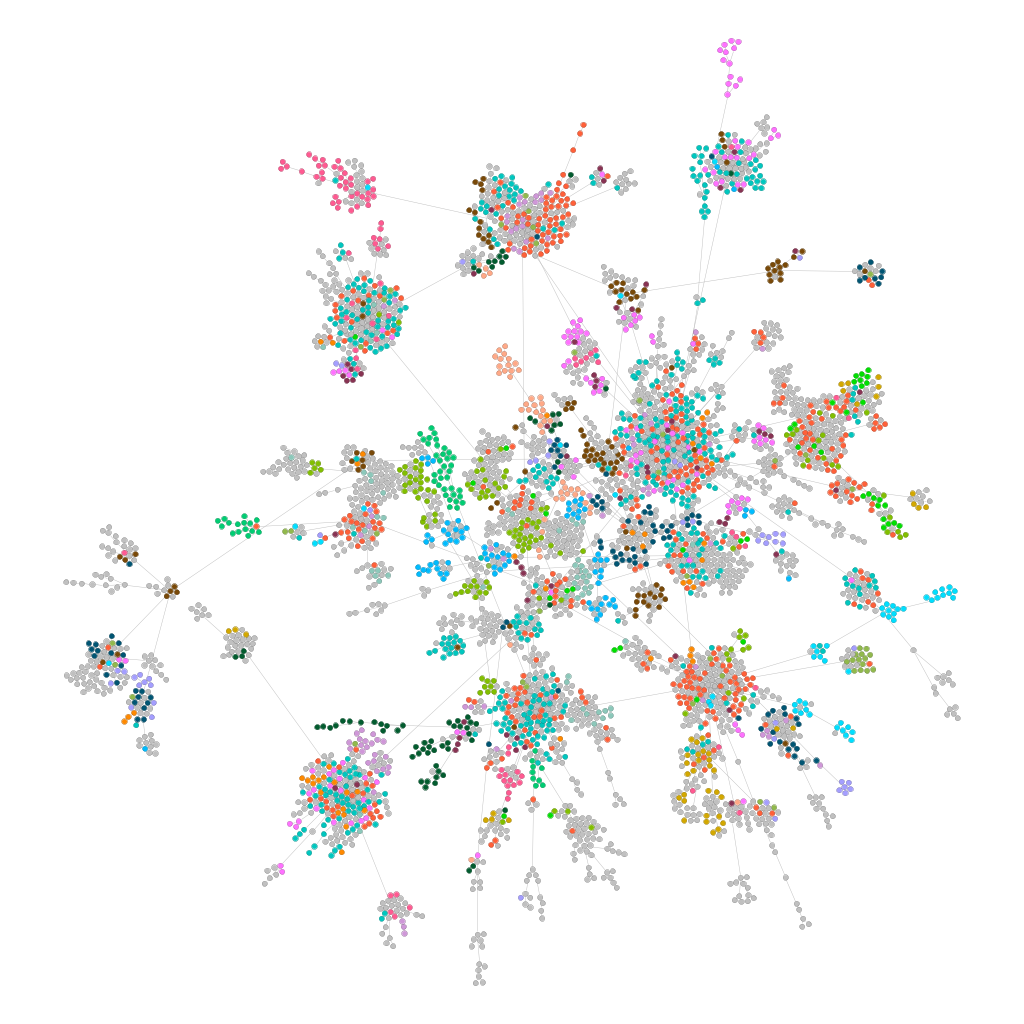
\includegraphics[width=\linewidth]{ari_test_0.1}
    \caption*{$\text{ARI}_{com}$ = 0.1}
    \end{subfigure}
    \hfill
    \begin{subfigure}[b]{0.495\textwidth}
            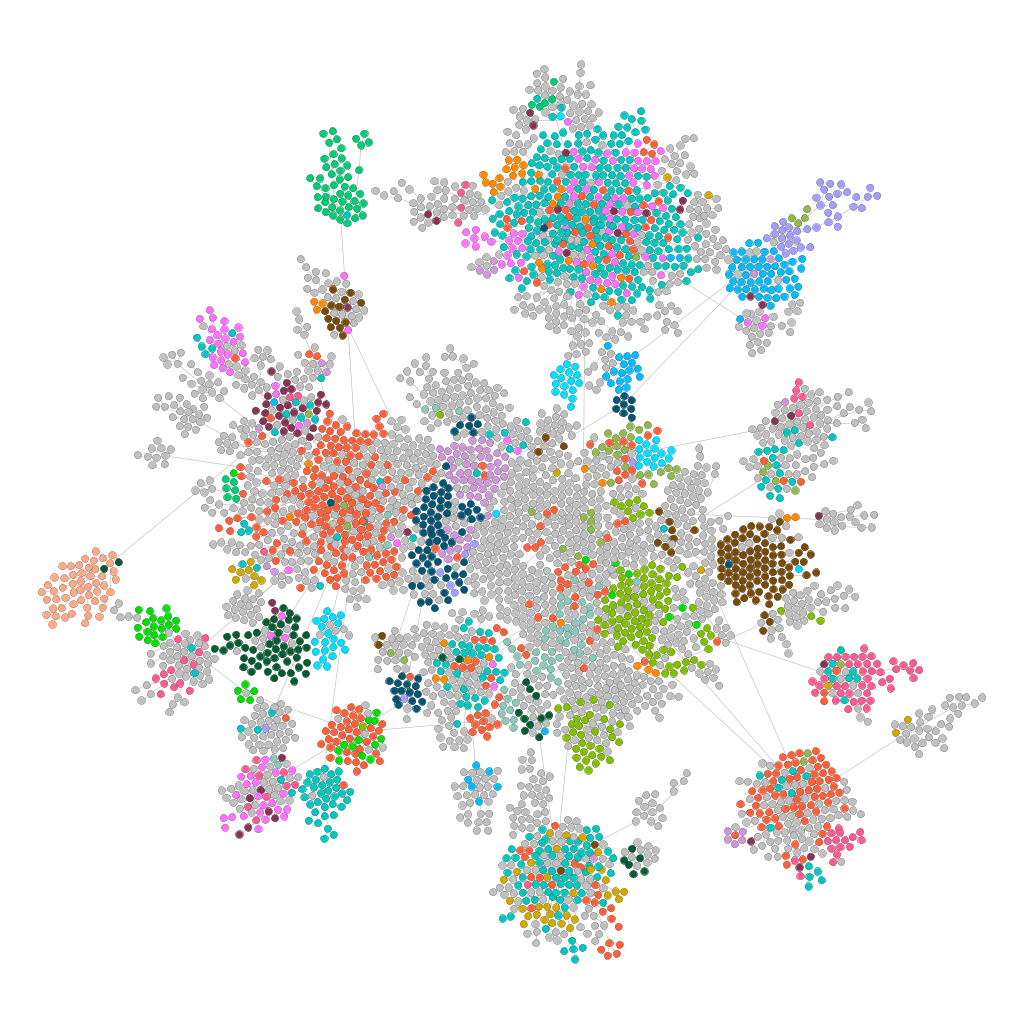
\includegraphics[width=\linewidth]{ari_test_0.3}
    \caption*{$\text{ARI}_{com}$ = 0.3}
    \end{subfigure}
  \hfill
    \begin{subfigure}[b]{0.495\textwidth}
            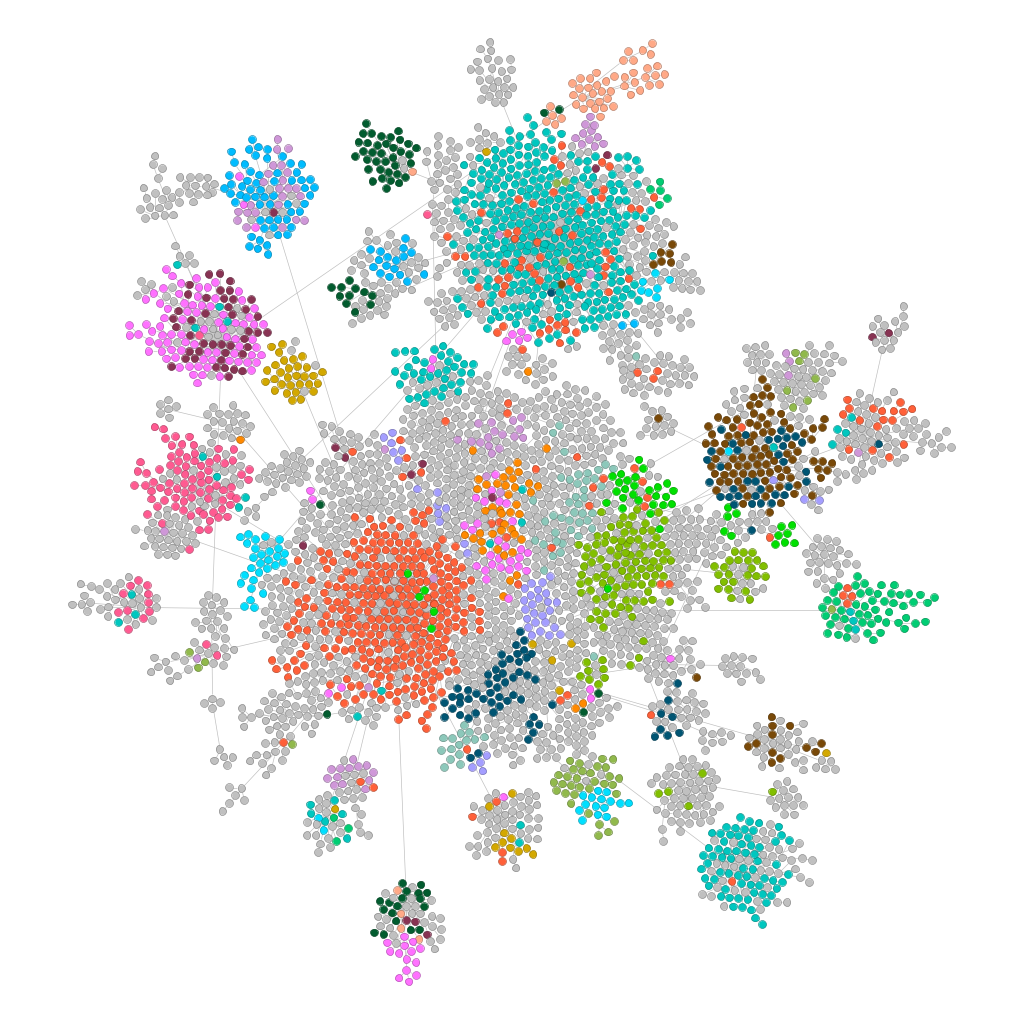
\includegraphics[width=\linewidth]{ari_test_0.5}
    \caption*{$\text{ARI}_{com}$ = 0.5}
    \end{subfigure}
  \hfill
    \begin{subfigure}[b]{0.495\textwidth}
            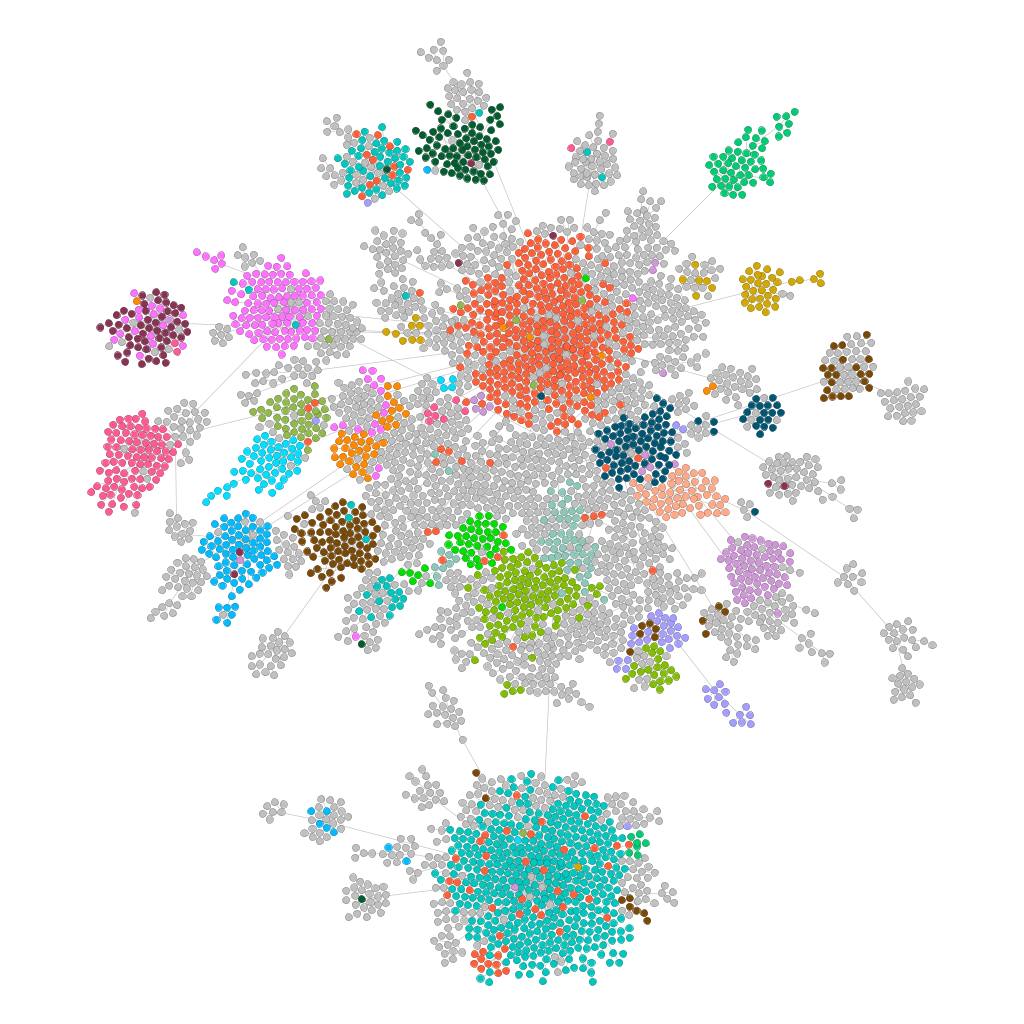
\includegraphics[width=\linewidth]{ari_test_0.7}
    \caption*{$\text{ARI}_{com}$ = 0.7}
    \end{subfigure}
    \caption{Impact of community \acrshort{ari} scores}
    \label{fig:community_ari_impact}
\end{figure}
\clearpage
  \begin{figure}[ht!]
  \centering
    \begin{subfigure}[b]{.8\textwidth}
            \includesvg[width=\linewidth]{optimized_dates_nrw_2022_10000}
    \caption*{(a) Sampling dates}
    \end{subfigure}
    \par\vspace{1em}
    \begin{subfigure}[b]{.8
    \textwidth}
            \includesvg[width=\linewidth]{optimized_cities_nrw_2022_10000}
    \caption*{(b) Cities of collection}
    \end{subfigure}
    \caption{Large-scale version of $T$\textsubscript{mod} for nrw\_2022 with 10,000 sequences}
    \label{fig:large_scale_sampling_date_optimized}
    \end{figure}
    \clearpage
  \begin{figure}[ht!]
  \centering
    \begin{subfigure}[b]{.8\textwidth}
            \includesvg[width=\linewidth]{lsh_nrw_2022_10000_dates}
    \caption*{(a) Sampling dates}
    \end{subfigure}
    \par\vspace{1em}
    \begin{subfigure}[b]{.8\textwidth}
            \includesvg[width=\linewidth]{lsh_nrw_2022_10000_cities}
    \caption*{(b) Cities of collection}
    \end{subfigure}
    \caption{Large-scale version of $T$\textsubscript{ACS} for nrw\_2022 with 10,000 sequences}
    \label{fig:large_scale_sampling_date_acs}
    \end{figure}
    \clearpage
\section{Supplementary Tables}
    \label{app:supplementary_tables}
    \begin{table}[ht!]
        \caption{Complete infection recall and community \acrshort{ari} scores for \acrshort{ccs}}
        \label{table:ccs_scores}
    \small
        \rotatebox{90}{%
            \begin{tabular}{c|c|c|c|c|c|c|c|c|c|c}
                \multirow{3}{*}{Search strategy}&\multicolumn{2}{c|}{Aggregate}& \multicolumn{8}{c}{Calculation rate}\\
                \cline{2-11}
                &\multirow{2}{*}{Size} & \multirow{2}{*}{Label} & \multicolumn{2}{c|}{0.05} & \multicolumn{2}{c|}{0.1} & \multicolumn{2}{c|}{0.15} & \multicolumn{2}{c}{0.2}\\
                \cline{4-11}
                &&&$\text{R}_{inf}$ & $\text{ARI}_{com}$ & $\text{R}_{inf}$ & $\text{ARI}_{com}$ & $\text{R}_{inf}$ & $\text{ARI}_{com}$ & $\text{R}_{inf}$ & $\text{ARI}_{com}$ \\
                \hline    
                \hline    
                Depth search&1,250& due\_202203 & 0.787 & 0.17 & 0.854 & 0.31 & 0.904 & 0.365 & 0.935 & 0.444 \\
                 \cline{3-11}
                && nrw\_202203 & 0.722 & 0.134 & 0.852 & 0.26 & 0.925 & 0.39 & 0.946 & 0.464 \\
                 \cline{3-11}
                && due\_2022 & 0.864 & 0.354 & 0.934 & 0.524 & 0.979 & 0.688 & 0.986 & 0.774 \\
                 \cline{3-11}
                && nrw\_2022 & 0.918 & 0.477 & 0.907 & 0.701 & 0.987 & 0.758 & 0.993 & 0.786 \\
                \cline{2-11}        
                & 2,500 & due\_202203 & 0.763 & 0.48 & 0.857 & 0.672 & 0.914 & 0.696 & 0.941 & 0.758 \\
                \cline{3-11}
                && nrw\_202203 & 0.764 & 0.212 & 0.867 & 0.323 & 0.915 & 0.429 & 0.947 & 0.511 \\
                \cline{3-11}
                && due\_2022 & 0.905 & 0.408 & 0.975 & 0.532 & 0.986 & 0.541 & 0.988 & 0.604 \\
                 \cline{3-11}
                && nrw\_2022 & 0.92 & 0.493 & 0.976 & 0.692 & 0.99 & 0.787 & 0.995 & 0.872 \\
                \cline{2-11}        
                &5,000 & due\_202203 & 0.767 & 0.275 & 0.826 & 0.263 & 0.869 & 0.333 & 0.909 & 0.336 \\
                 \cline{3-11}
                && nrw\_202203 & 0.803 & 0.268 & 0.91 & 0.406 & 0.945 & 0.544 & 0.967 & 0.624 \\
                 \cline{3-11}
                && due\_2022 & 0.914 & 0.378 & 0.971 & 0.537 & 0.985 & 0.619 & 0.99 & 0.675 \\
                 \cline{3-11}
                && nrw\_2022 & 0.942 & 0.423 & 0.979 & 0.601 & 0.993 & 0.77 & 0.995 & 0.853 \\
                \hline
                \hline    
                Breadth search&1,250 & due\_202203 & 0.364 & 0.175 & 0.55 & 0.217 & 0.666 & 0.266 & 0.747 & 0.257  \\
                 \cline{3-11}
                && nrw\_202203 & 0.406 & 0.115 & 0.594 & 0.212 & 0.714 & 0.209 & 0.785 & 0.277 \\
                 \cline{3-11}
                && due\_2022 & 0.659 & 0.318 & 0.801 & 0.43 & 0.873 & 0.43 & 0.911 & 0.528 \\
                 \cline{3-11}
                && nrw\_2022 & 0.768 & 0.472 & 0.894 & 0.549 & 0.929 & 0.617 & 0.937 & 0.769 \\
                \cline{2-11}        
                &2,500 & due\_202203 & 0.407 & 0.23 & 0.597 & 0.284 & 0.709 & 0.316 & 0.786 & 0.375 \\
                \cline{3-11}
                && nrw\_202203 & 0.422 & 0.139 & 0.606 & 0.226 & 0.713 & 0.283 & 0.776 & 0.379 \\
                \cline{3-11}
                && due\_2022 & 0.715 & 0.319 & 0.849 & 0.332 & 0.907 & 0.461 & 0.933 & 0.547 \\
                 \cline{3-11}
                && nrw\_2022 & 0.772 & 0.44 & 0.882 & 0.558 & 0.932 & 0.627 & 0.959 & 0.688  \\
                \cline{2-11}        
                &5,000 & due\_202203 & 0.431 & 0.177 & 0.591 & 0.228 & 0.704 & 0.263 & 0.786 & 0.294 \\
                 \cline{3-11}
                && nrw\_202203 & 0.469 & 0.131 & 0.657 & 0.188 & 0.756 & 0.265 & 0.822 & 0.396 \\
                 \cline{3-11}
                && due\_2022 & 0.706 & 0.308 & 0.843 & 0.389 & 0.907 & 0.441 & 0.933 & 0.472 \\
                 \cline{3-11}
                && nrw\_2022 & 0.809 & 0.389 & 0.915 & 0.492 & 0.956 & 0.591 & 0.972 & 0.654 \\
            \end{tabular}  
            }    
        \end{table}
        \clearpage
\setcounter{table}{0}
\section{Code base}
The code base to this work is available in a public GitHub repository at \url{https://github.com/benjoka/thesis_bk}. Table \ref{table:code_base_structure} describes the directory structure of the code base.

\renewcommand{\arraystretch}{1.5}
\begin{table}[H]
\centering
\caption{Directory structure of the code base}
\label{table:code_base_structure}
\begin{tabular}{>{\centering\arraybackslash}p{0.2\textwidth}|>{\centering\arraybackslash}p{0.7\textwidth}}
Directory & Description \\
\hline\hline
results & Results of the thesis. Scores of \acrshort{acs} might differ from the concrete scores listed in the thesis, as the procedure does not produce unambiguous results. The order of directories reflects the order results are presented in the thesis. \\
\hline
gendisc & Golang package that implements the GENTRAIN algorithm to calculate genetic distances. When executed with \texttt{--fast} the adjustments proposed in this work are used. \\
\hline
gentrain & Python module with the implementations of the approaches proposed in the thesis and several helper functions for evaluation purposes. \\
\hline
latex & LaTeX files of the thesis. \\
\end{tabular}
\end{table}
\clearpage
\setcounter{table}{0}
\section{Software and Hardware Used}
 \begin{table}[ht!]
    \caption{Software used}
    \label{table:software}
        \begin{threeparttable}
            \begin{tabular}{Sc|Sc|Sc}
                Software & Version & Purpose \\
                \hline\hline
                GoLand & 2024.3.4 & Golang programming \\
                \hline
                PyCharm & 2024.2.5 & Python Programming, Jupyter Notebooks \\
                \hline
                scikit-learn & 1.6.1 & Data analysis \\
                \hline
                pandas & 2.2.3 & Data analysis and manipulation \\
                \hline
                NumPy & 2.0.0 & Data analysis and manipulation \\
                \hline
                jupyter & 1.1.1 & Results preparation and presentation \\
                \hline
                HNSWlib & 0.8.0 & \acrshort{acs} benchmarking \\
                \hline
                Biopython & 1.85 & Fasta file processing \\
                \hline
                NetworkX & 3.4.2 & Graph creation and manipulation \\
                \hline
                Plotly & 6.2.0 & Plot creation \\
                \hline
                Gephi & 0.10.1 & Graph visualization and configuration \\
                \hline
                Adobe Illustrator & 29.5 & SVG processing \\
                \hline
                Canva & - & Aggregate figure creation \\
                \hline
                Deepl Write\textsuperscript{a} & - & AI-driven grammar and spelling correction \\
                \hline
                Writefull\textsuperscript{a} & - & AI-driven grammar and spelling correction \\
                \hline
                Google Scholar & - & Literature research \\
                \hline
                Consensus\textsuperscript{a} & - & AI-driven literature research \\
            \end{tabular}
            \begin{tablenotes}[flushleft]
                \small
                \item[a] AI tools were used with careful supervision and all scientific contributions are solely my own.
            \end{tablenotes}
        \end{threeparttable}
\end{table}
 \begin{table}[ht!]
    \caption{Hardware used}
    \label{table:hardware}
    \resizebox{\textwidth}{!}{%
        \begin{tabular}{Sc|Sc|Sc|Sc}
        Model & Processor (CPU) & Memory (RAM) & Operating System \\
        \hline\hline
        MacBook Air (2020) & Apple M1, 8-core CPU & 16 GB & macOS Sonoma 14.2.1\\
        \end{tabular}
    }
\end{table}
    
    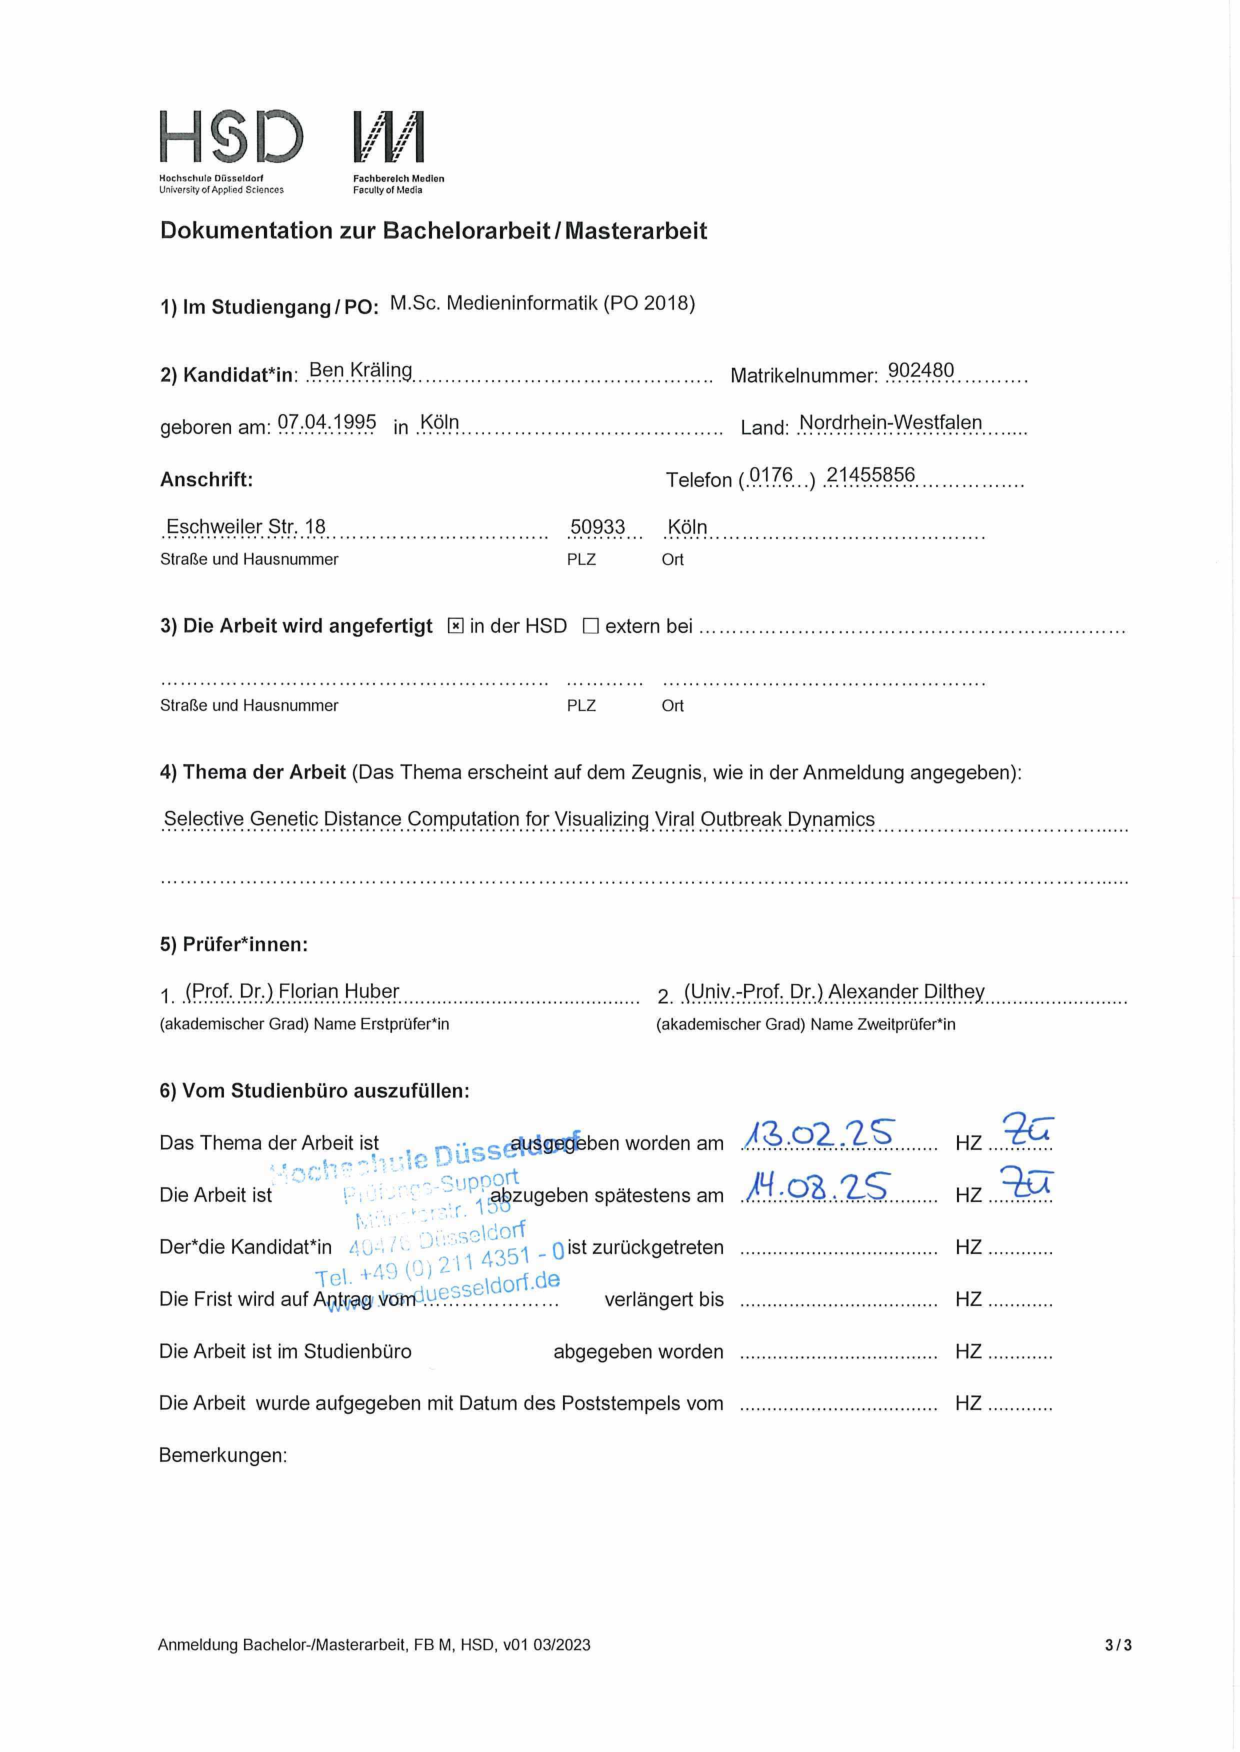
\includepdf[pages=-]{pages/laufzettel.pdf}
\end{document}

